\chapter{Results}

In this section, we will present our calculations performed for the 2D Hubbard model based on DMFT and Dual Fermion calculations. We will discuss some results of densities, Green's functions, self- energy, susceptibility, correlation length and transition from Fermi liquid state to non-Fermi liquid state. 
As we mentioned before, to solve a strongly correlated system one of the best methods is the Dynamical Mean Field Theory. In this method, we use the continuous-time auxiliary-field algorithm (CT-AUX) as an impurity solver. The results of DMFT are the input to Dual fermion approach.



\section{Density of states}

In Fig. \ref{fig:density_beta} we represent the density, $n$, versus chemical potential, $\mu$ , the slope of which is the compressibility $\kappa= \frac{\partial n}{\partial \mu}$. These plots found by DMFT methods, for different interaction strengths $(U=3, 5, 8)$. The left plot is for $\beta=2$ and the right plot is for $\beta=5$, also the next-nearest neighbour hopping parameter is $(t'=0)$. In these curves the density is:
\begin{equation}
    n=<n_{\uparrow}+\: n_{\downarrow}>
\end{equation}

Where $(\uparrow, \downarrow)$ describe the spin. It can be seen that by increasing $\beta$ (decreasing temperature), the slope of curves increases. On the other hand, by decreasing $\beta$ the slop of curves near half filling point  
increases, which this slope decreasing in the density vs $\mu$  show its effect in the spectral function, where a gap start to appears and represents a transition between metal and insulator, and the reason for this transition is that there is no state that electron can exist in that states so the system would be an insulator. Moreover, increasing the interaction strengths around half-filling has the same result. These results are depicted in Fig. \ref{fig:DMFT_spectral}
 
 \begin{figure}[ht]
\centering
    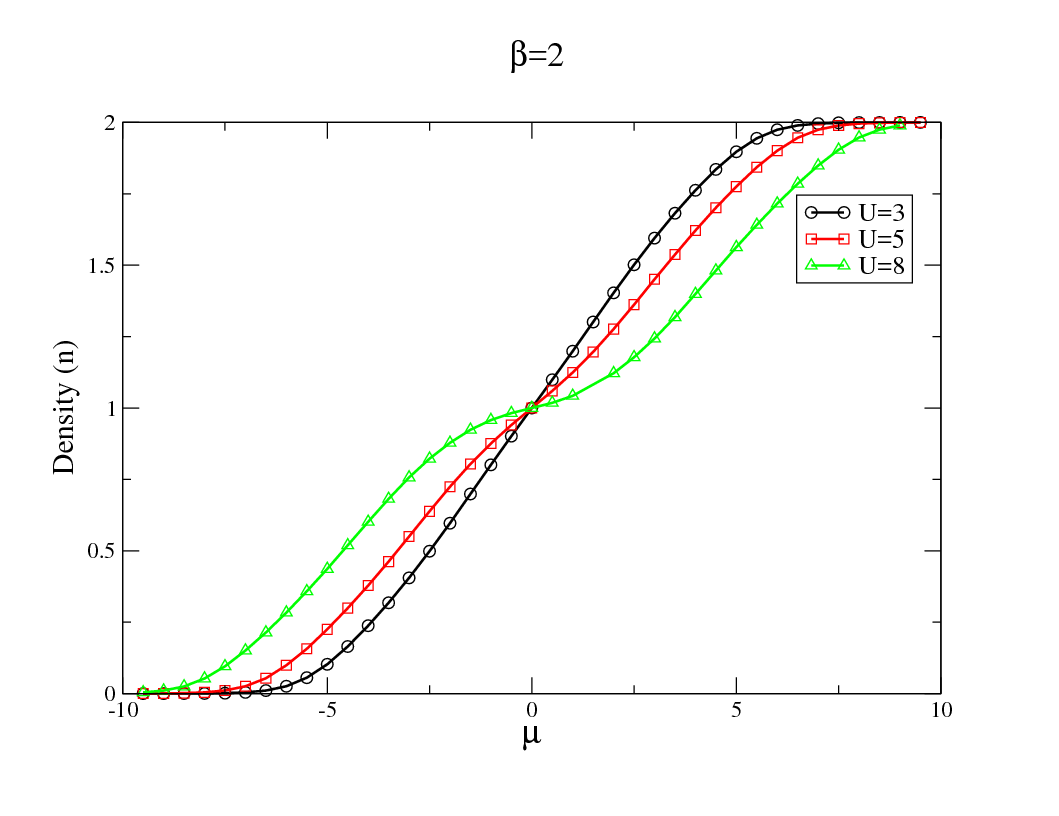
\includegraphics[width=0.47\linewidth]{fig3/density_betat.png}
    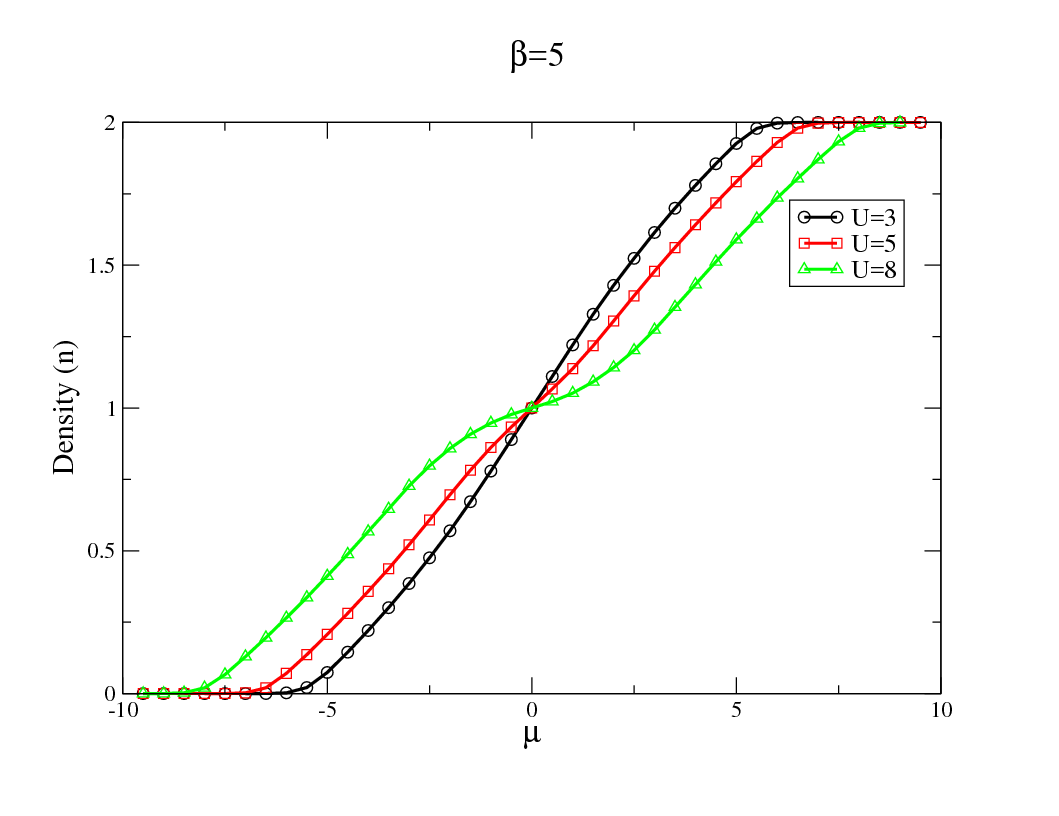
\includegraphics[width=0.47\linewidth]{fig3/density_betaf.png}
    
\caption{Density vs $\mu$ based on single site DMFT results for different interaction strength $U=3, 5, 8$. In the left plot $\beta = 2$ and the right plot $\beta = 5$ and $t'=0$.
\label{fig:density_beta}}
\end{figure}
 
 
 Density in the DMFT method is obtained from $G(i \omega _n)$ which does not depend on momentum, but we have employed Dual Fermion method and this provides $G(i \omega _n ,k)$. We now have access to momentum space by this correction and we can again find density vs chemical potential. In Fig. \ref{fig:df_density} it can be seen that around the half-filling the curve is flat for $U=5.6$ and $U=8$. In this plot we used $\beta = 5$ and $t'=-0.3$.This flattening shows a reduction in the compressibility of the system $(\kappa= \frac{\partial n}{\partial \mu})$, and this reduction represents an electronic gap, which means there would be a transition from metallic to insulating states.

 
 \begin{figure}[ht]
\centering
    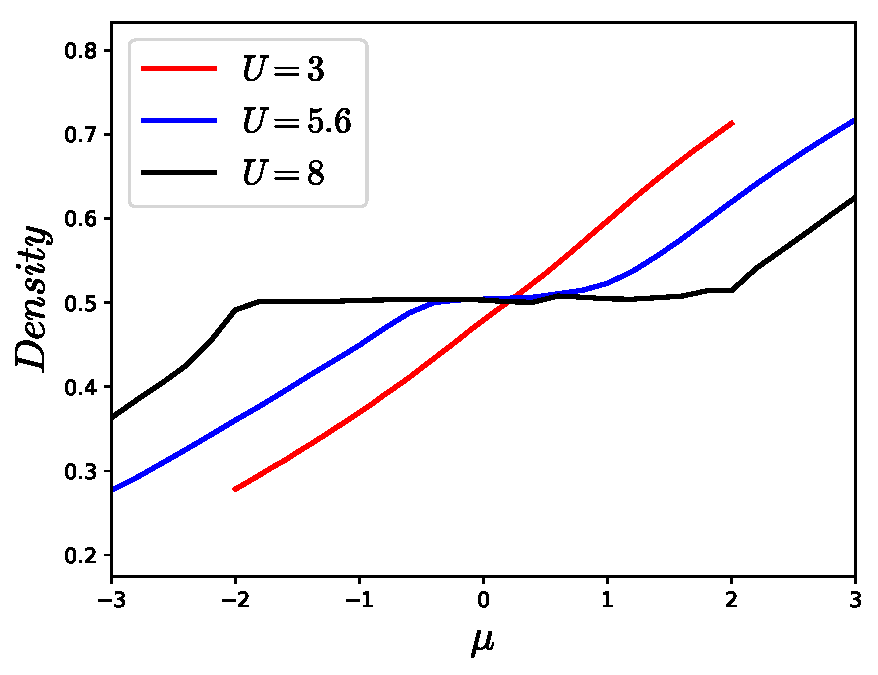
\includegraphics[width=0.6\linewidth]{fig3/df_density_mu.pdf}
    
\caption{Density vs $\mu$ based on Dual Fermion approach for different interaction strength $(U=3, 5.6, 8)$ and  $\beta = 5$ and $t'=-0.3$.
\label{fig:df_density}}
\end{figure}
 
\noindent The corrections from Dual Fermions become important at bigger interaction strengths around half-filling, and make the curve of  $n$ versus $\mu$ flat. The hopping $t'$ brakes particle-hole symmetry, so that the curve is not symmetric around half-filling, $\mu$. DF shows Insulator behaviour for lower $U$ values that from DMFT. 


The spectral function's plots are obtained by analytically continuing the Green's functions found by DMFT and dual fermions, via the Maximum Entropy method \cite{M.Jarrell} which we discussed before. In chapter 2 we showed the relation between the spectral function and Green's function which is:

\begin{equation}
    A(\omega) = -\frac{1}{\pi}Im[G(\omega)].
\end{equation}

The result of DMFT is a local Green's function which is a function of frequency, but Dual Fermion calculations produce a Green's function which has momentum as well, $G(i\omega _n , k)$, therefore to find local Dual Green's function we have to integrate over $k$. The density of state or local $(r=0)$ spectral function for Dual Fermion can be written as:

\begin{equation}
    A^{DF} (\omega) = -\frac{1}{\pi} Im[\frac{1}{N_k}\sum _k G^{DF} (i\omega _n , k)],
\end{equation}

\noindent where $N_k$ is the number of momentum points.
In the Fig. \ref{fig:DMFT_spectral} the spectral function obtained from DMFT is symmetric. In the small interaction $(U=5)$ where it's called weakly correlated regime, electrons can be described as quasiparticles which their density of state still resembles free electrons. In strongly correlated regime $U= 8, 9$, the spectral function displays a three-peak structure. When the interaction between electrons are strong, $U=12$ the metal-insulator transition occurs and force the quasiparticle peak to vanish. 

In Fig. \ref{fig:DF_spectral} the spectral function of Dual Fermions has been shown. As we used $t'=-0.3$, it breaks the particle-hole symmetry of our the system, the asymmetry of the spectral functions with frequency can be seen here. Moreover, to make a comparison between Fig. \ref{fig:DMFT_spectral} and Fig. \ref{fig:DF_spectral} it can be seen that the gap of Dual Fermion at smaller U $(U=8)$ starts to open, while in DMFT the gap opens for bigger U $(U=11)$. 

Dual Fermion method can produce data with any momentum space resolution that we need at lower expenses. So, Dual fermions let us to study the behaviour of Green's functions and spectral functions in the Brillouin zone. This can be advantageous for momentum dependent systems, and to make a comparison between data of simulations and data which directly come from the experimental techniques, such as ARPES \cite{Zahid}.


\begin{figure}[ht]
\centering
    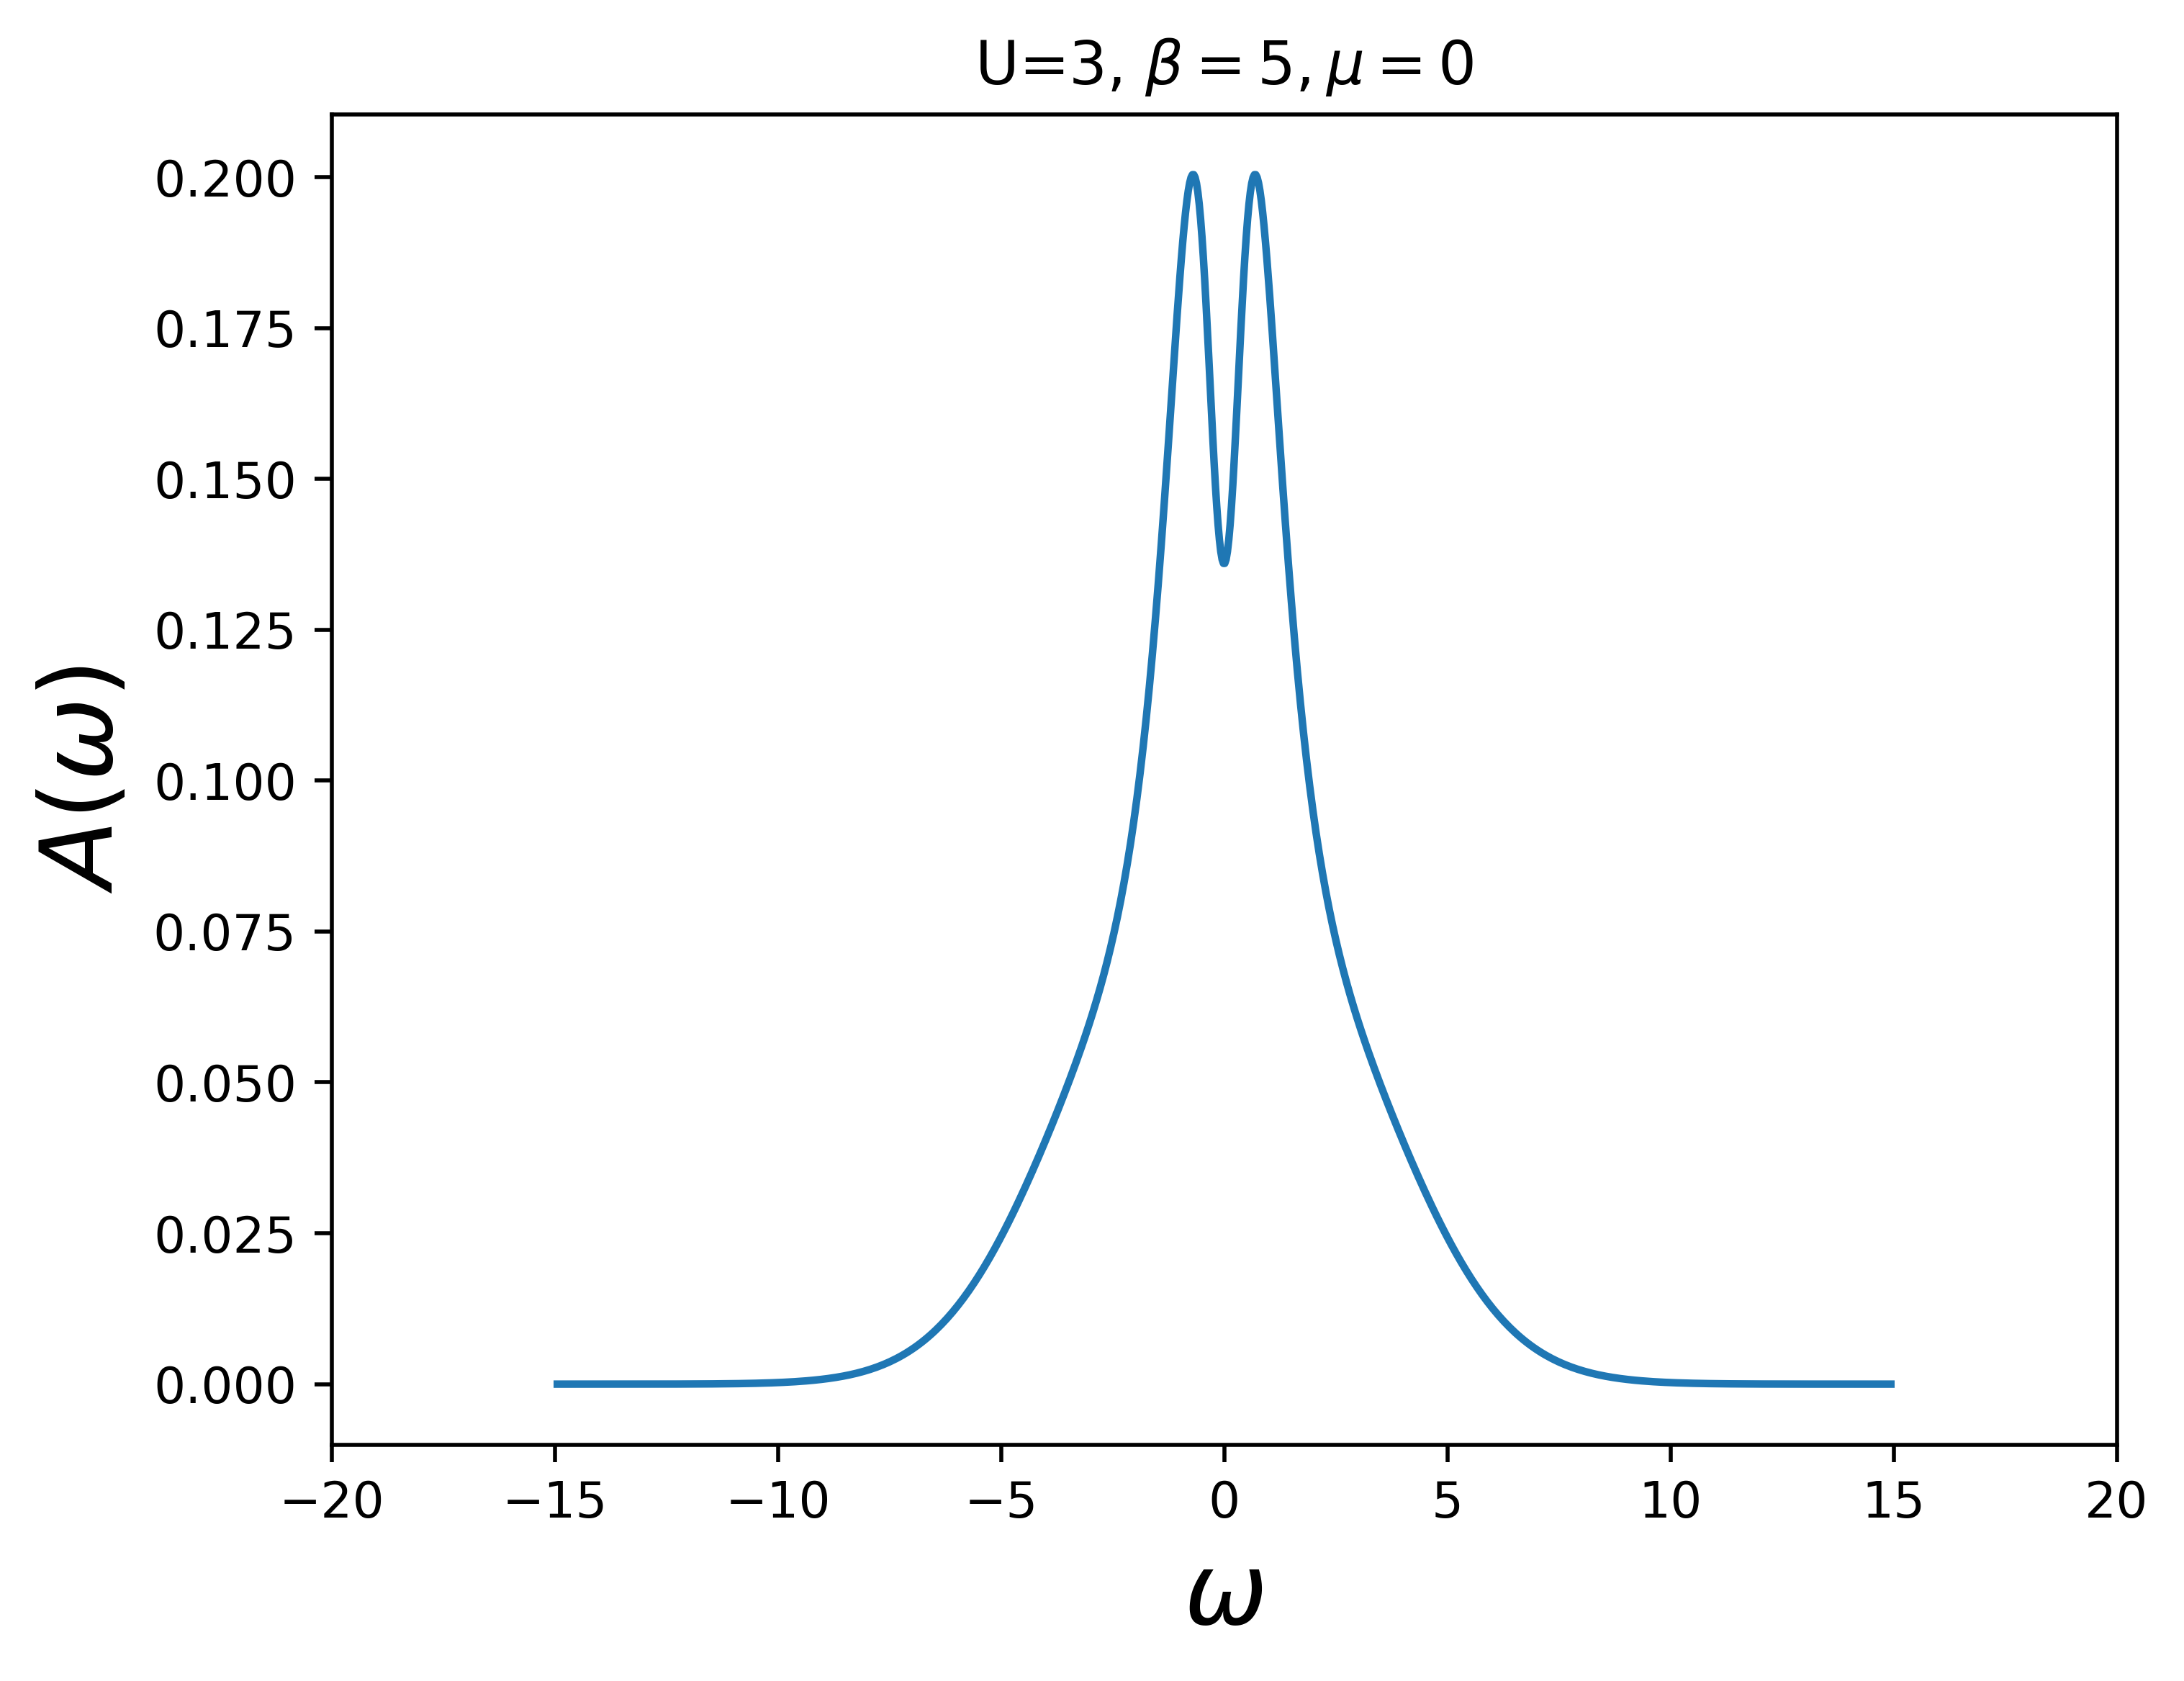
\includegraphics[width=0.45\linewidth]{fig2/spectral3.png}
     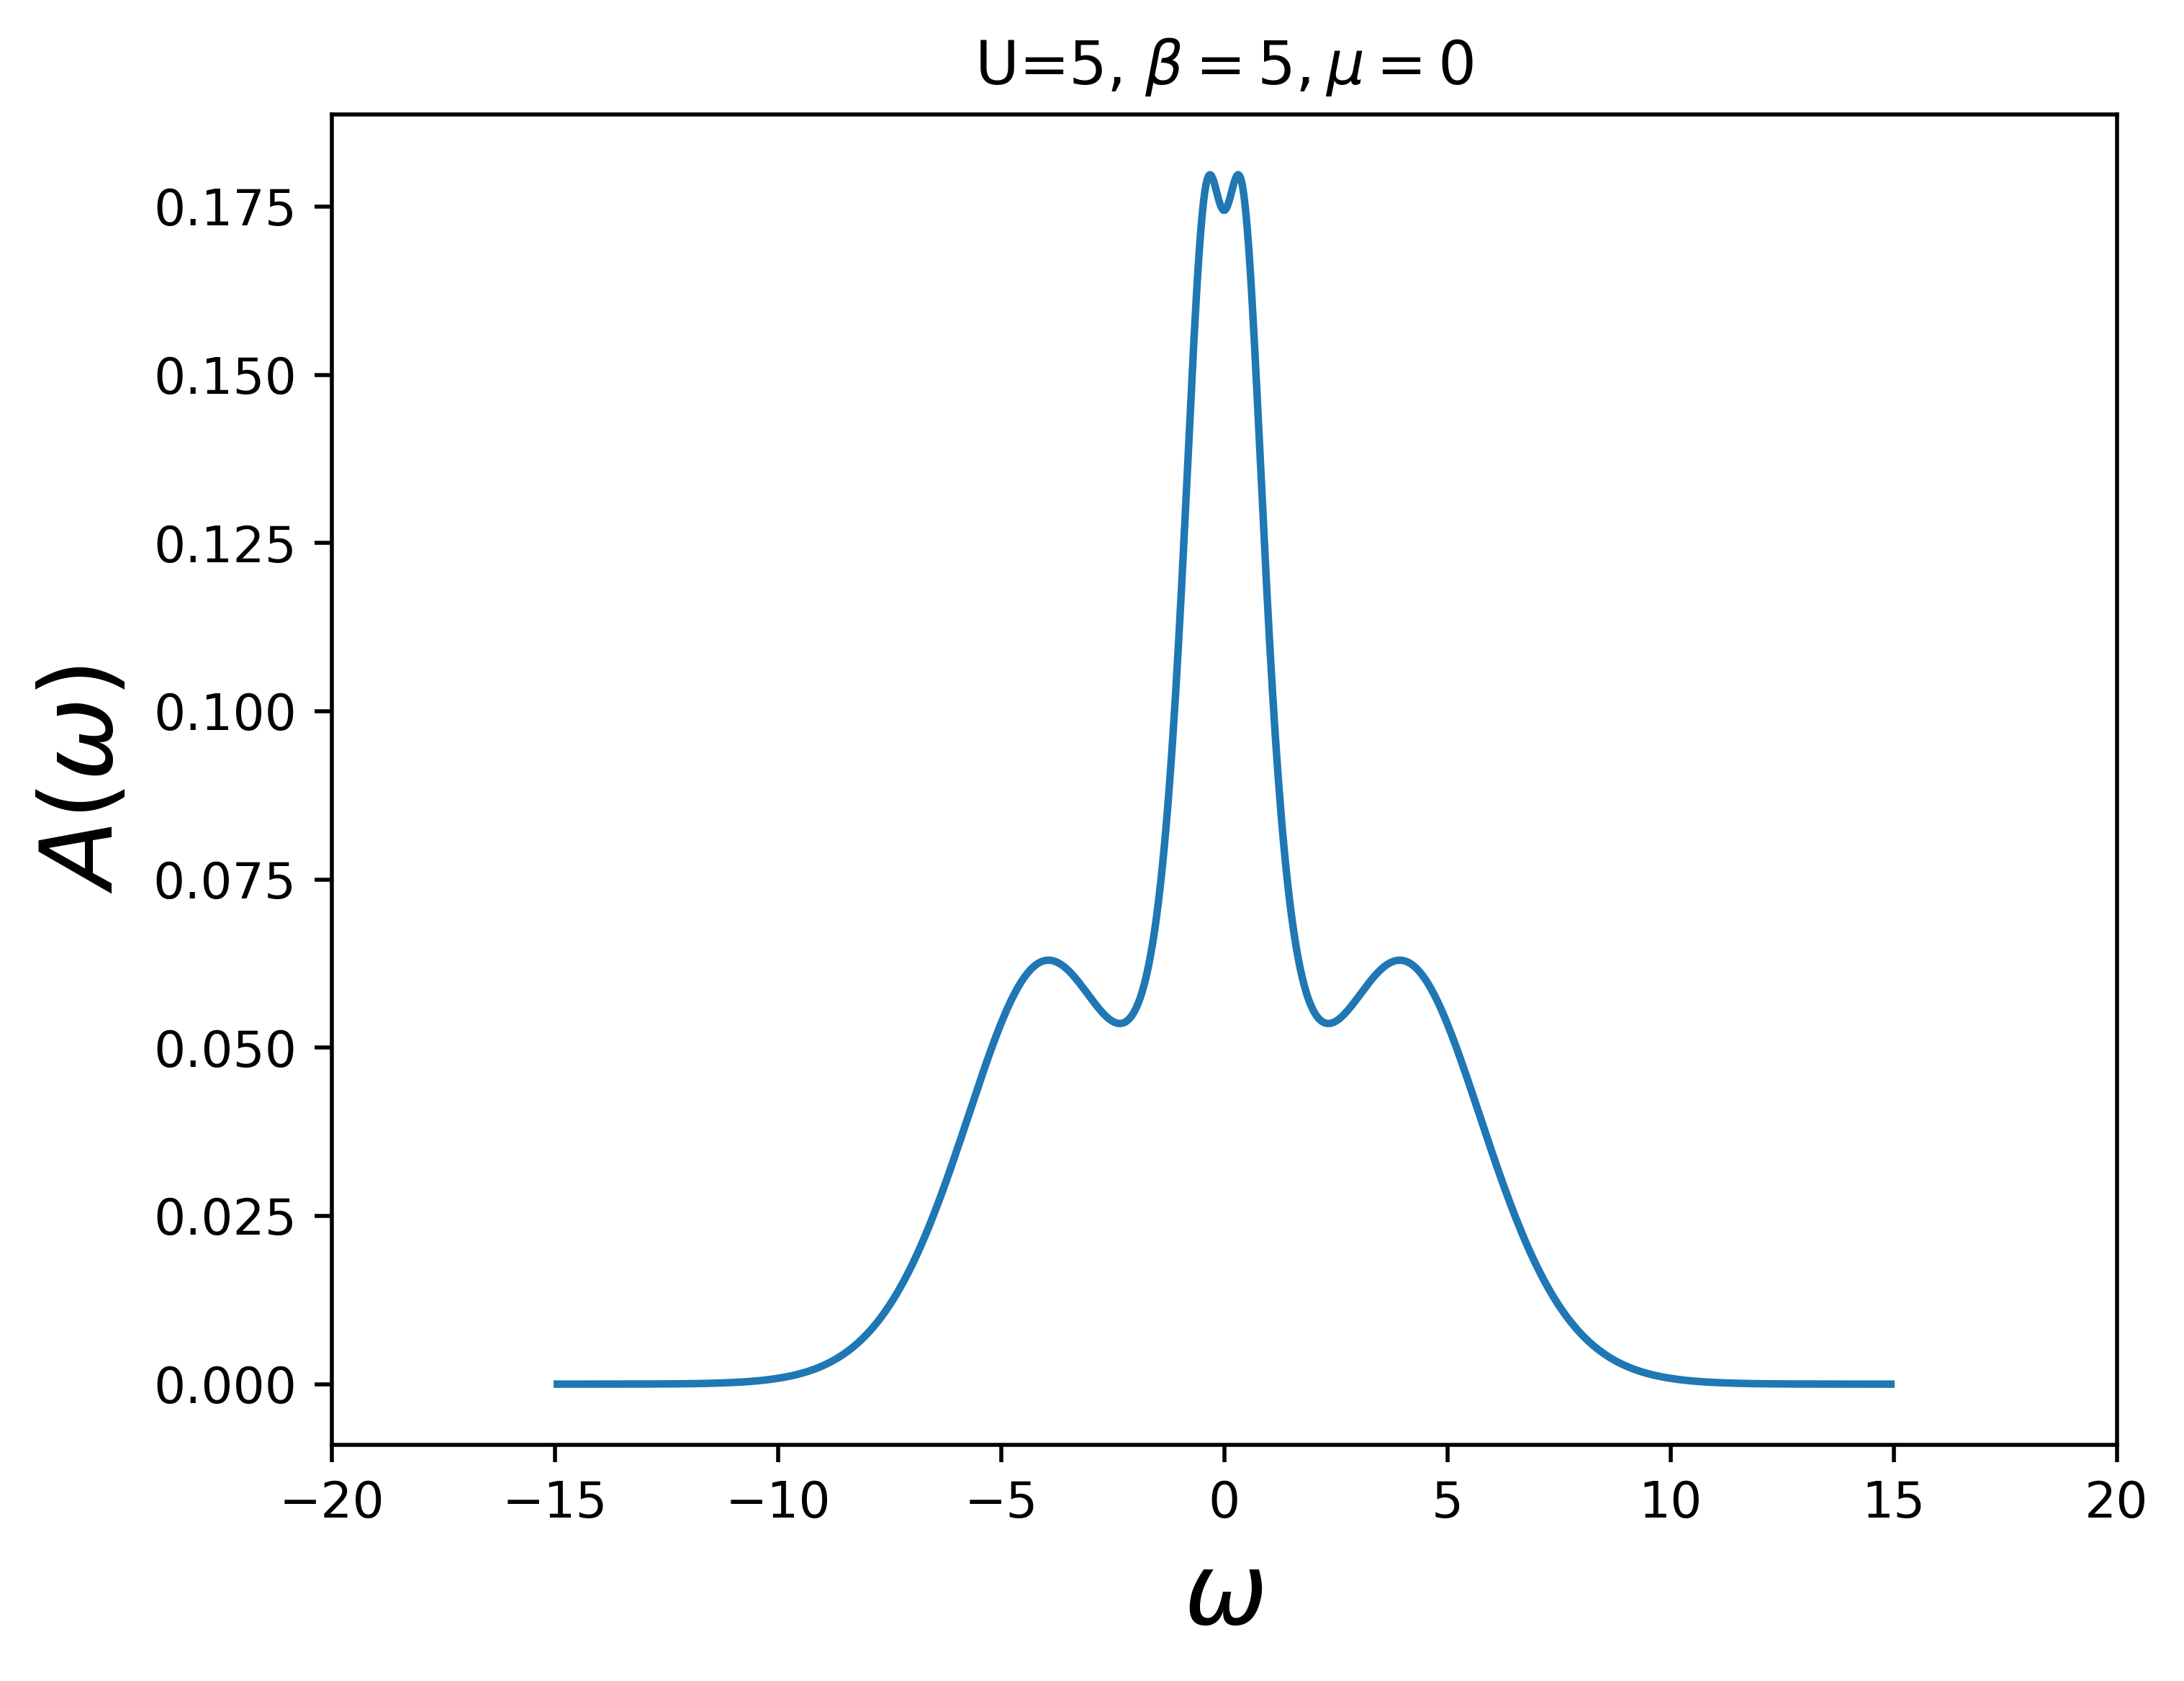
\includegraphics[width=0.45\linewidth]{fig2/spectral5.png}
      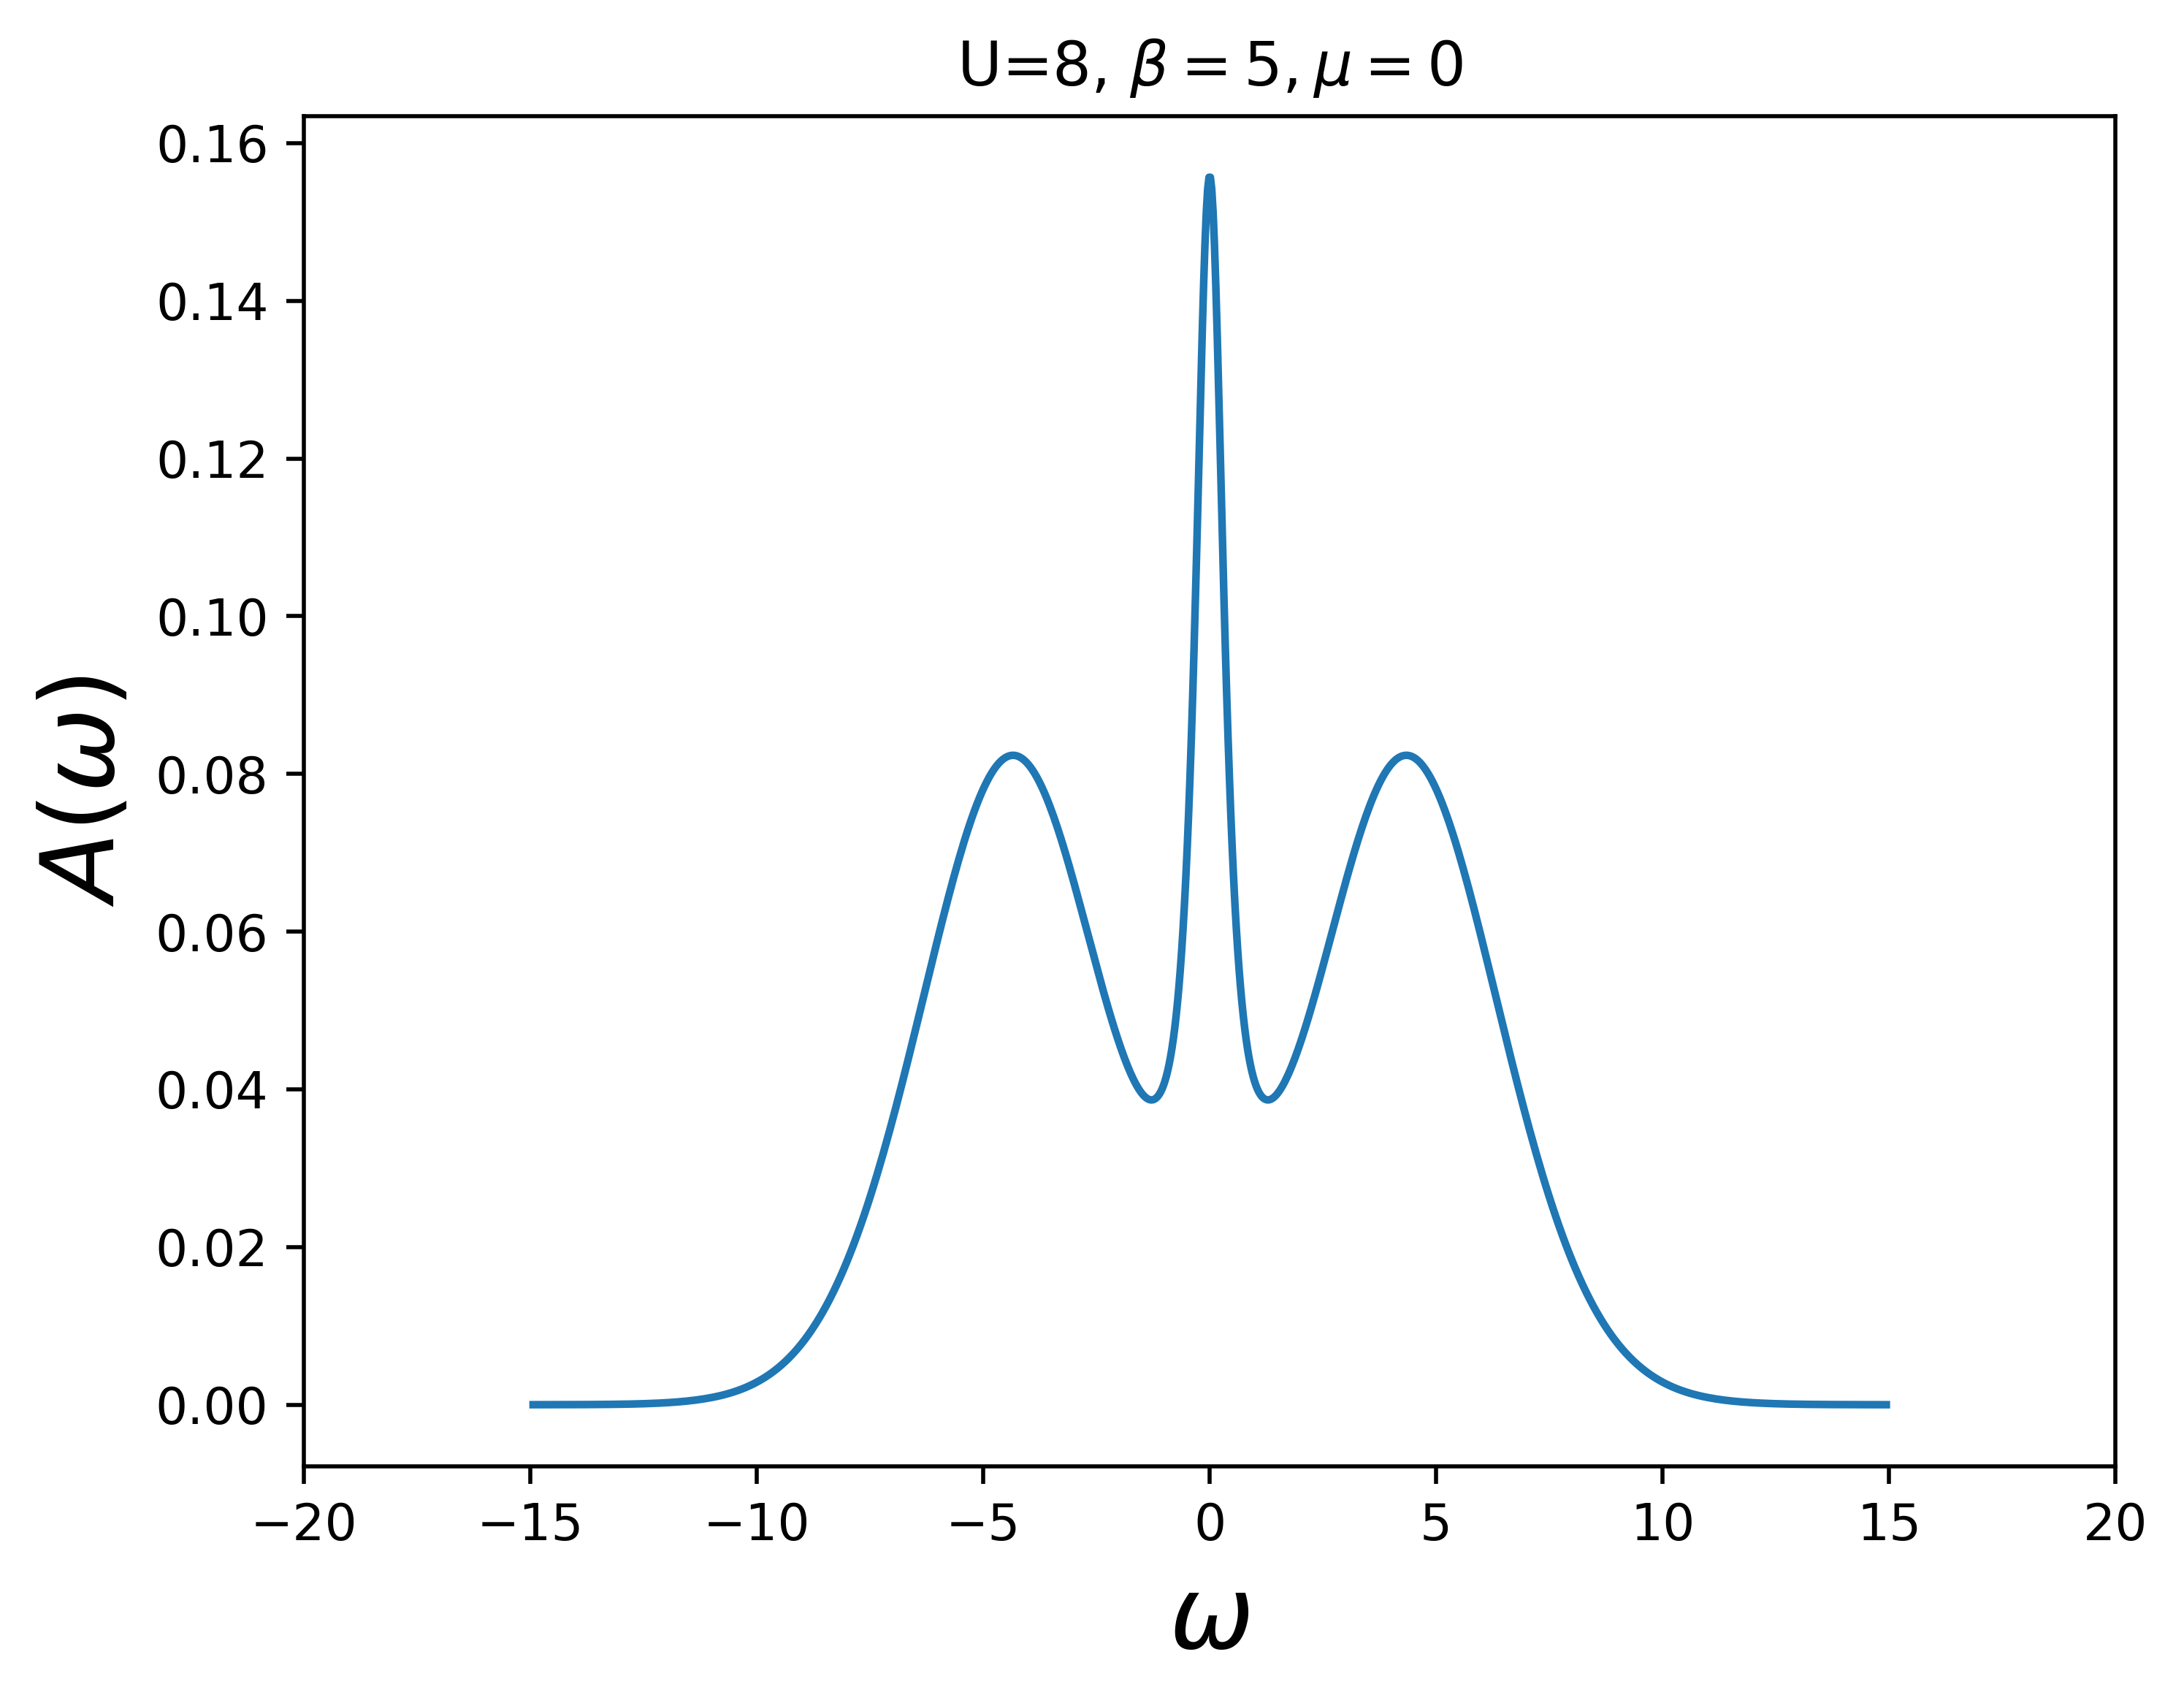
\includegraphics[width=0.45\linewidth]{fig2/spectral8.png}
       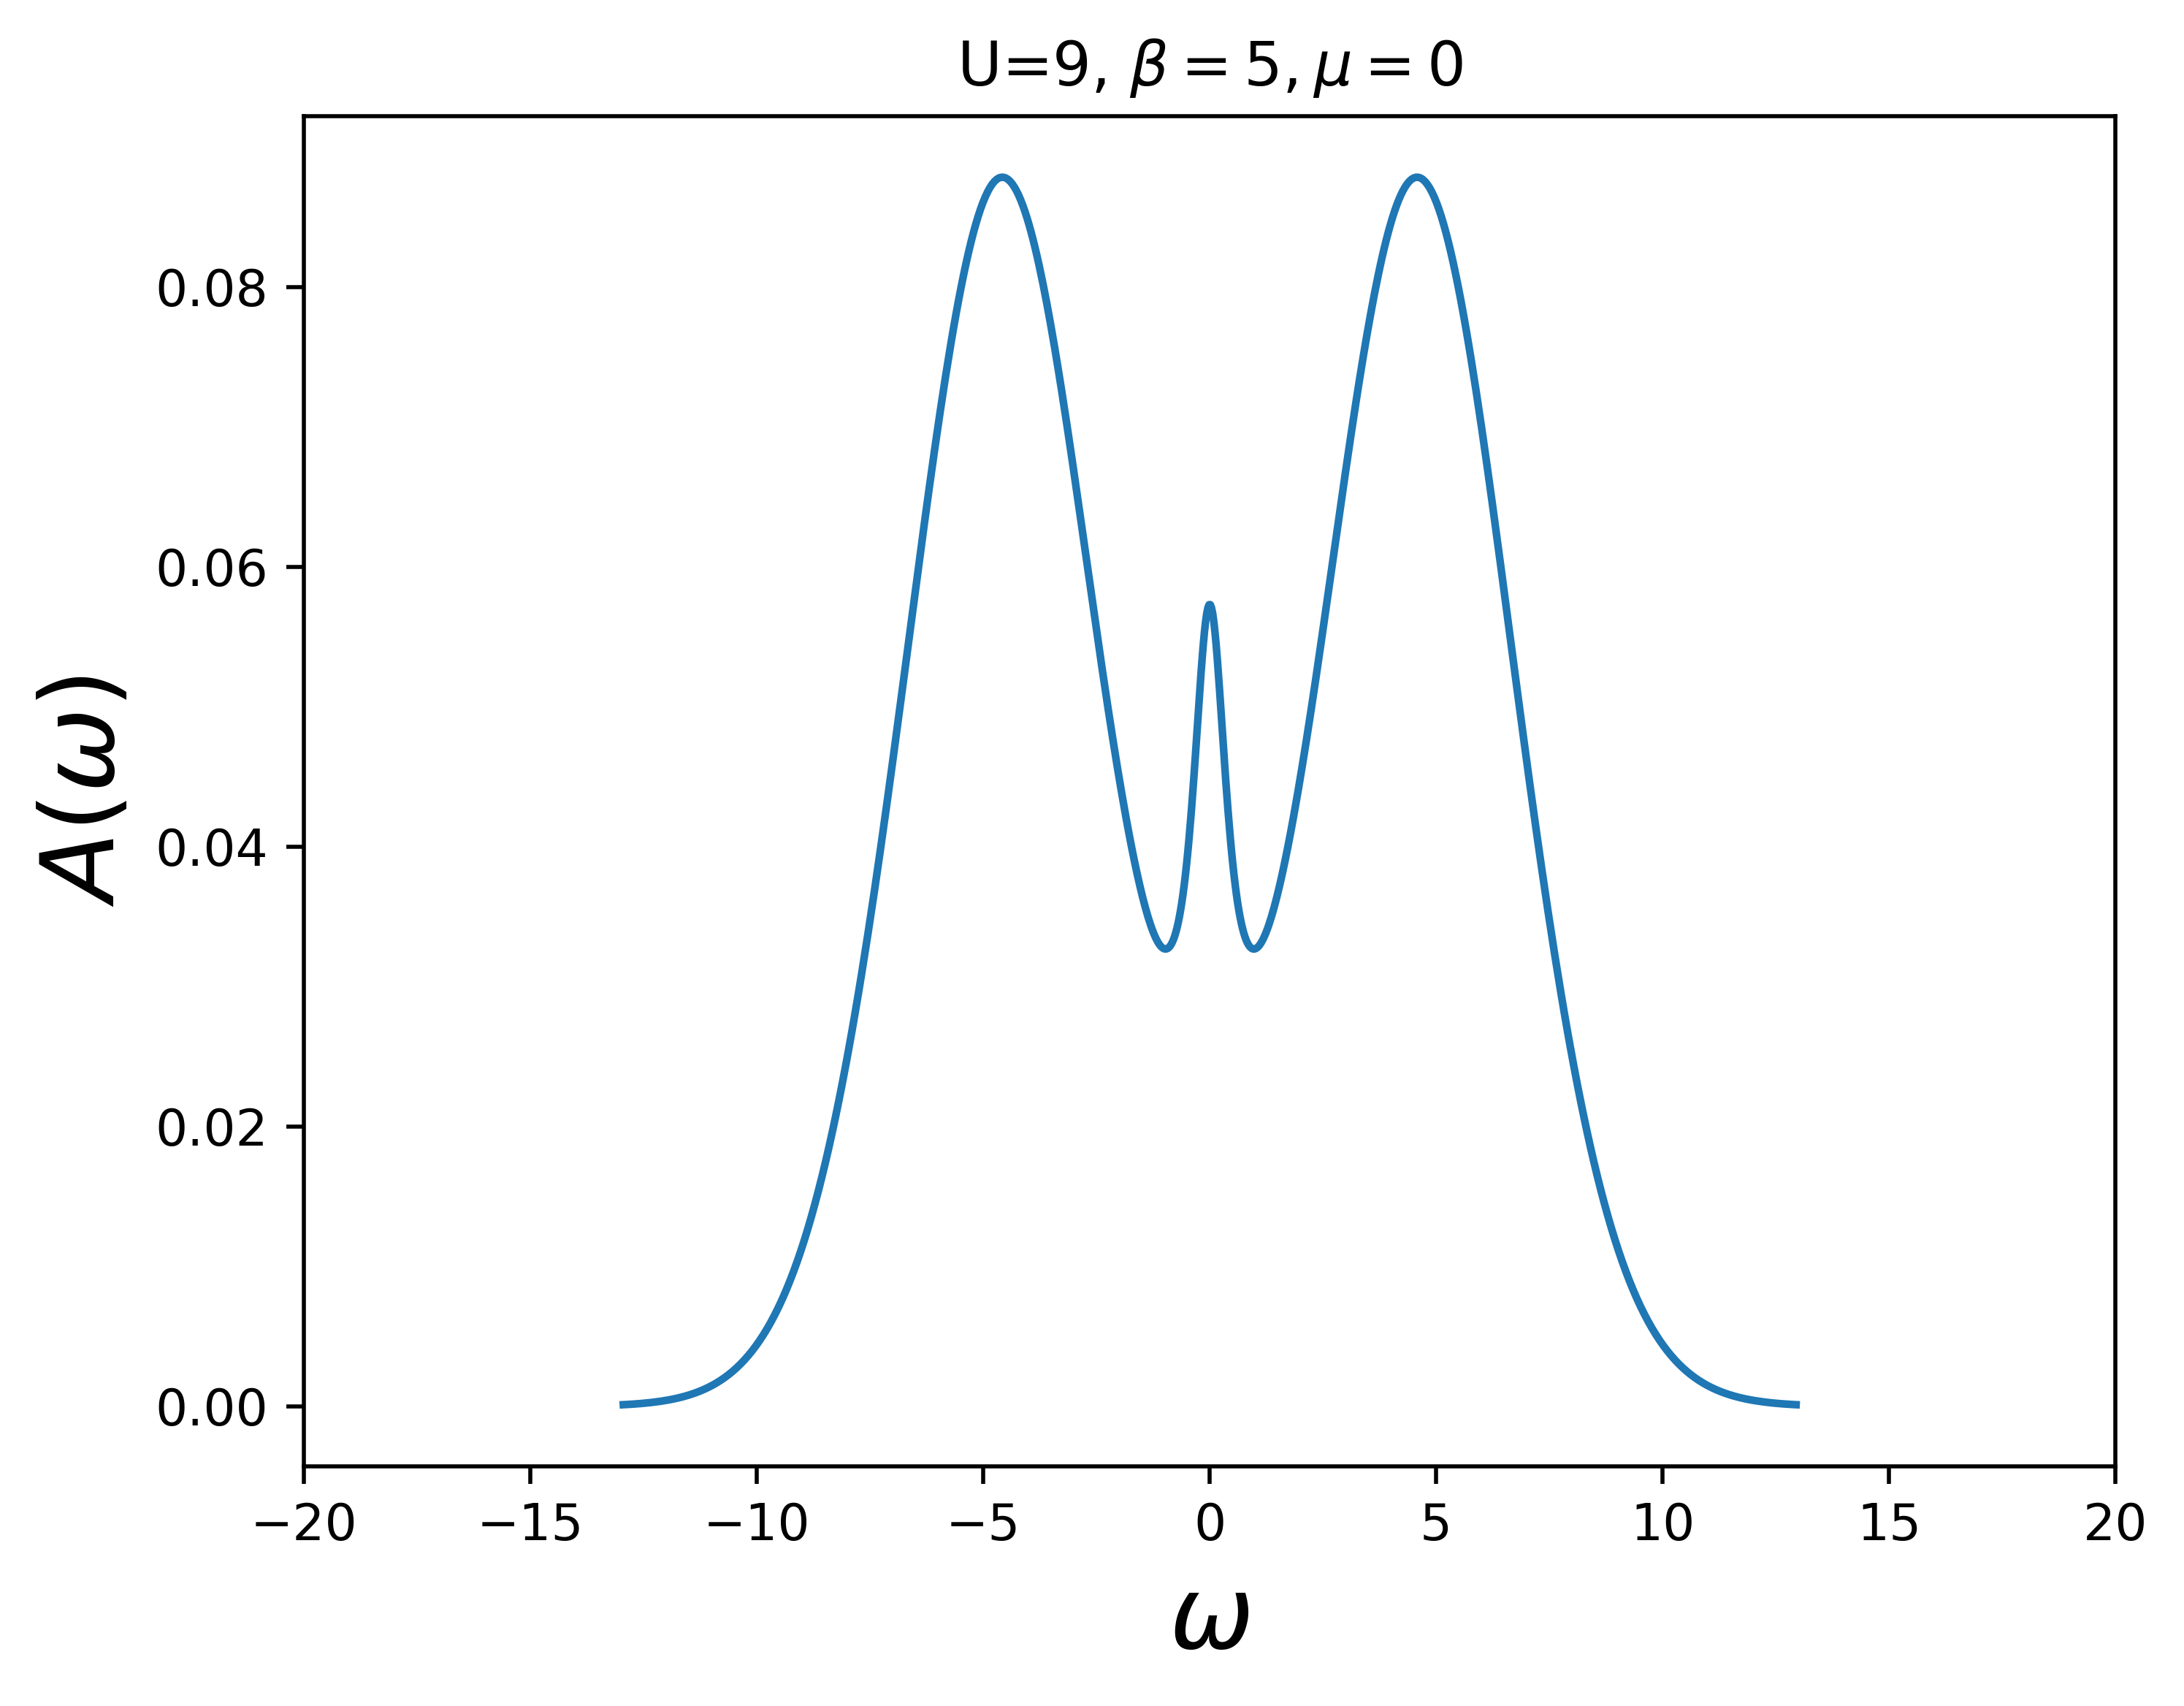
\includegraphics[width=0.45\linewidth]{fig2/spectral9.png}
        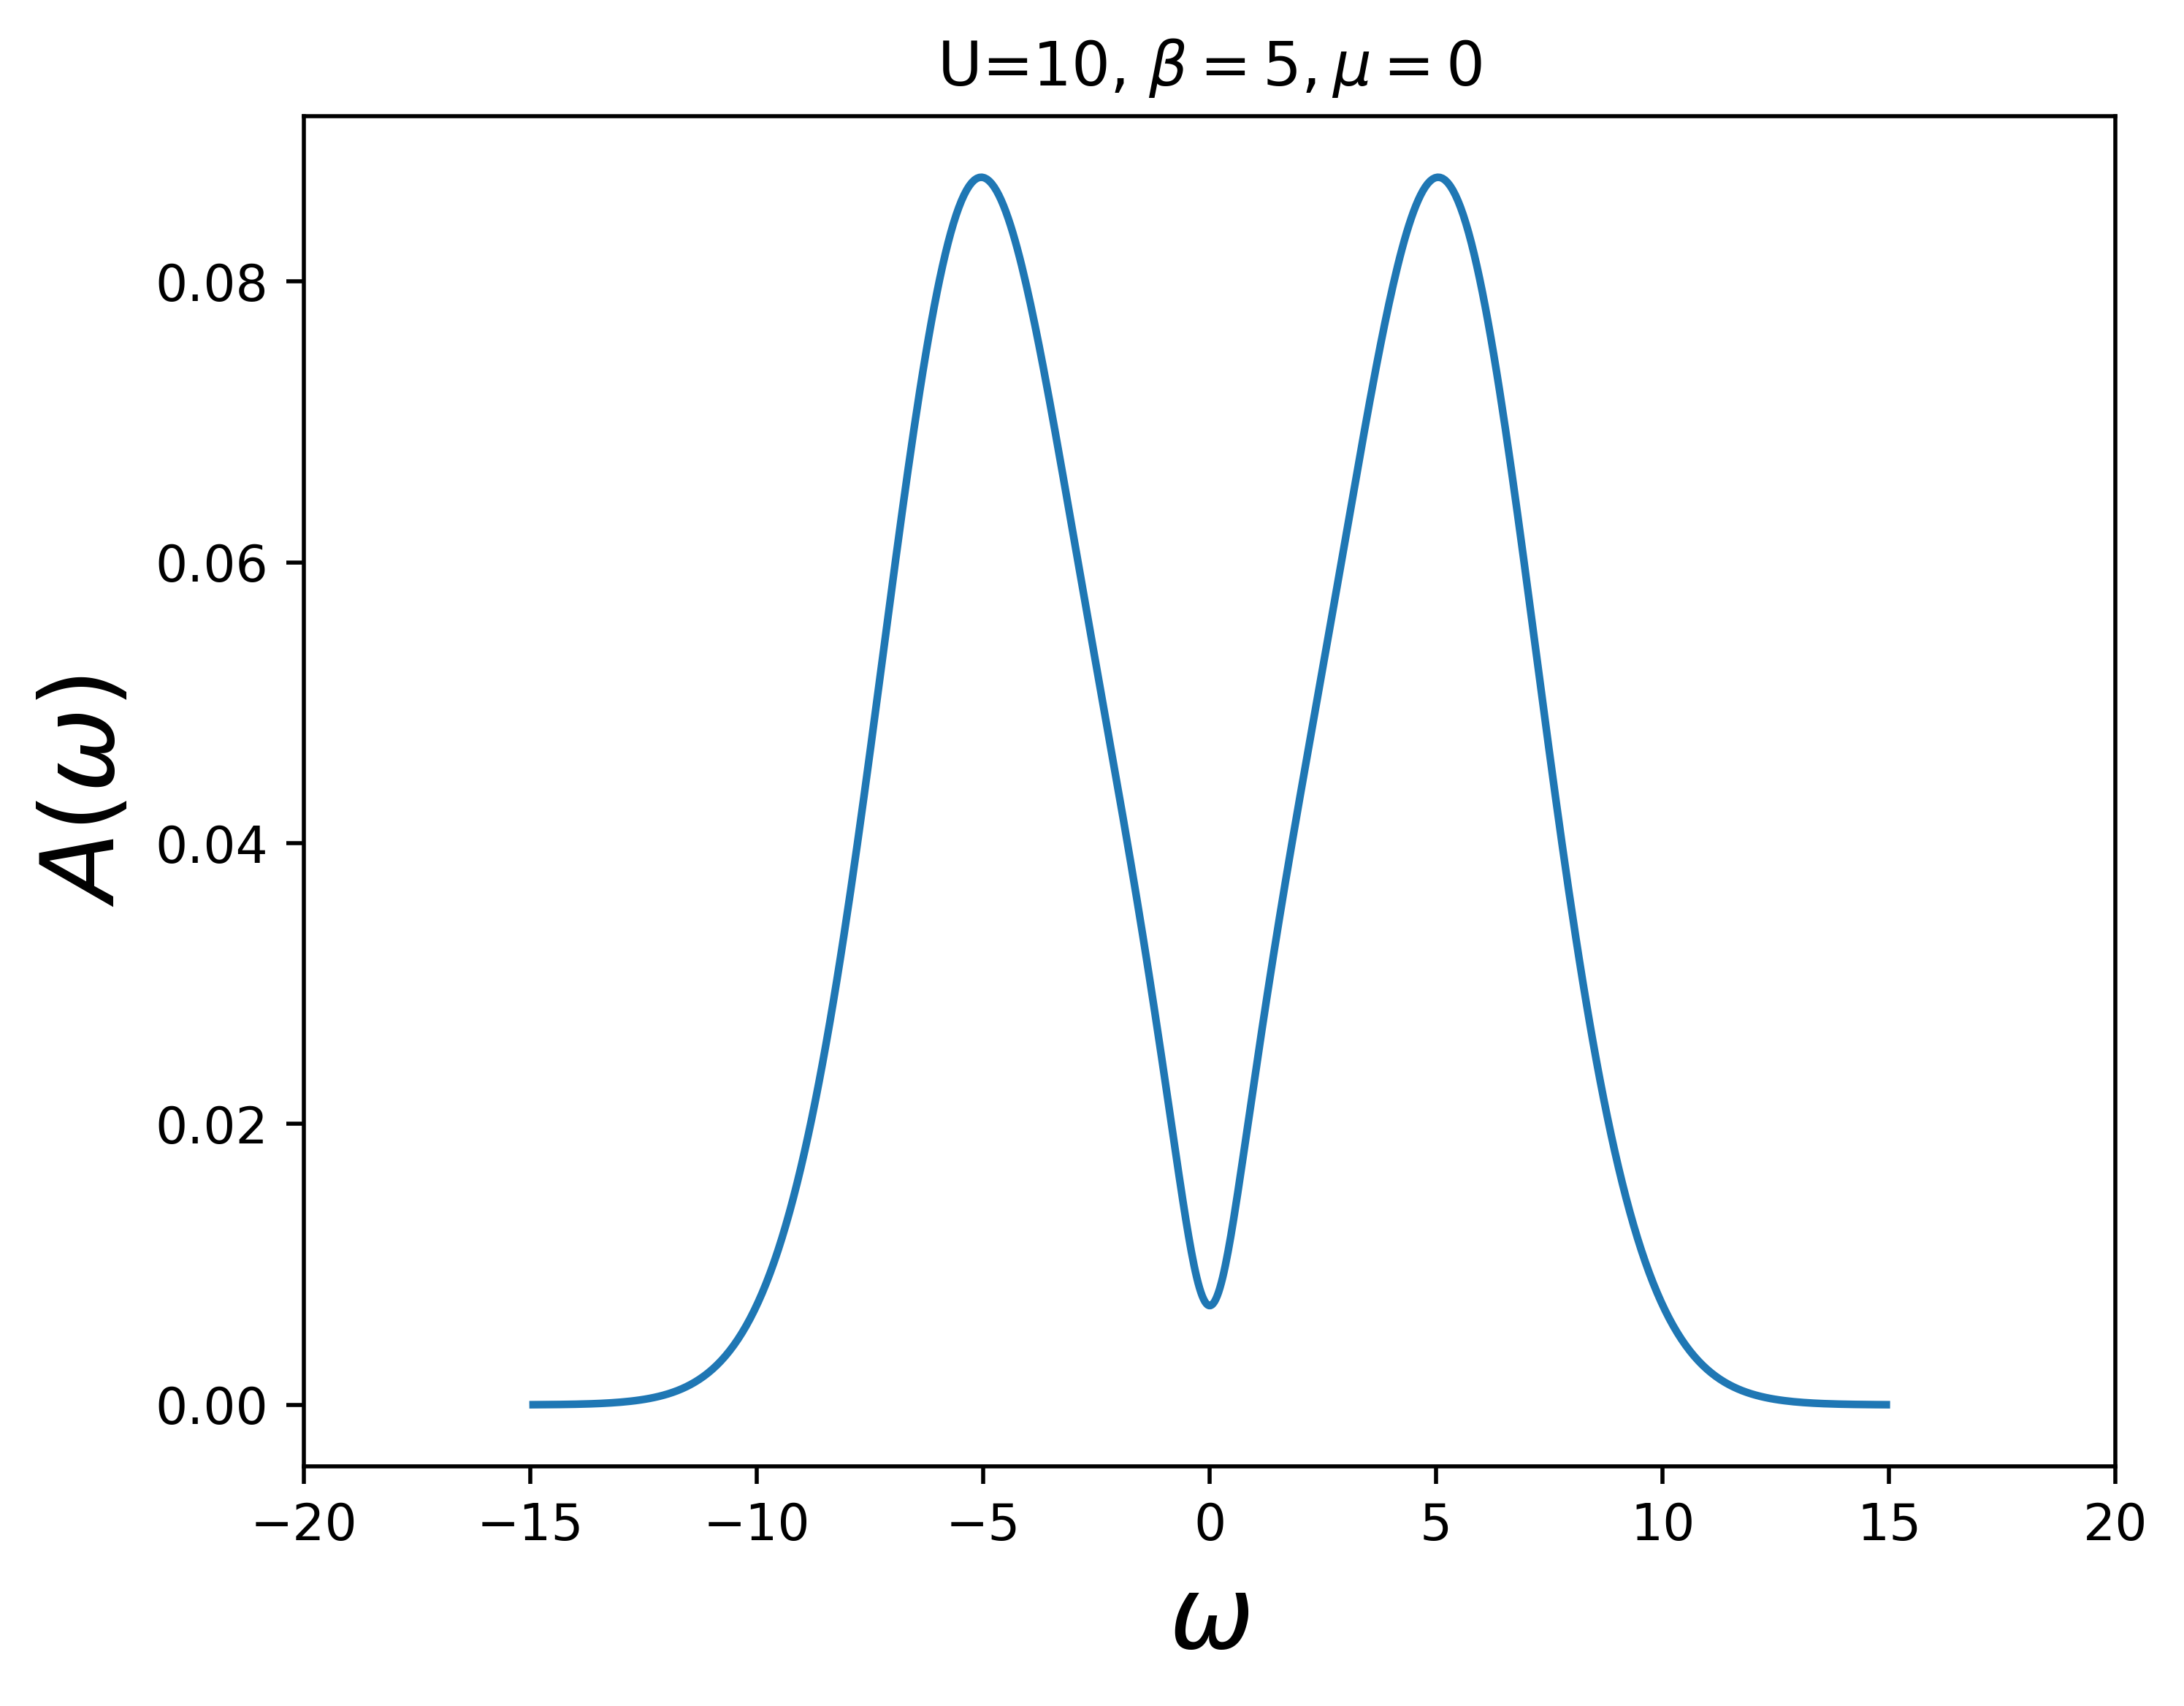
\includegraphics[width=0.45\linewidth]{fig2/spectral10.png}
         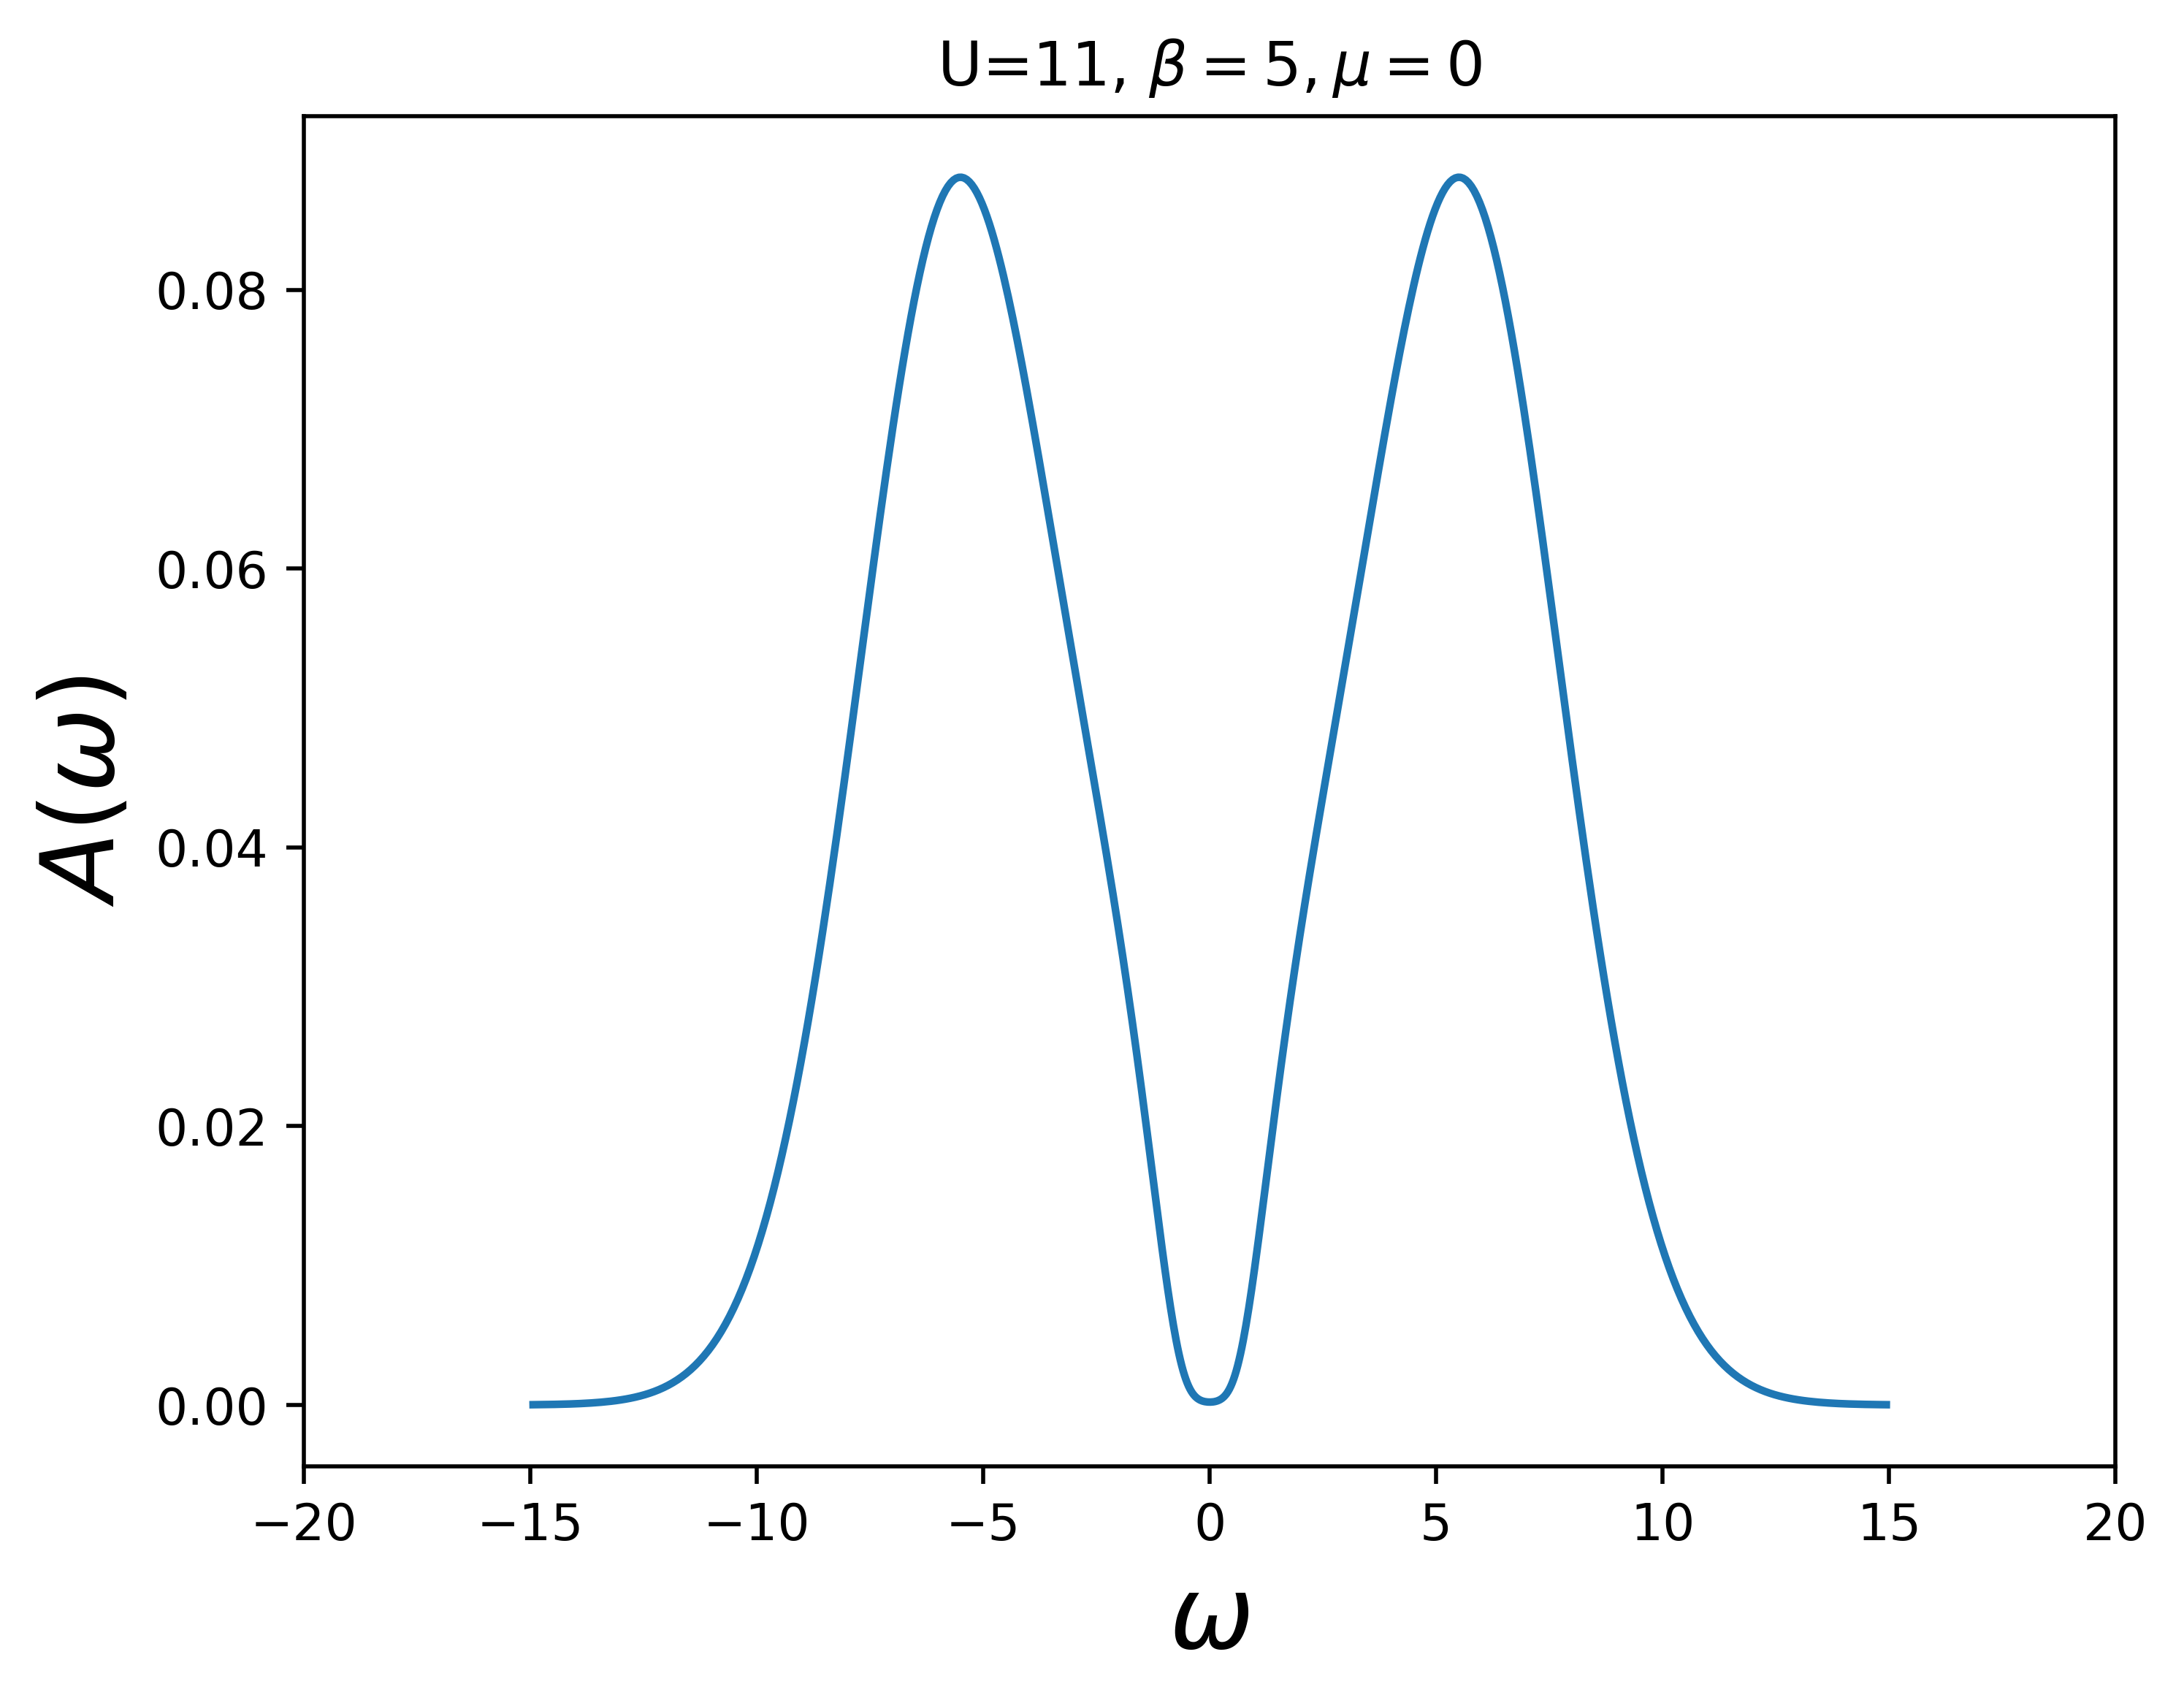
\includegraphics[width=0.45\linewidth]{fig2/spectral11.png}
          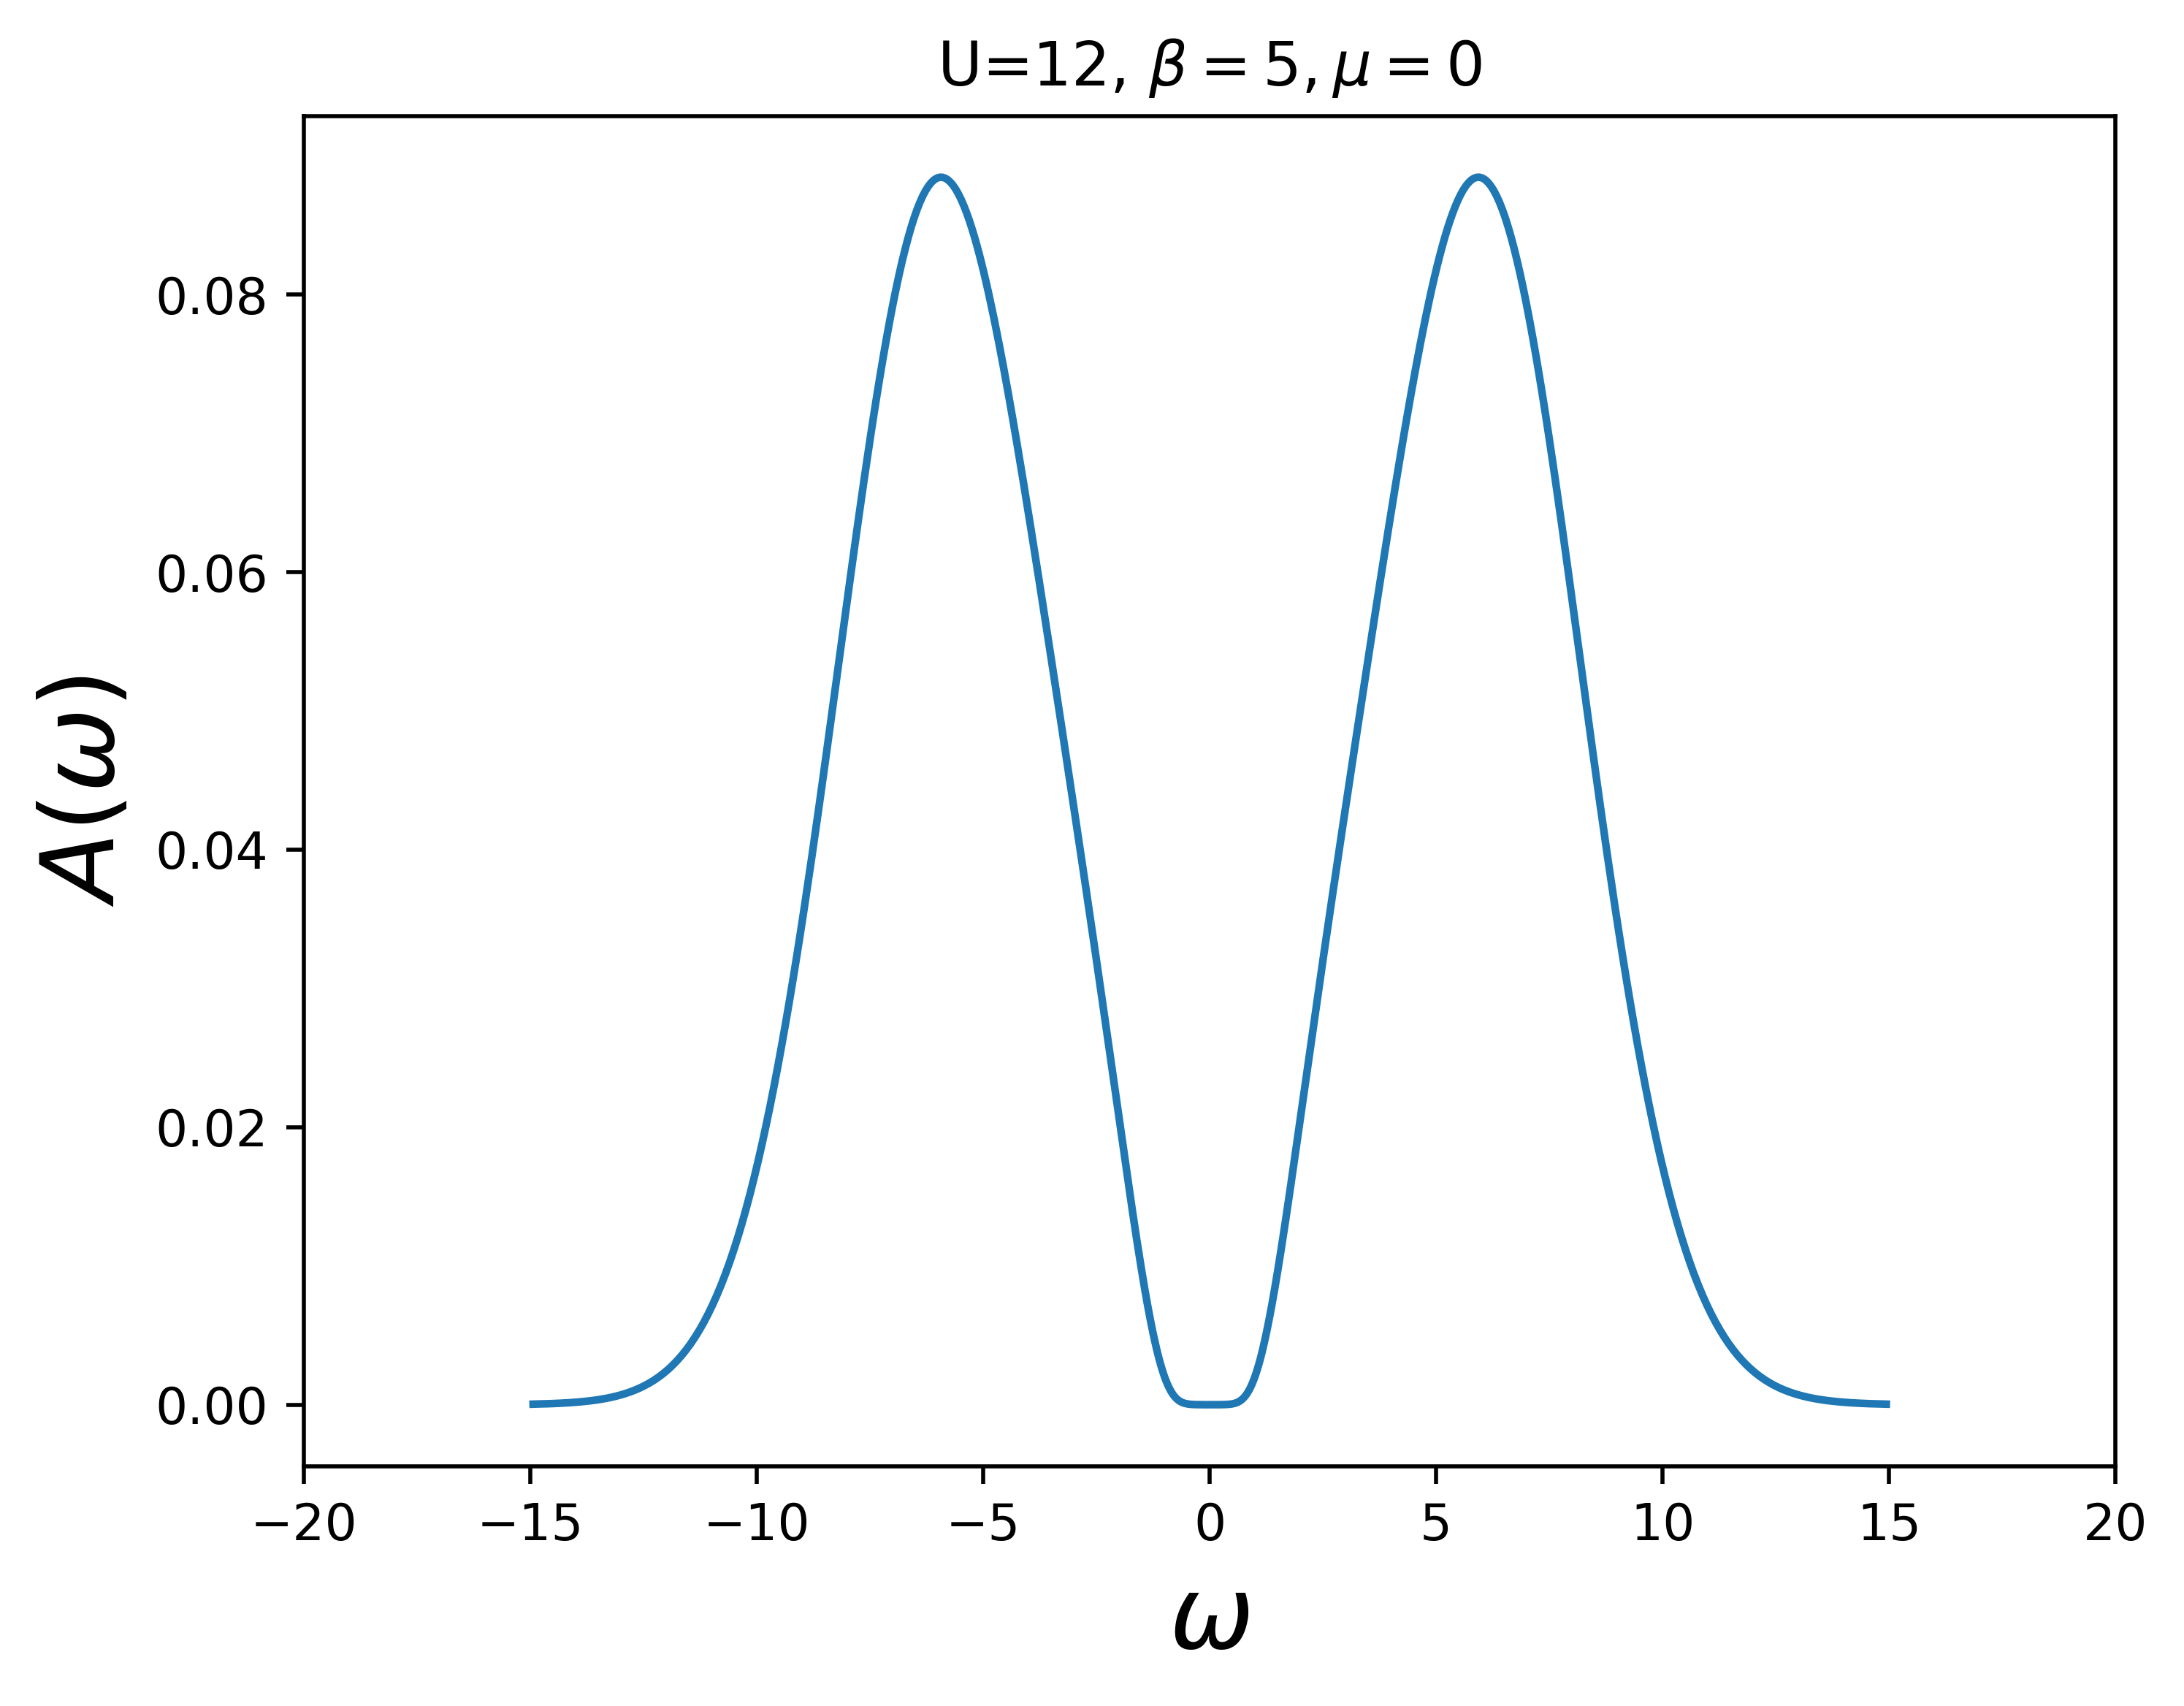
\includegraphics[width=0.45\linewidth]{fig2/spectral12.png}
           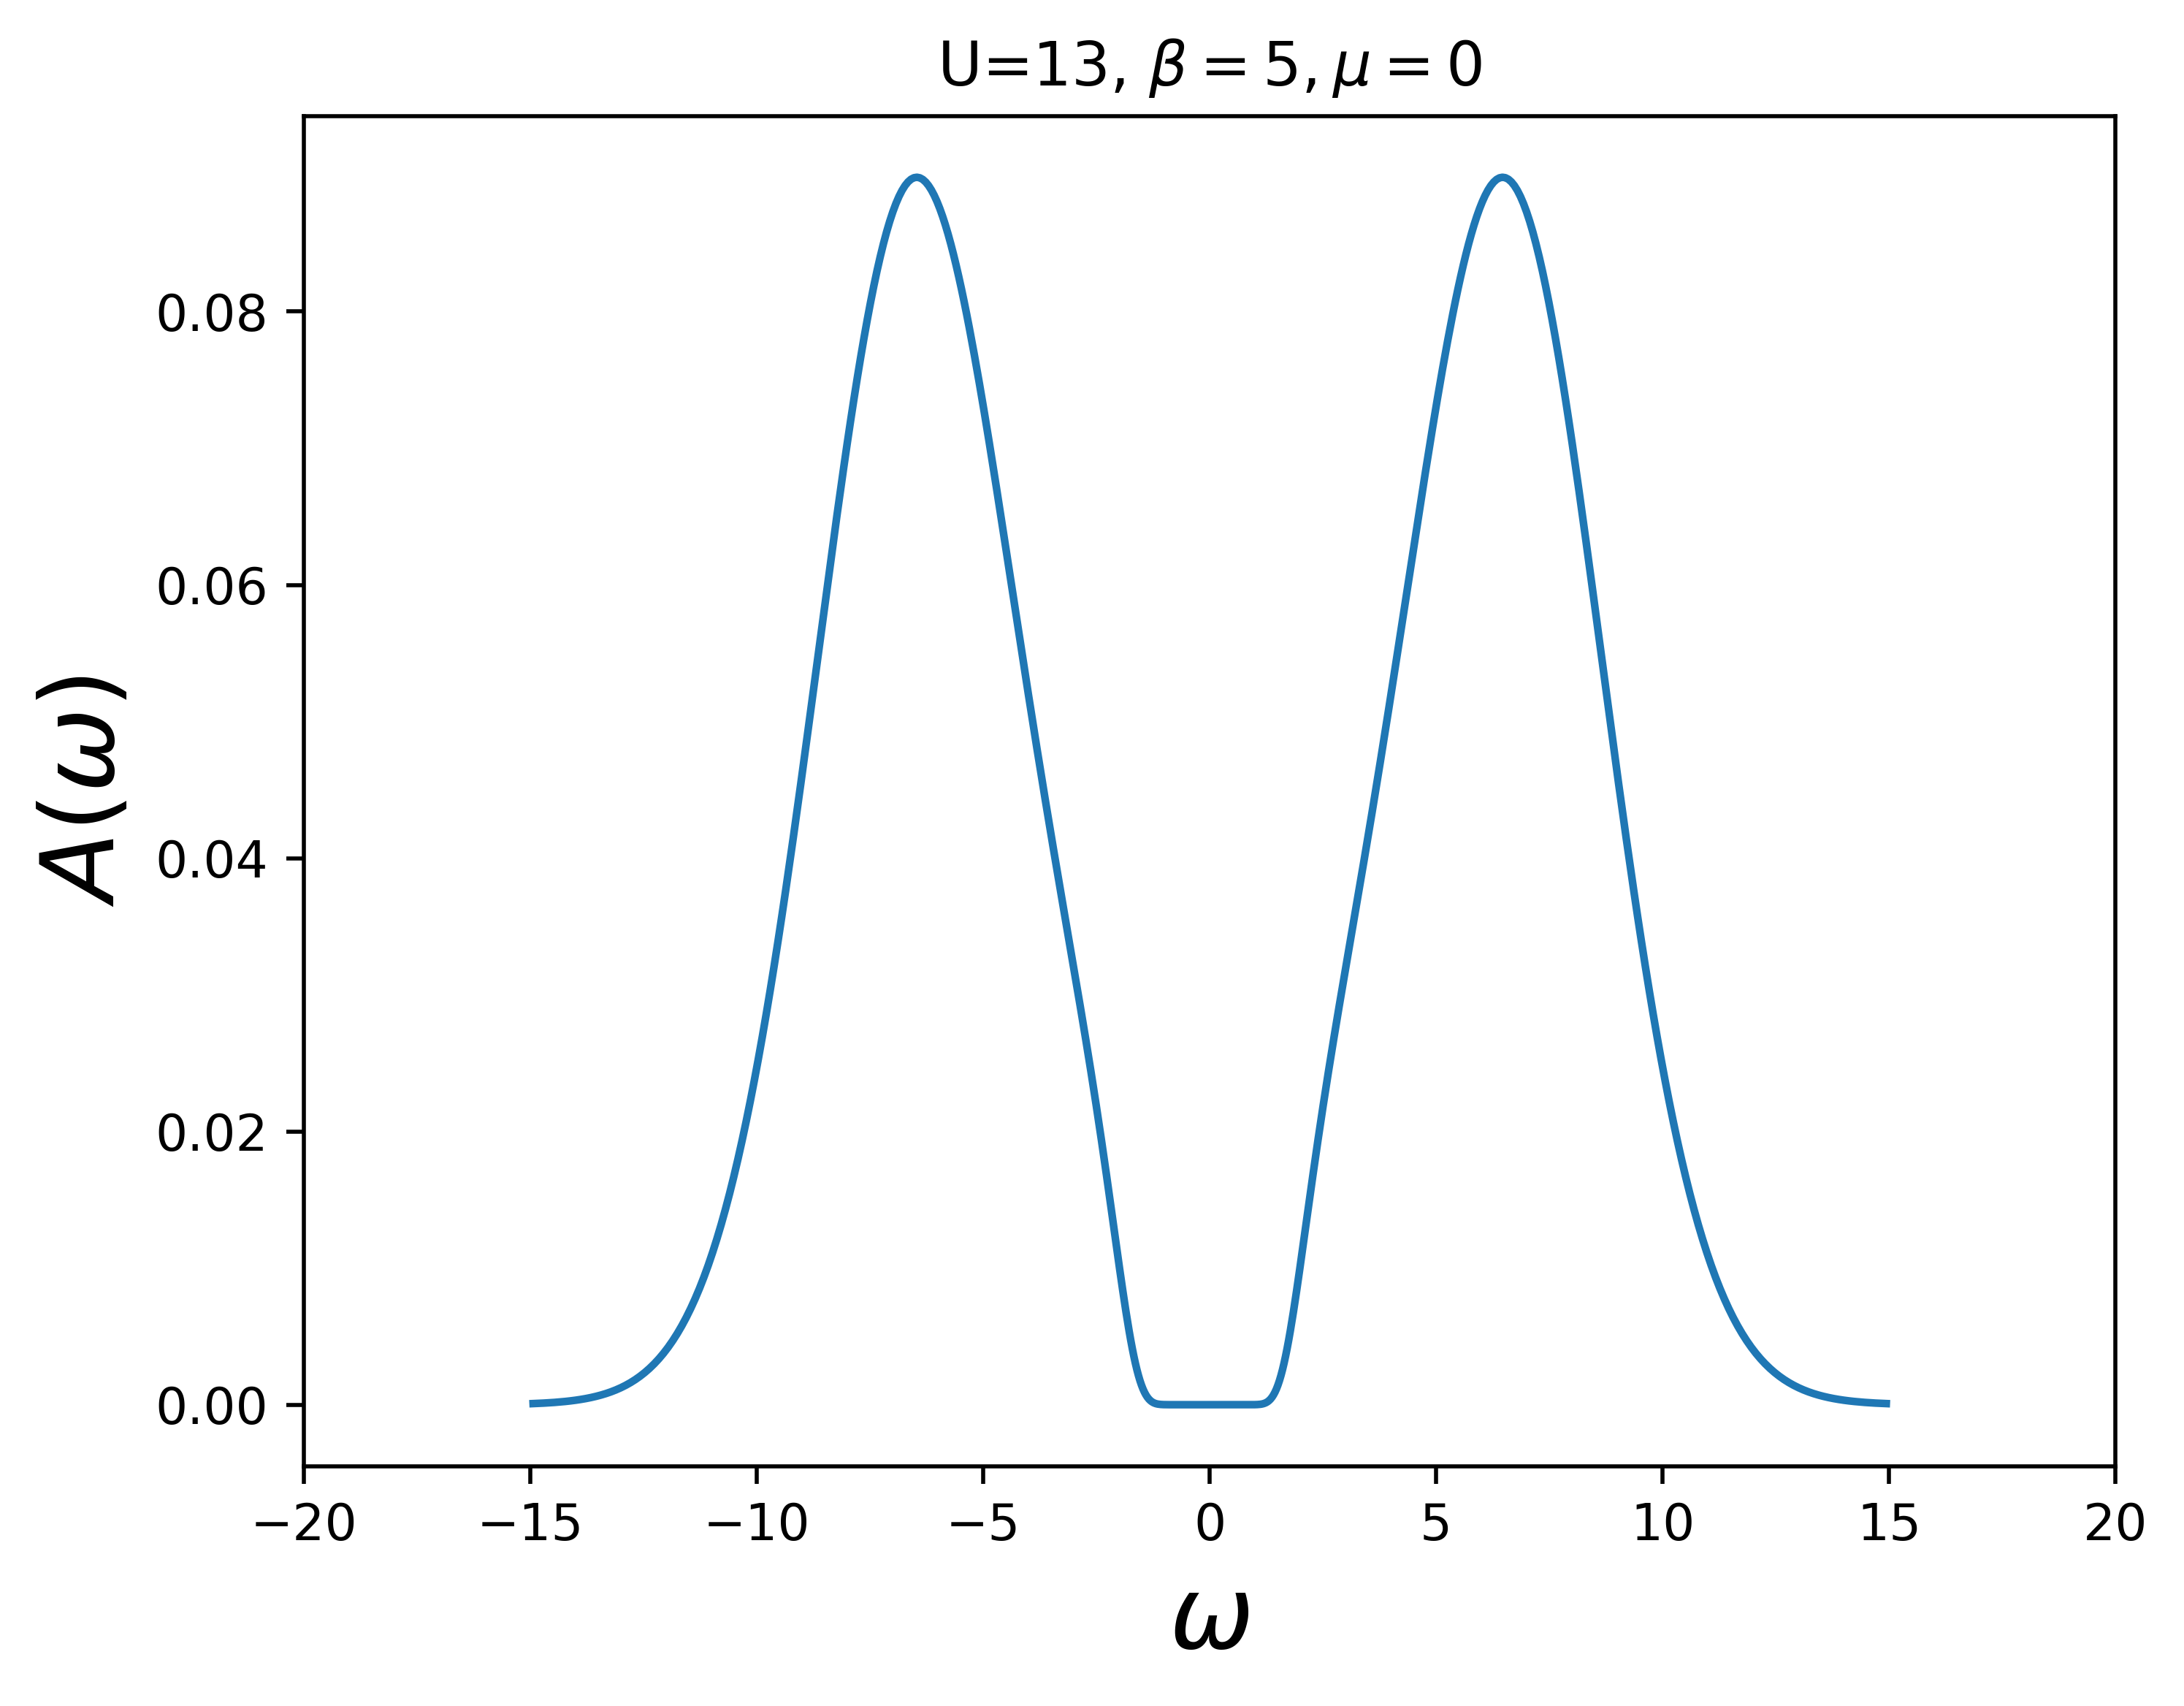
\includegraphics[width=0.45\linewidth]{fig2/spectral13.png}
\caption{ Spectral function $A(\omega)$, output of Maxent from DMFT results for $U=3$ to $U=13$. Transition from Fermi liquid state to non-Fermi liquid state can be seen, gap appears at $U=12$. \label{fig:DMFT_spectral}}
\vspace{-20pt}
\end{figure} 


\begin{figure}[ht]
\centering
    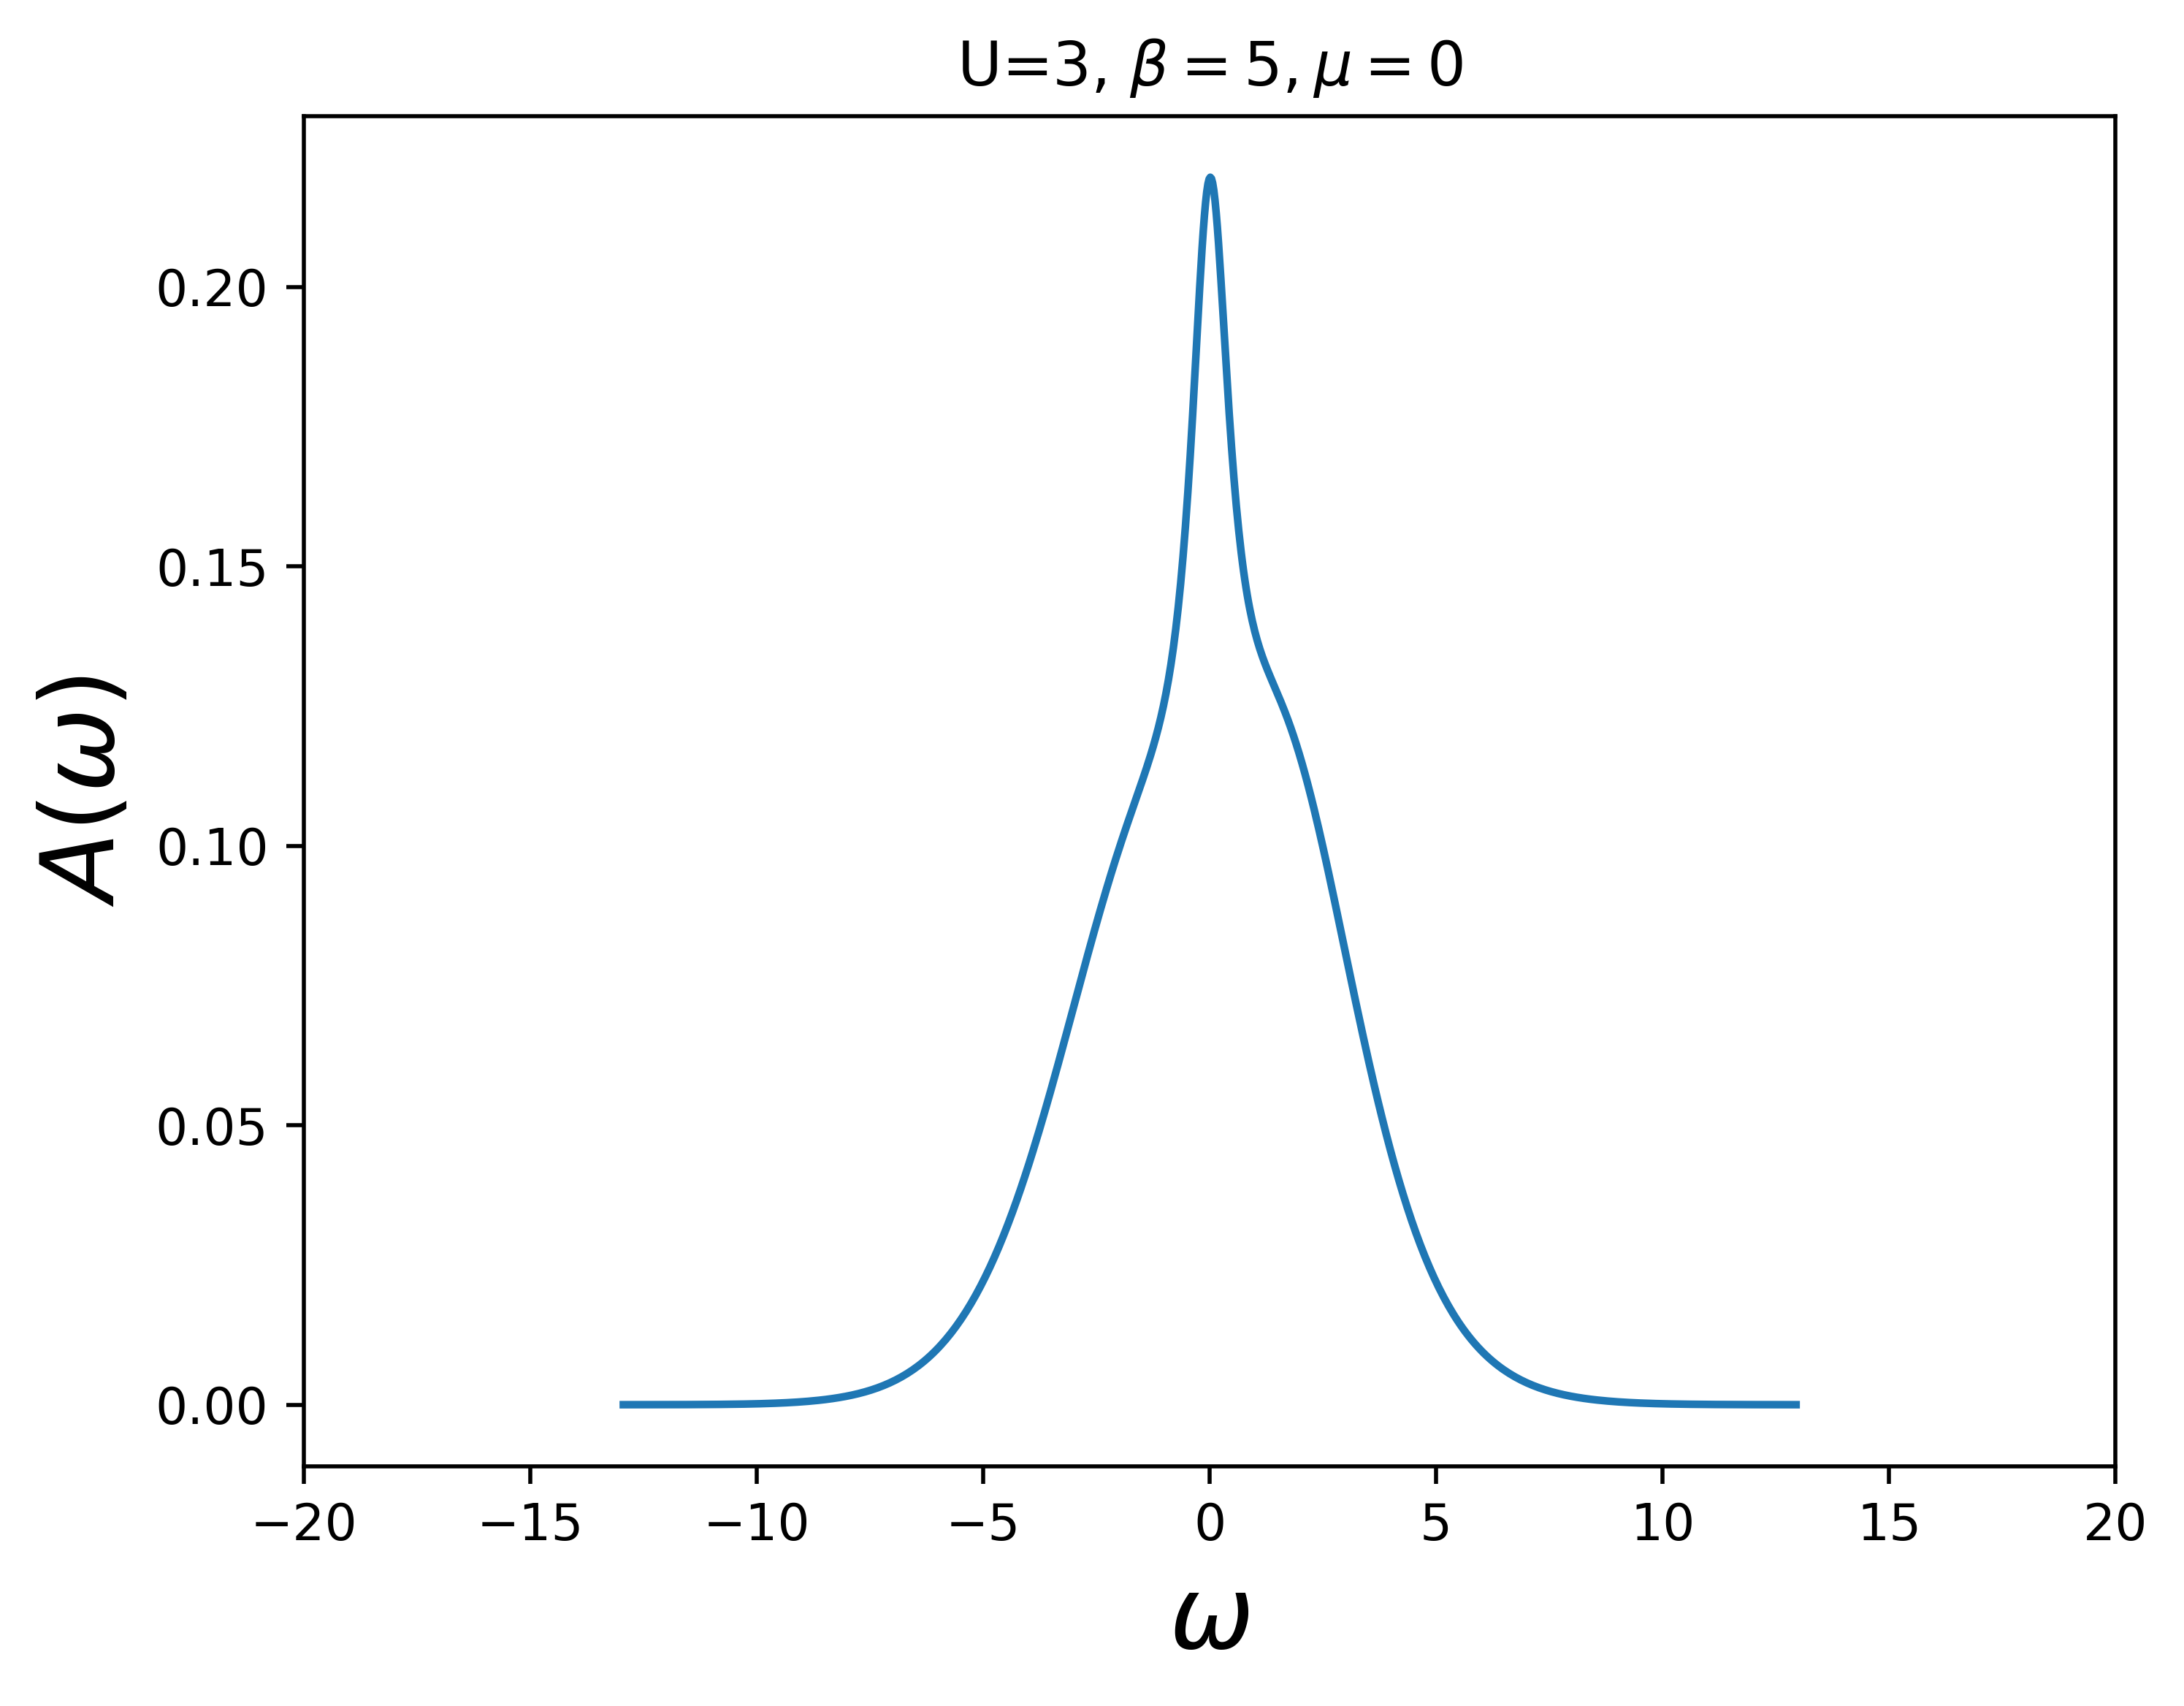
\includegraphics[width=0.45\linewidth]{fig2/dfspectral3.png}
    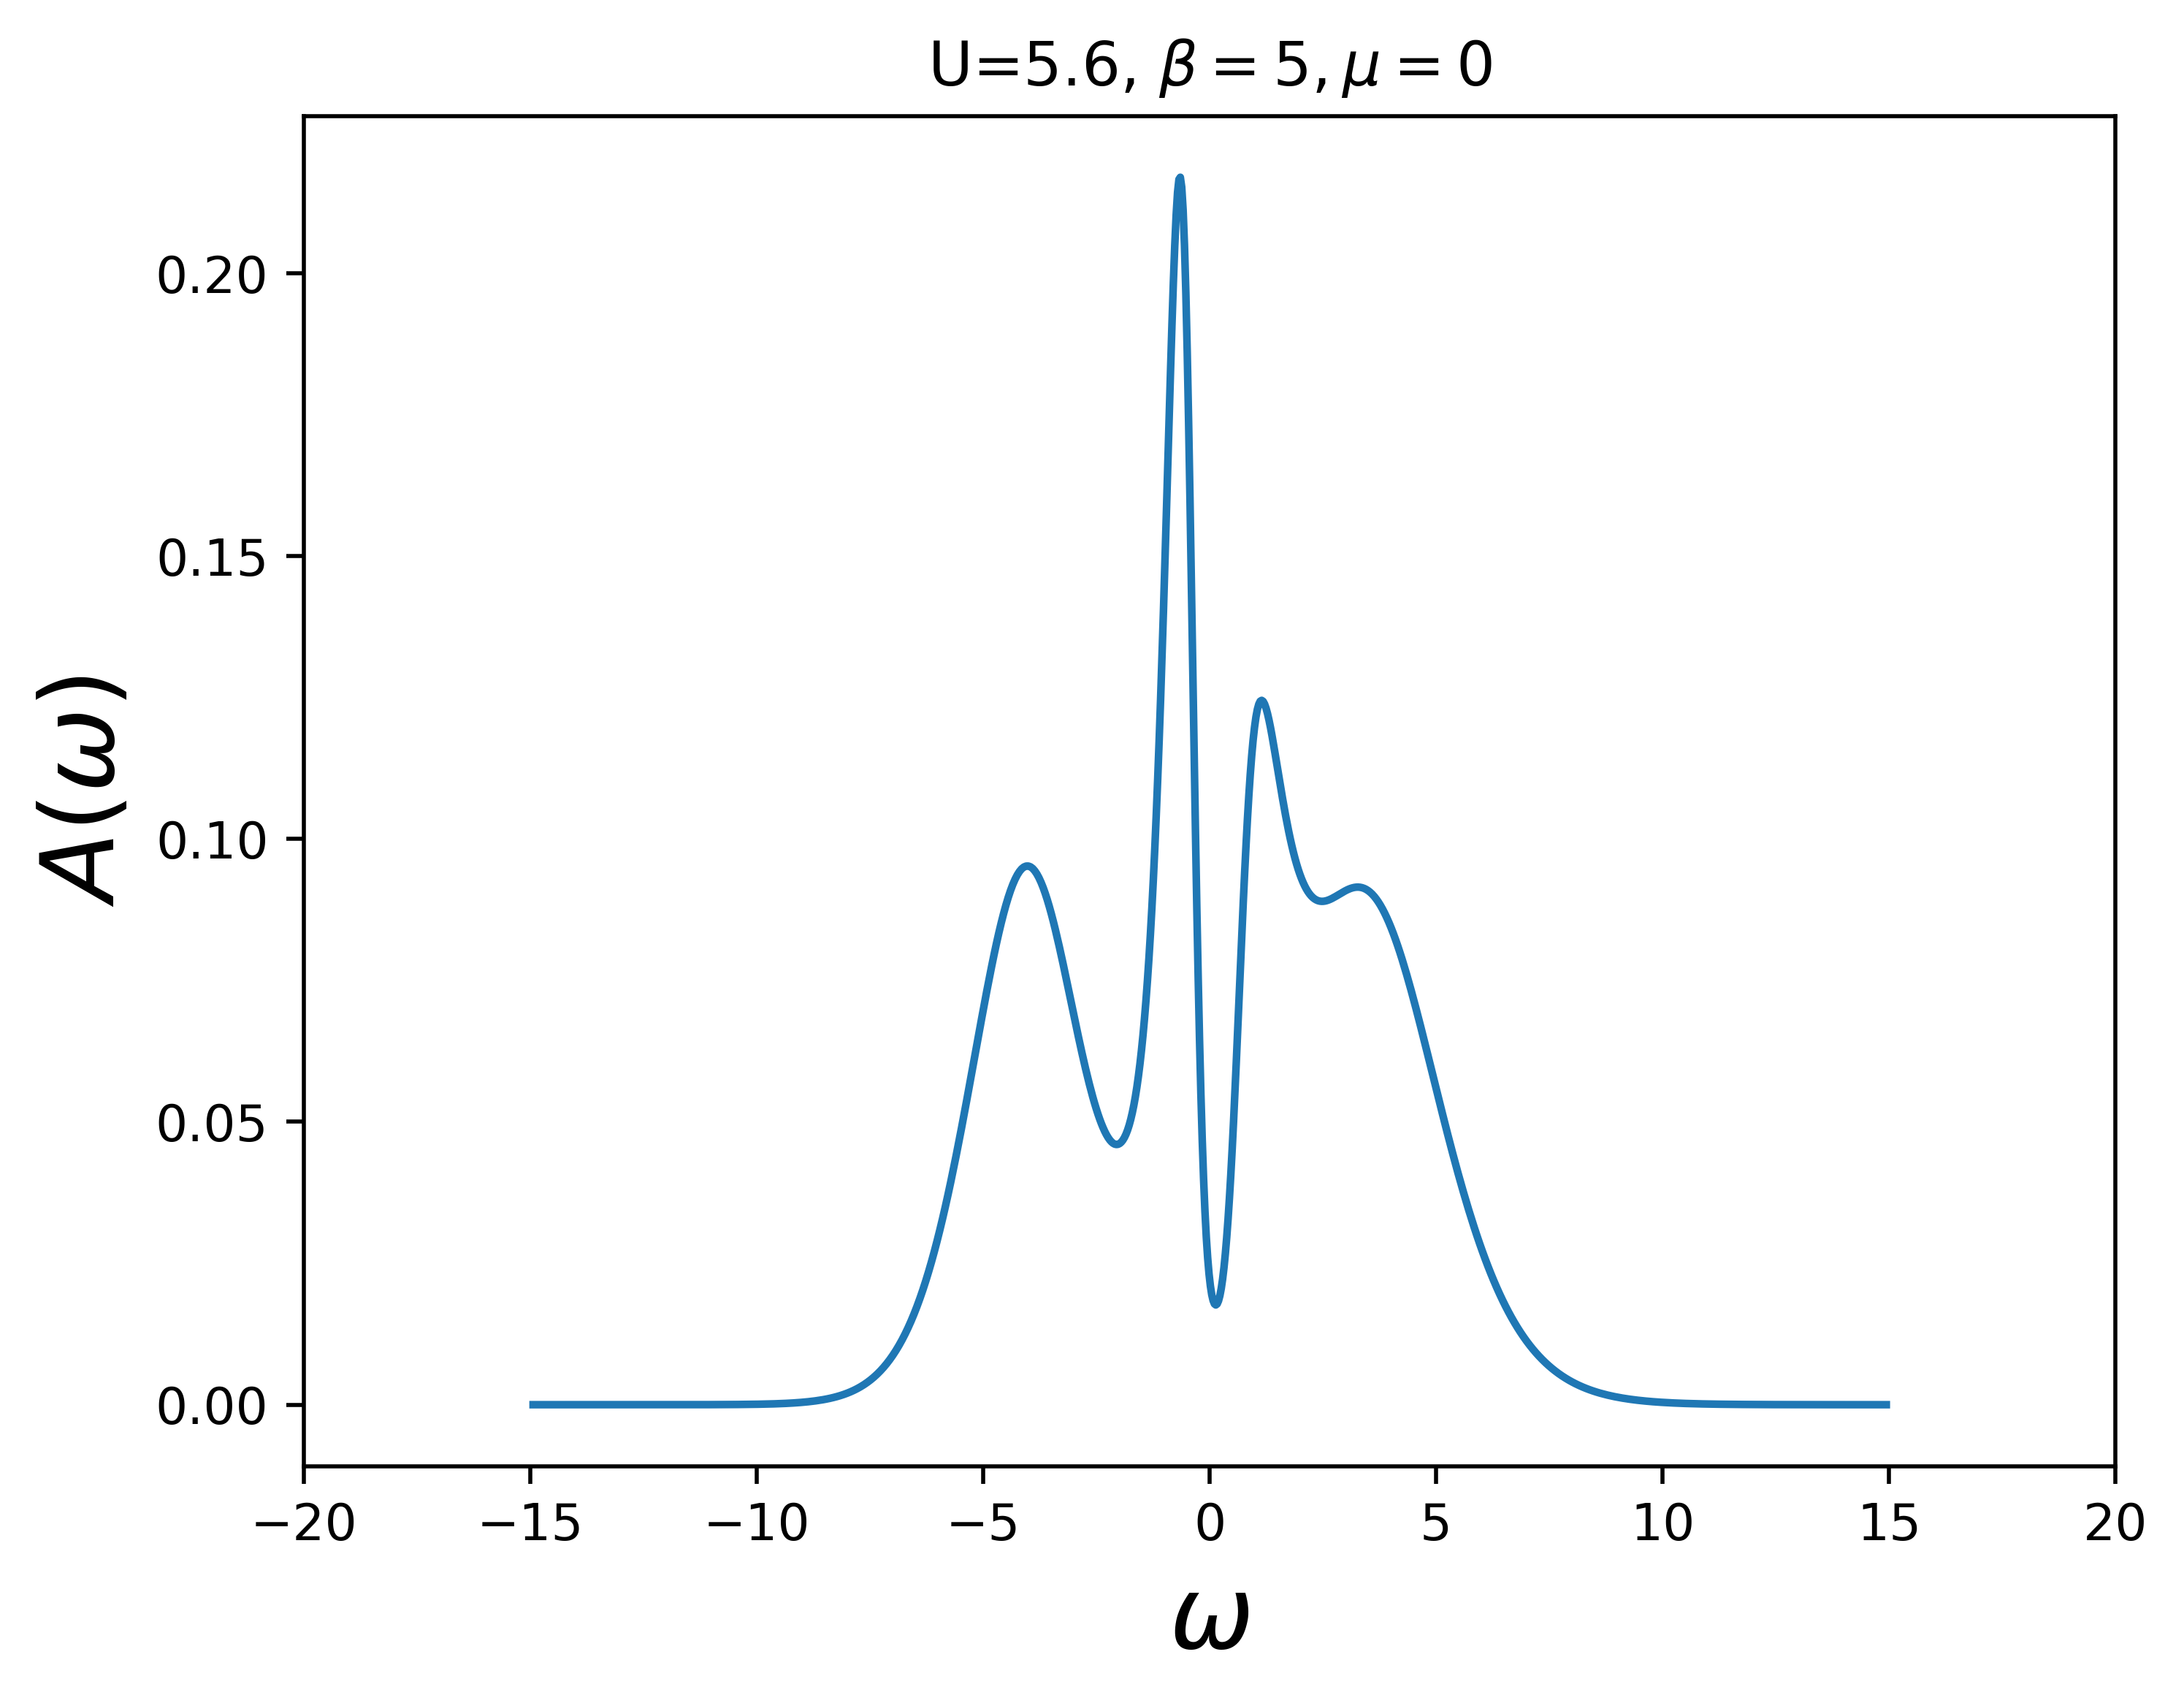
\includegraphics[width=0.45\linewidth]{fig2/dfspectral5.png}
    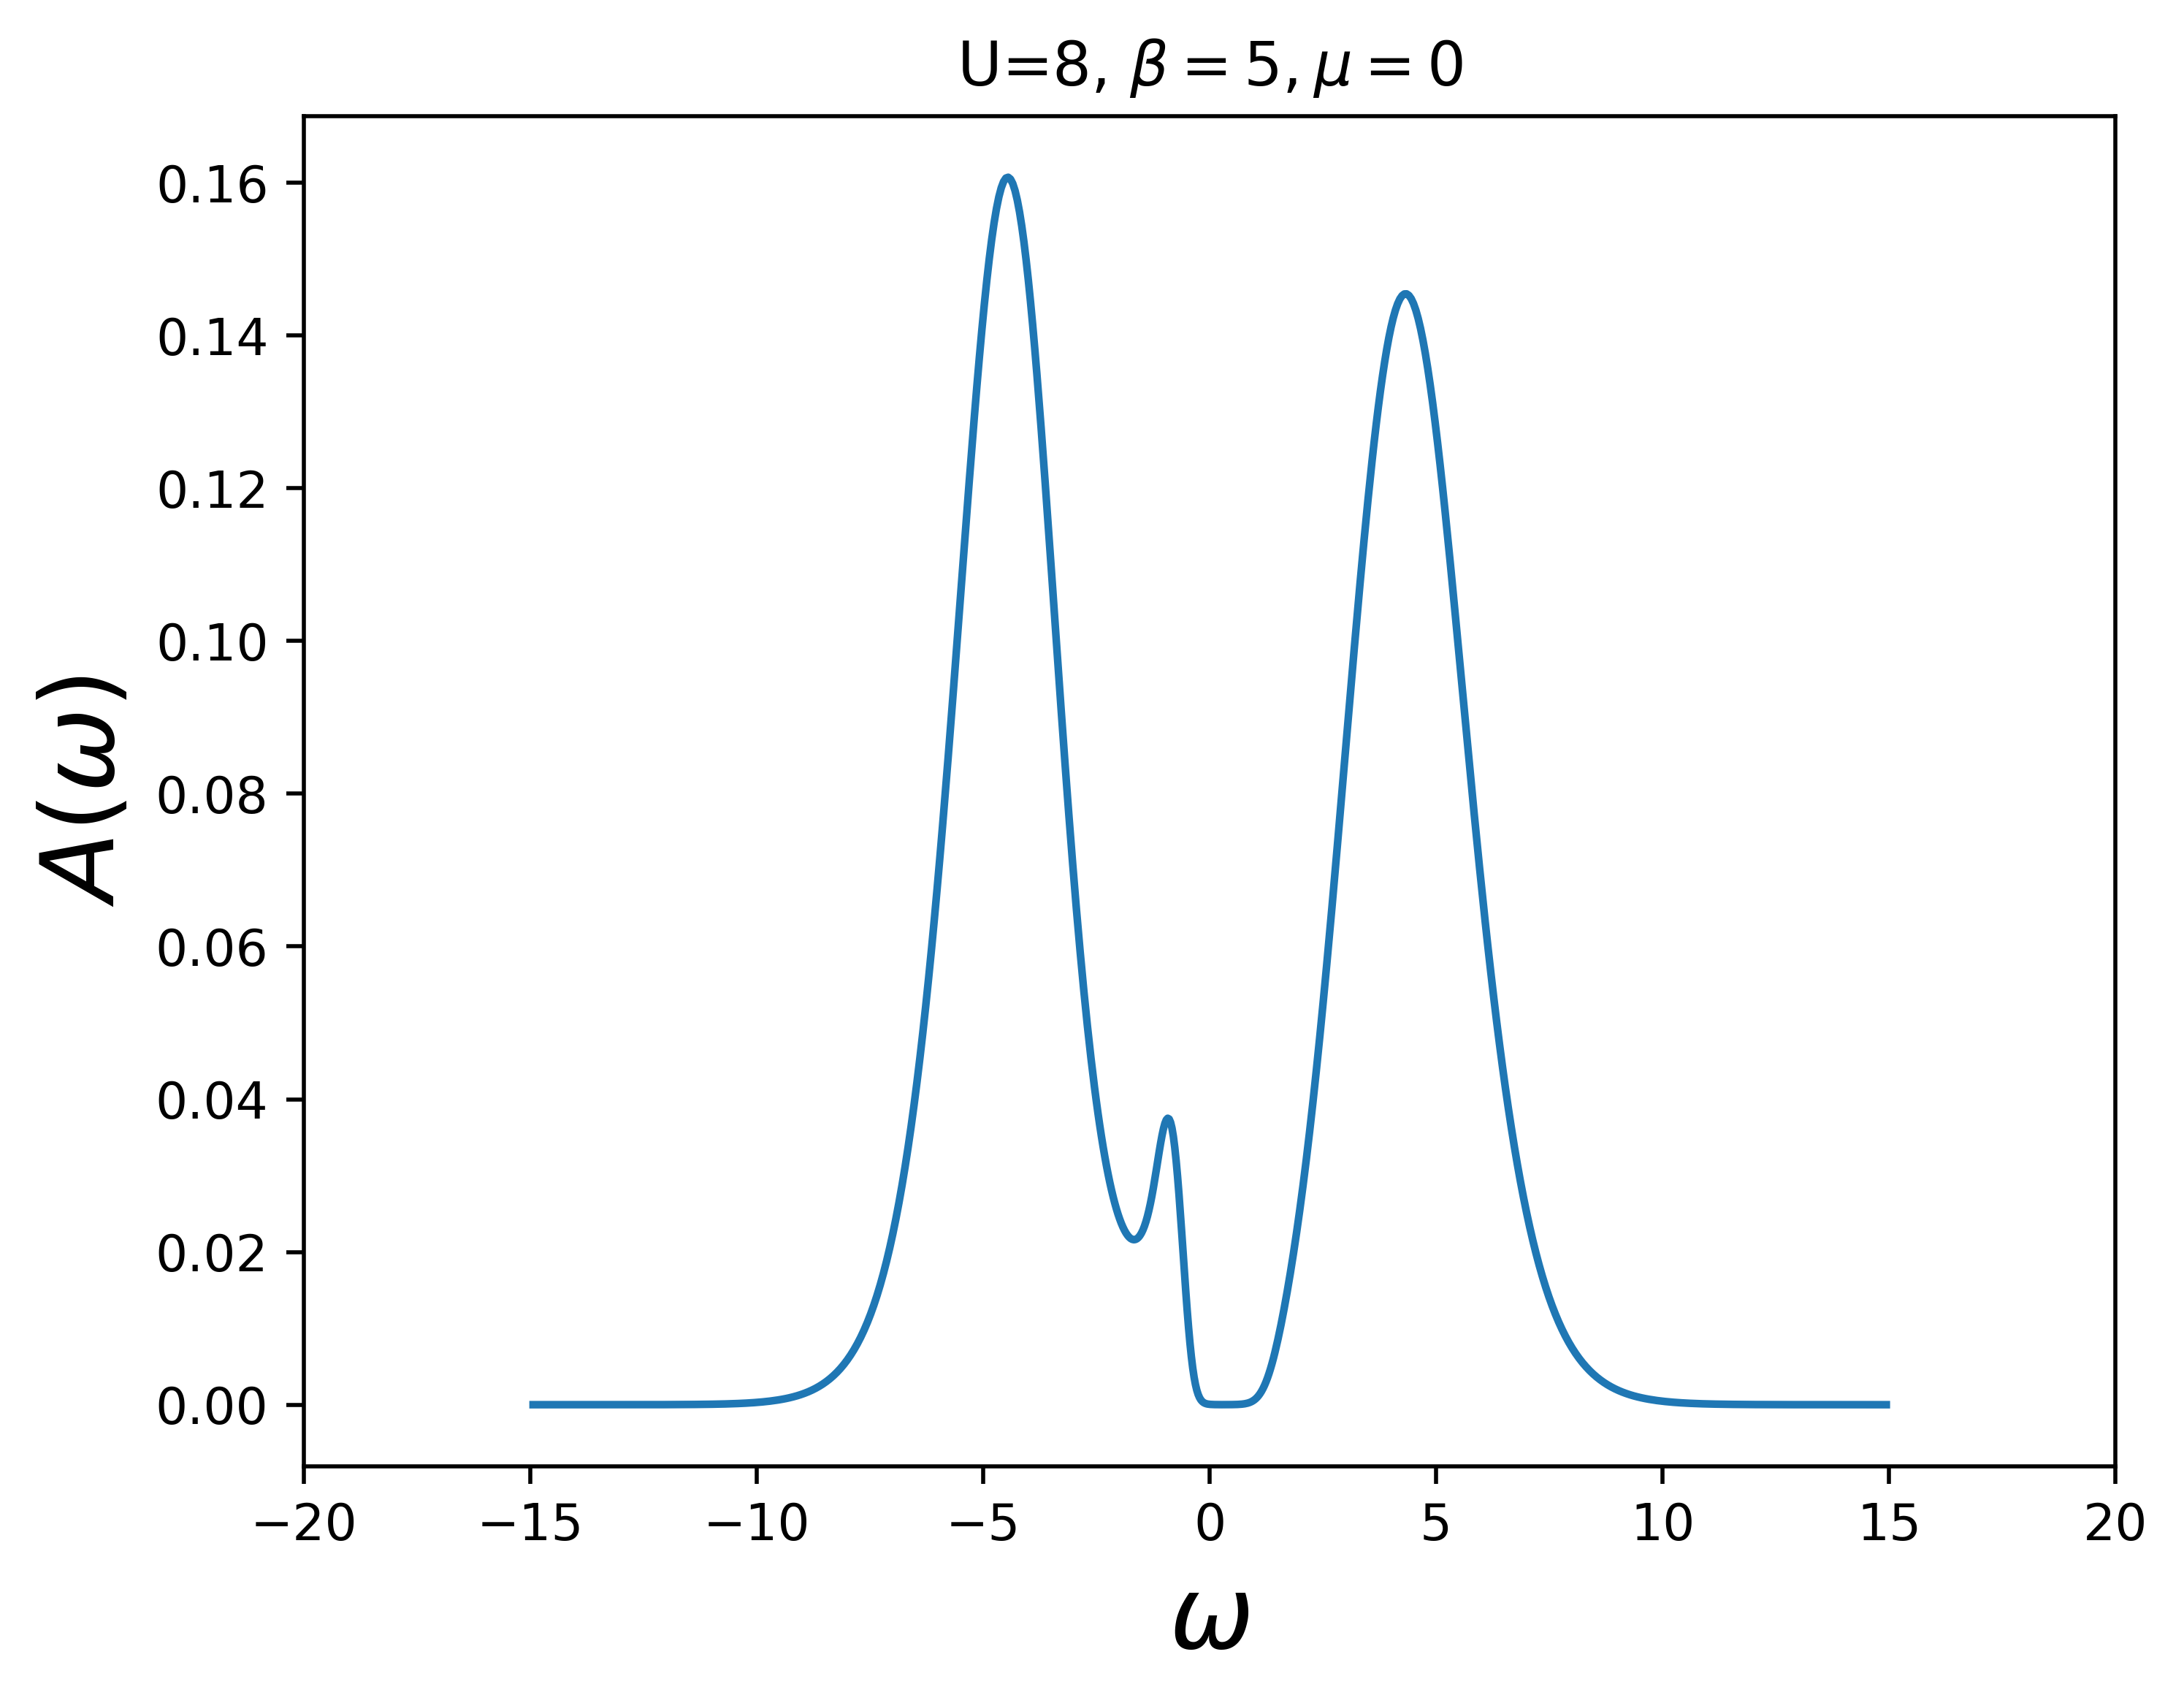
\includegraphics[width=0.45\linewidth]{fig2/dfspectral8.png}
    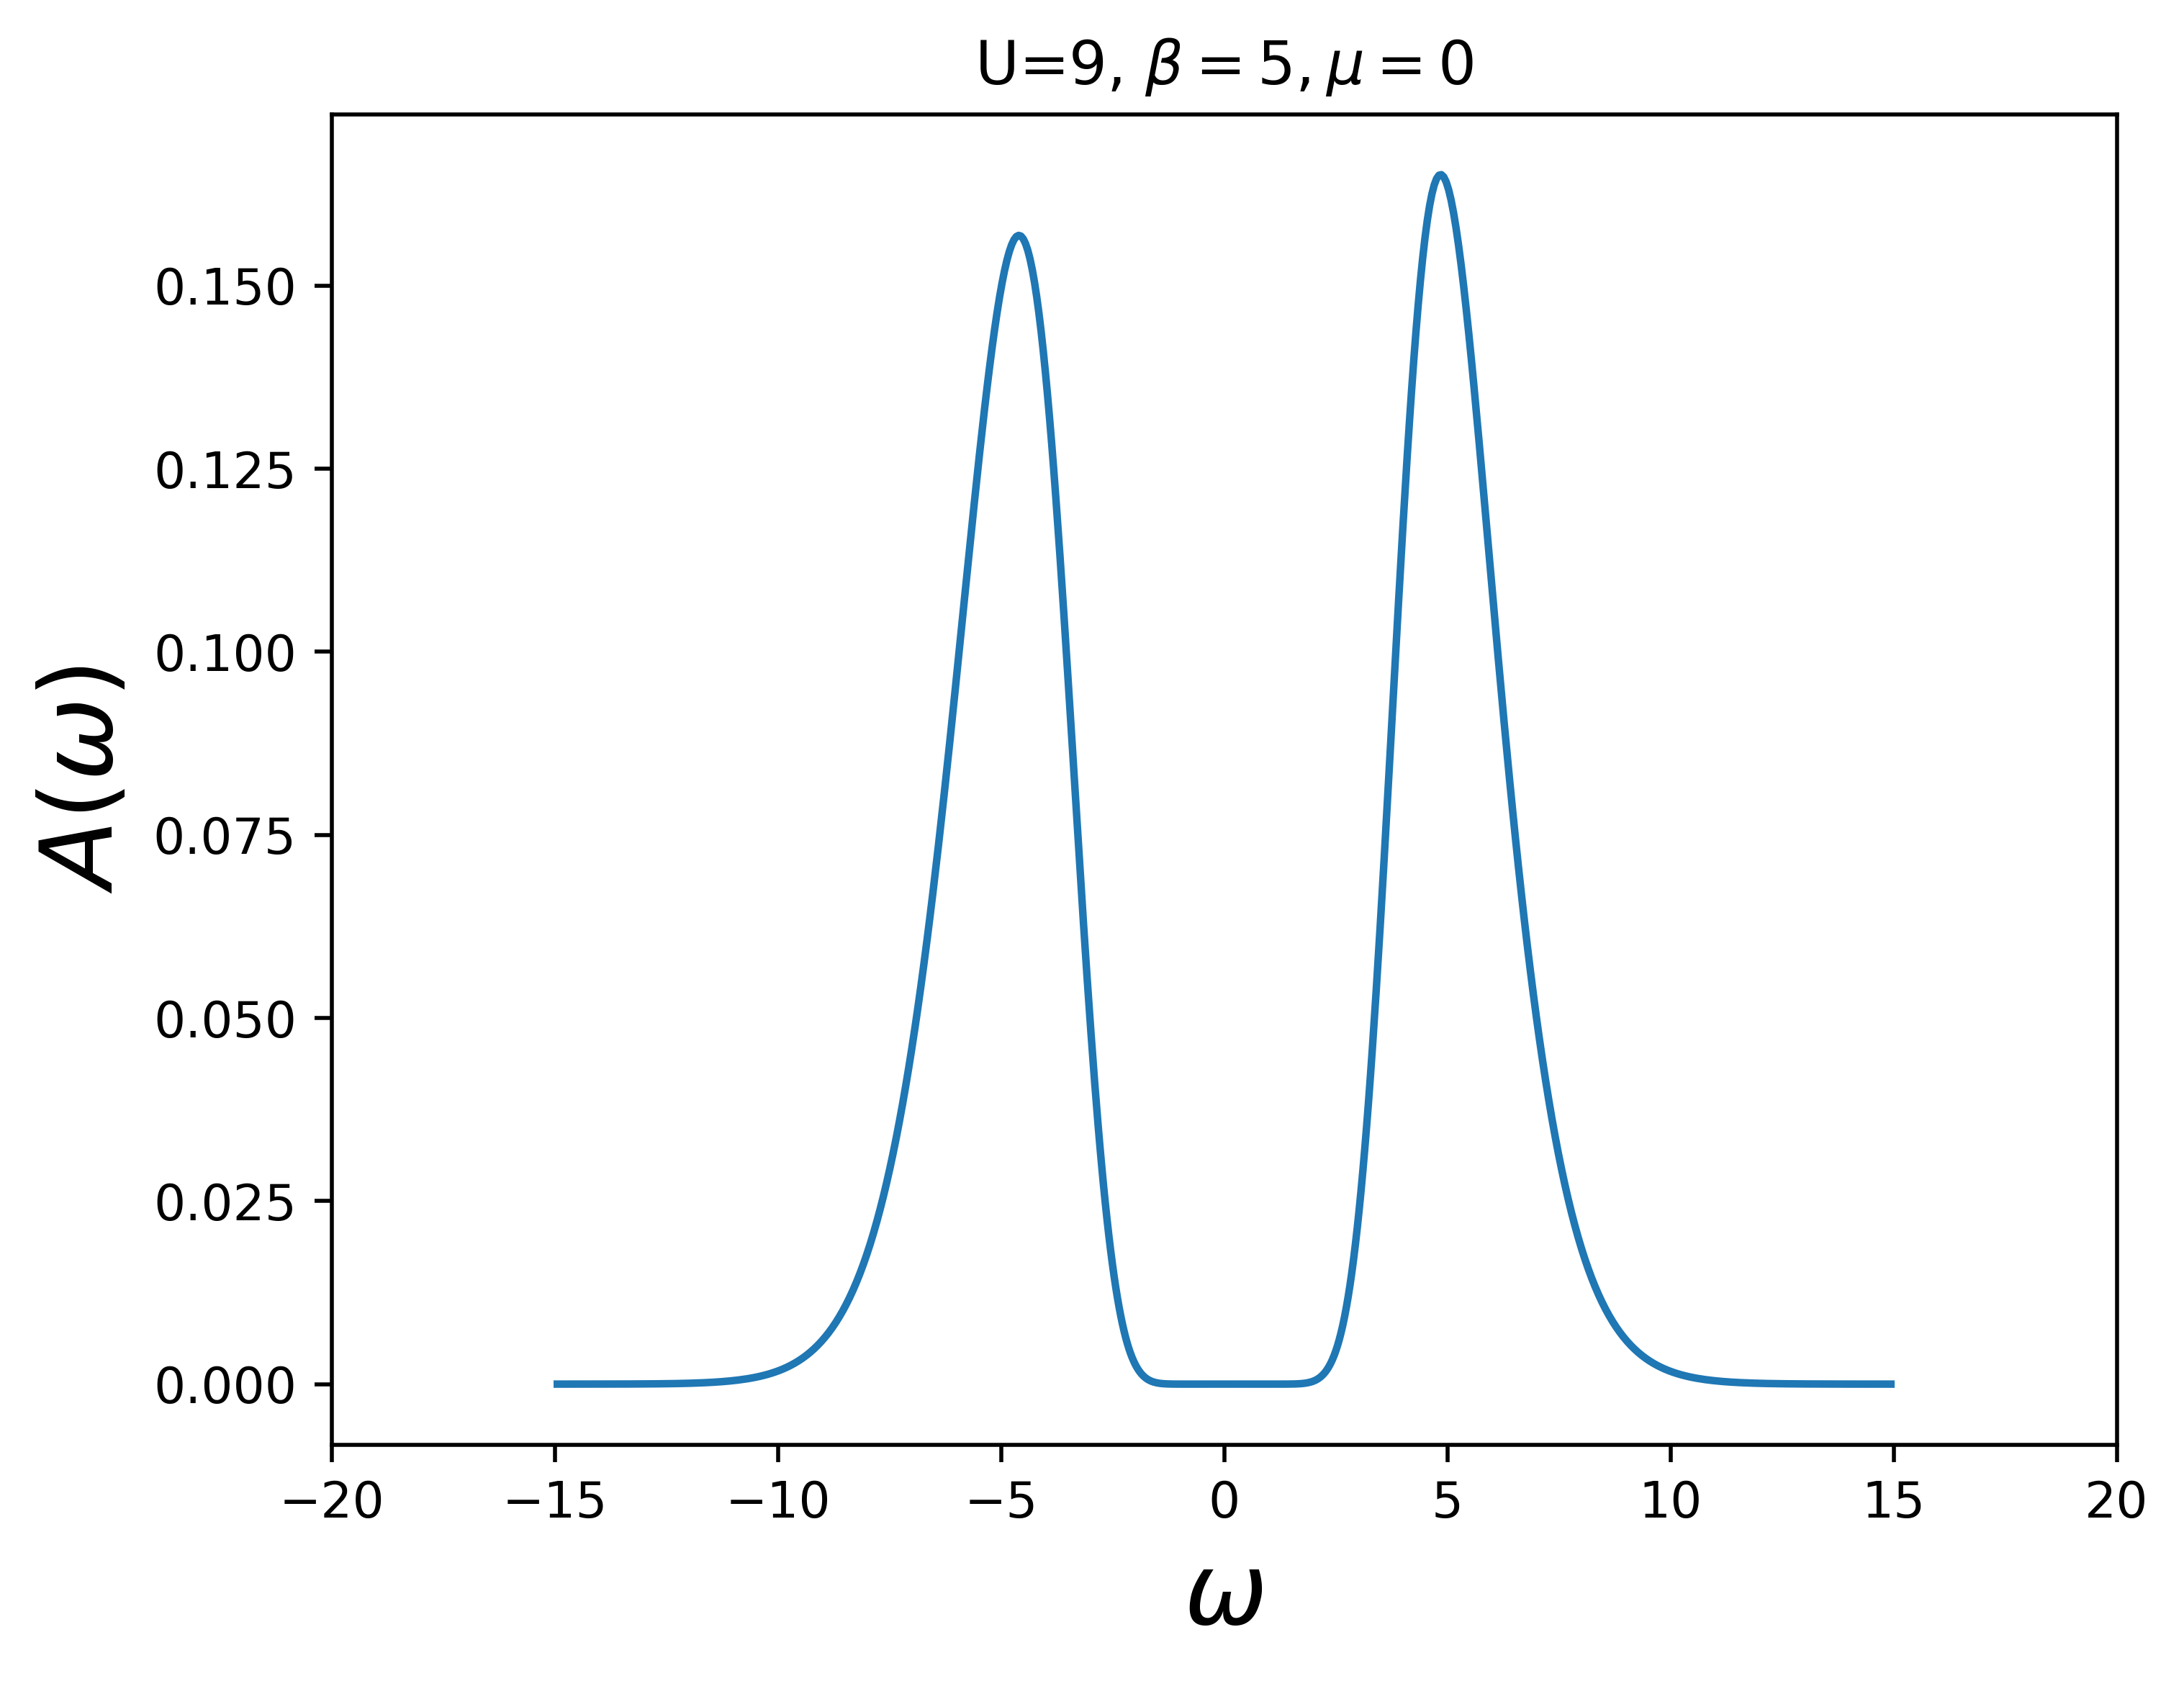
\includegraphics[width=0.45\linewidth]{fig2/dfspectral9.png}
    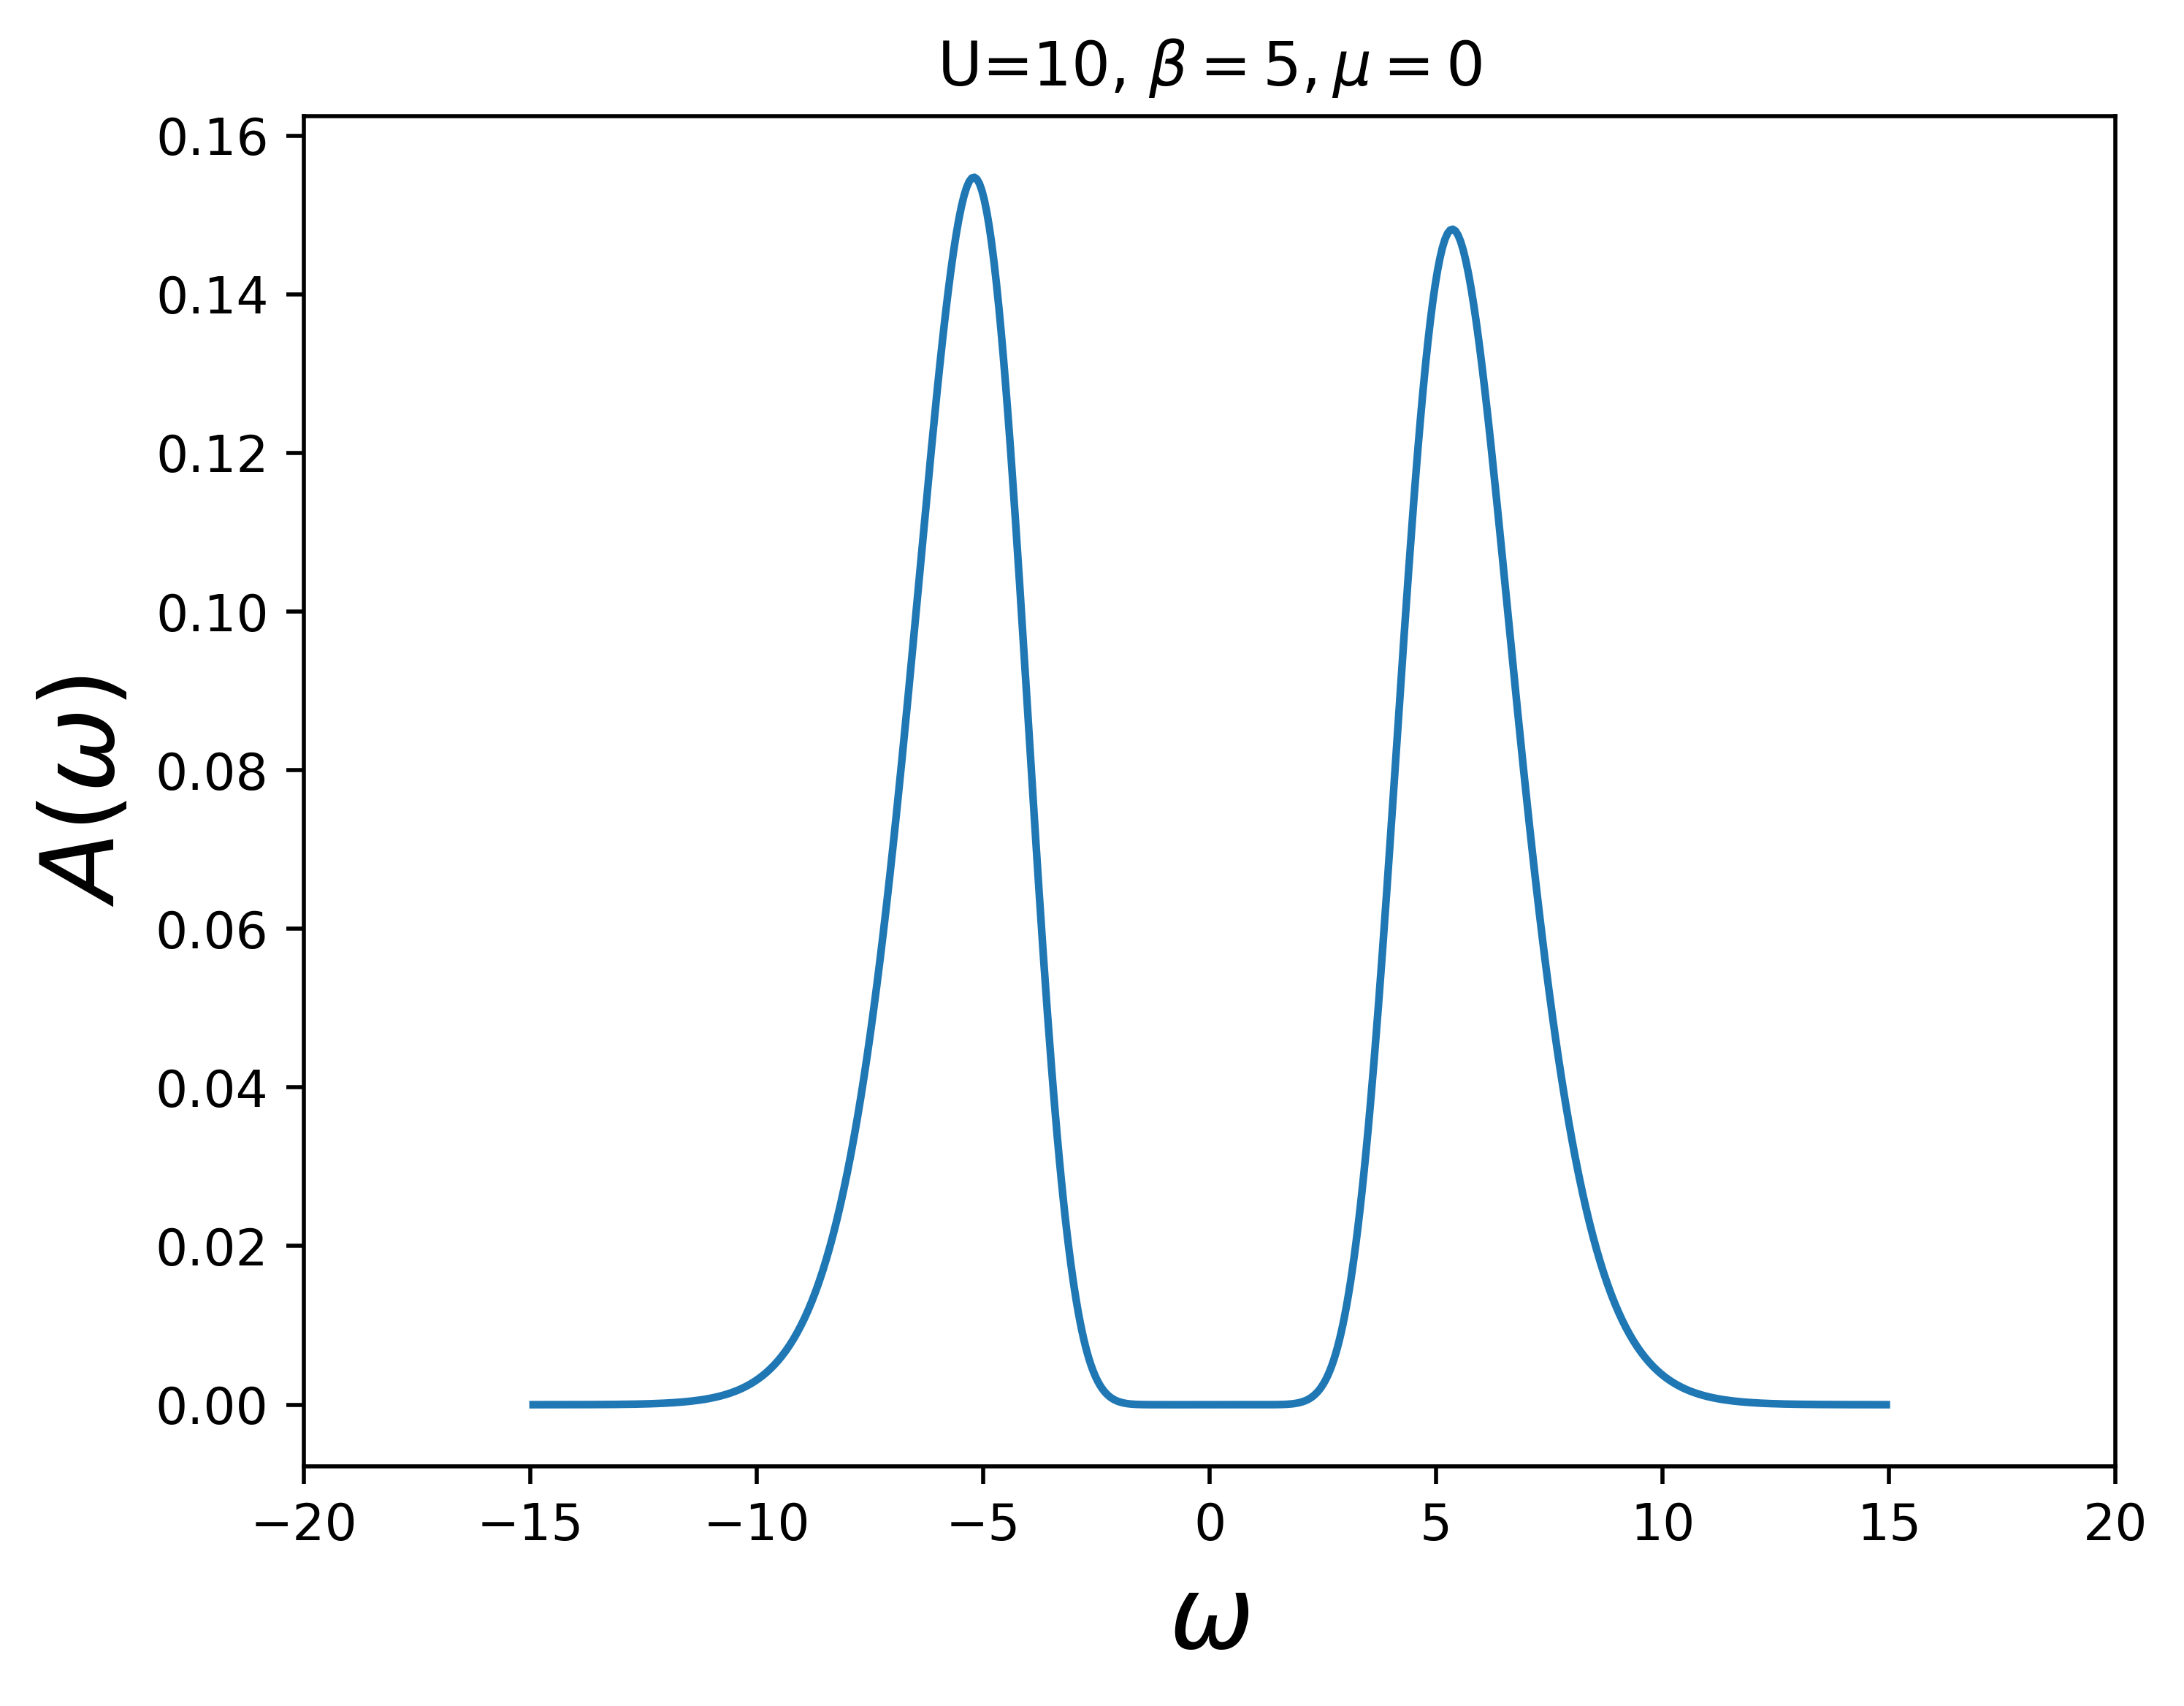
\includegraphics[width=0.45\linewidth]{fig2/dfspectral10.png}
    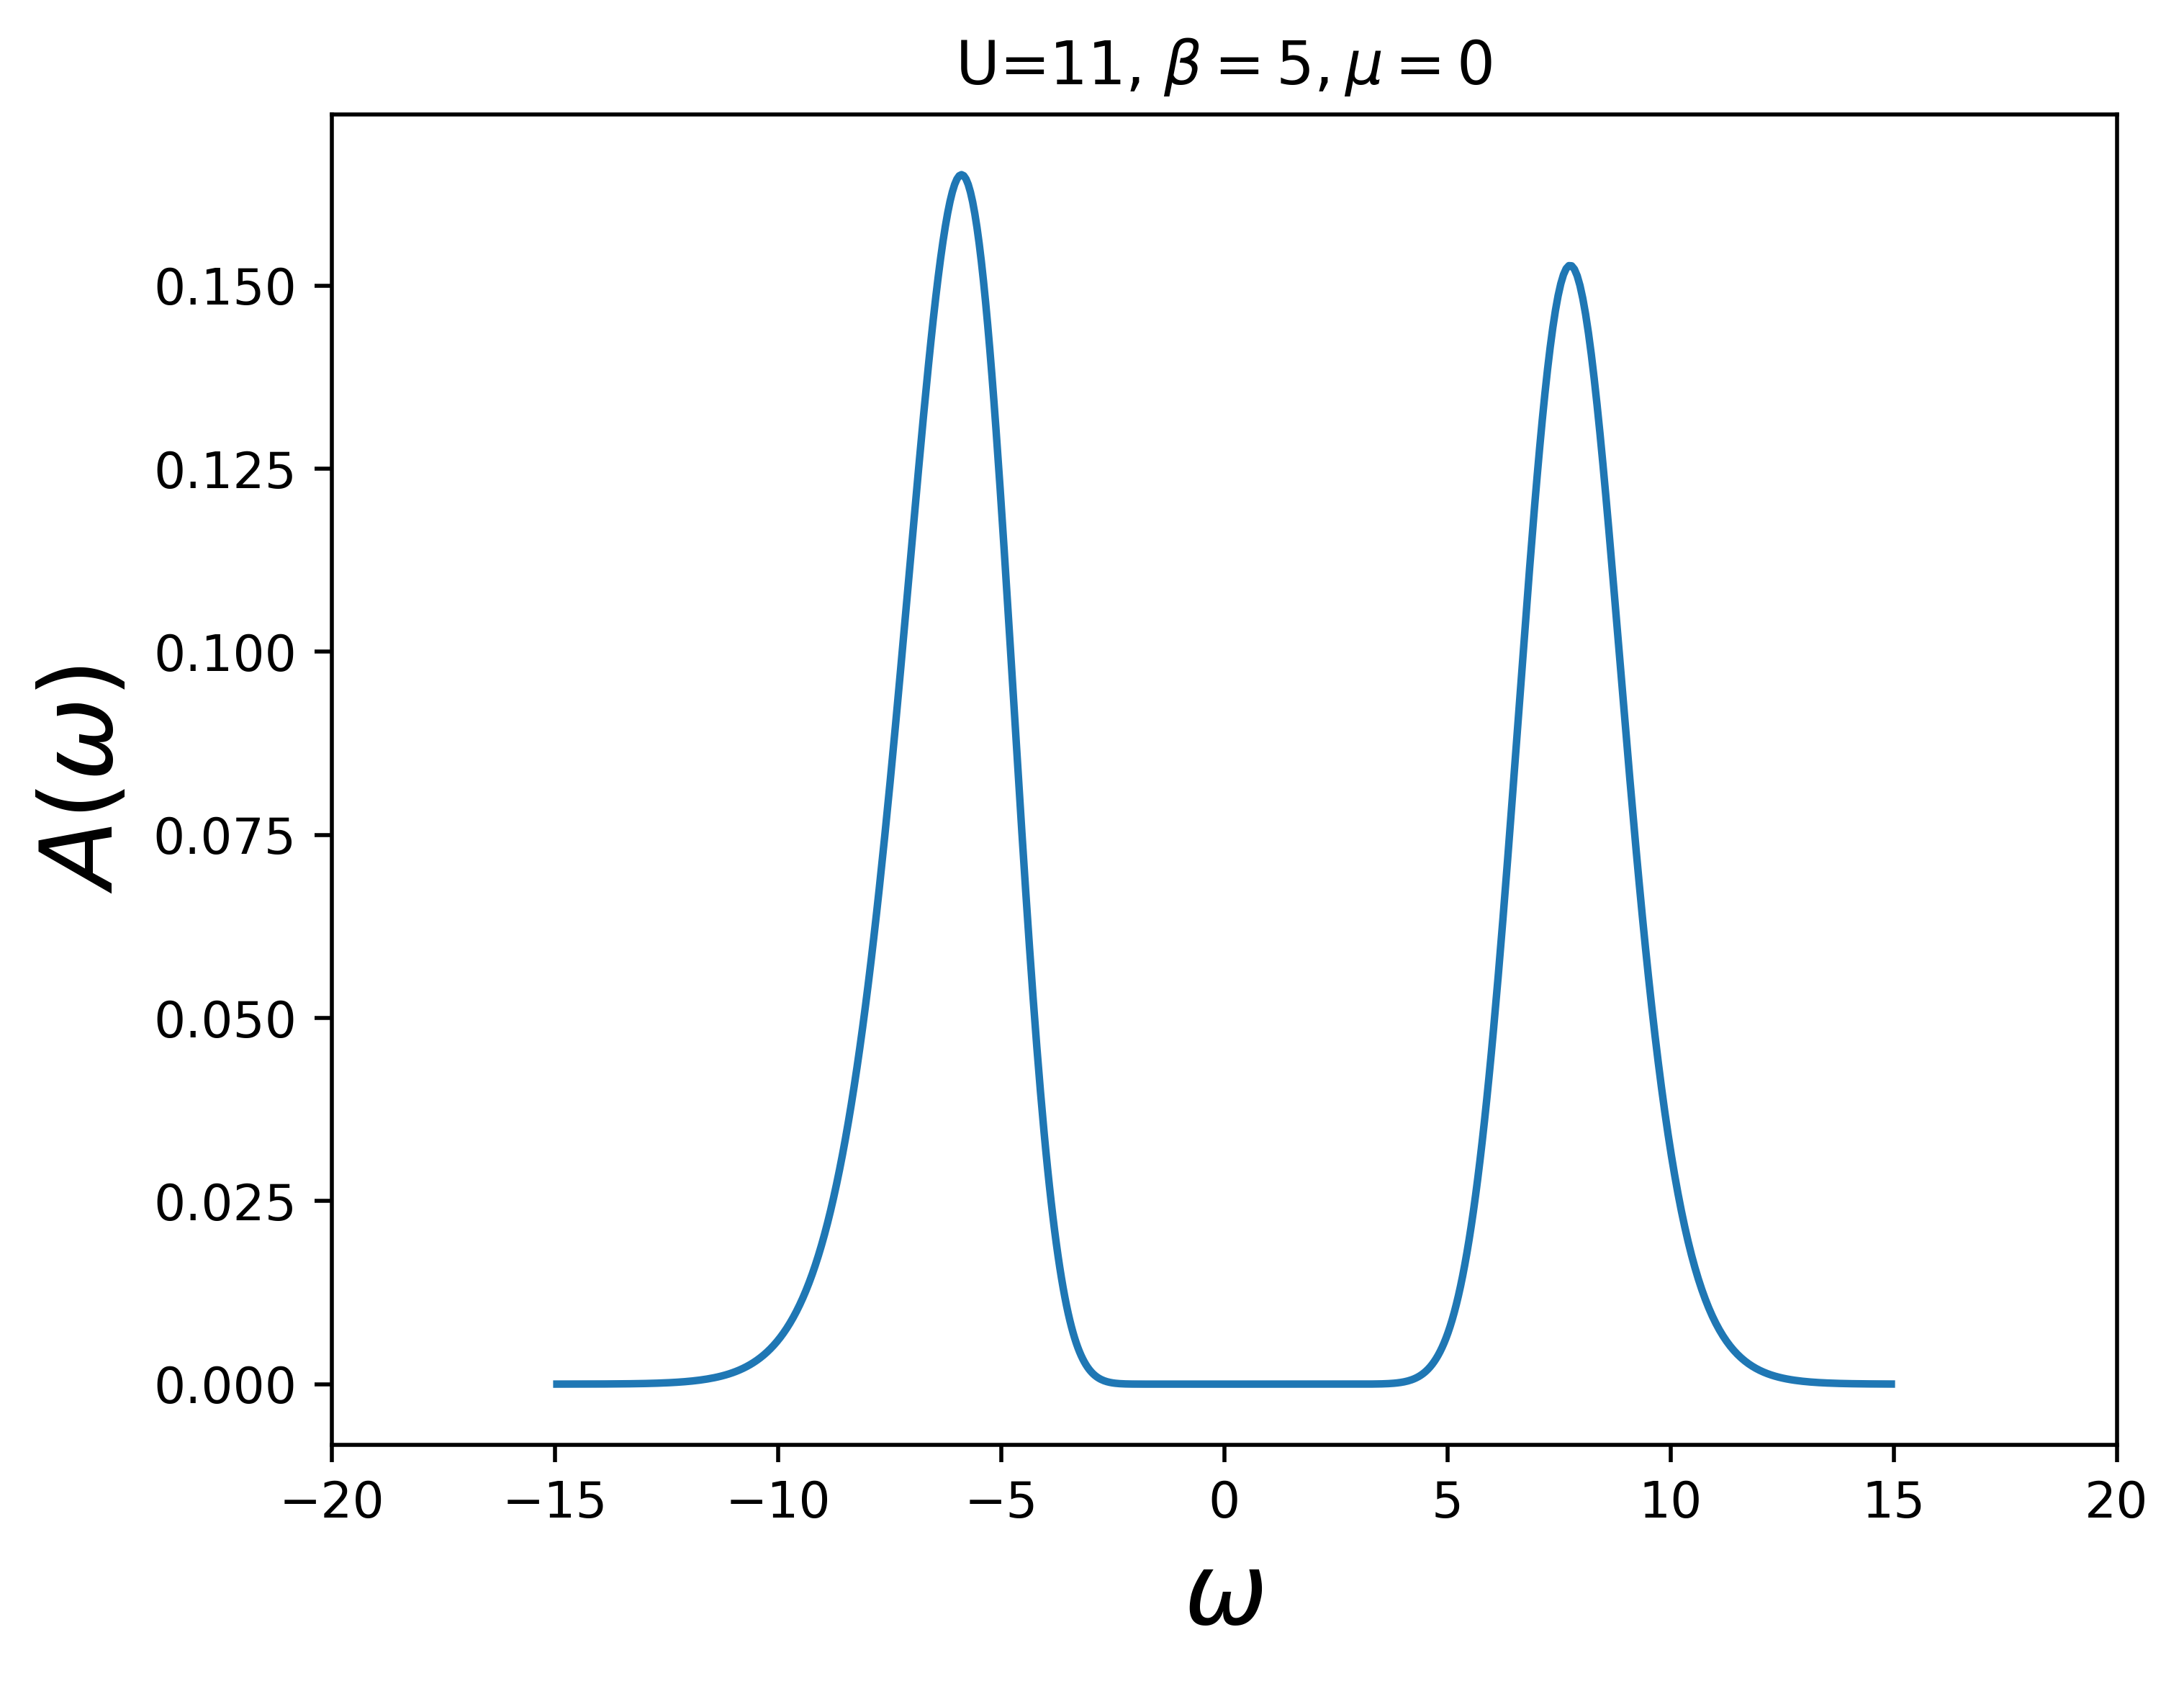
\includegraphics[width=0.45\linewidth]{fig2/dfspectral11.png}
    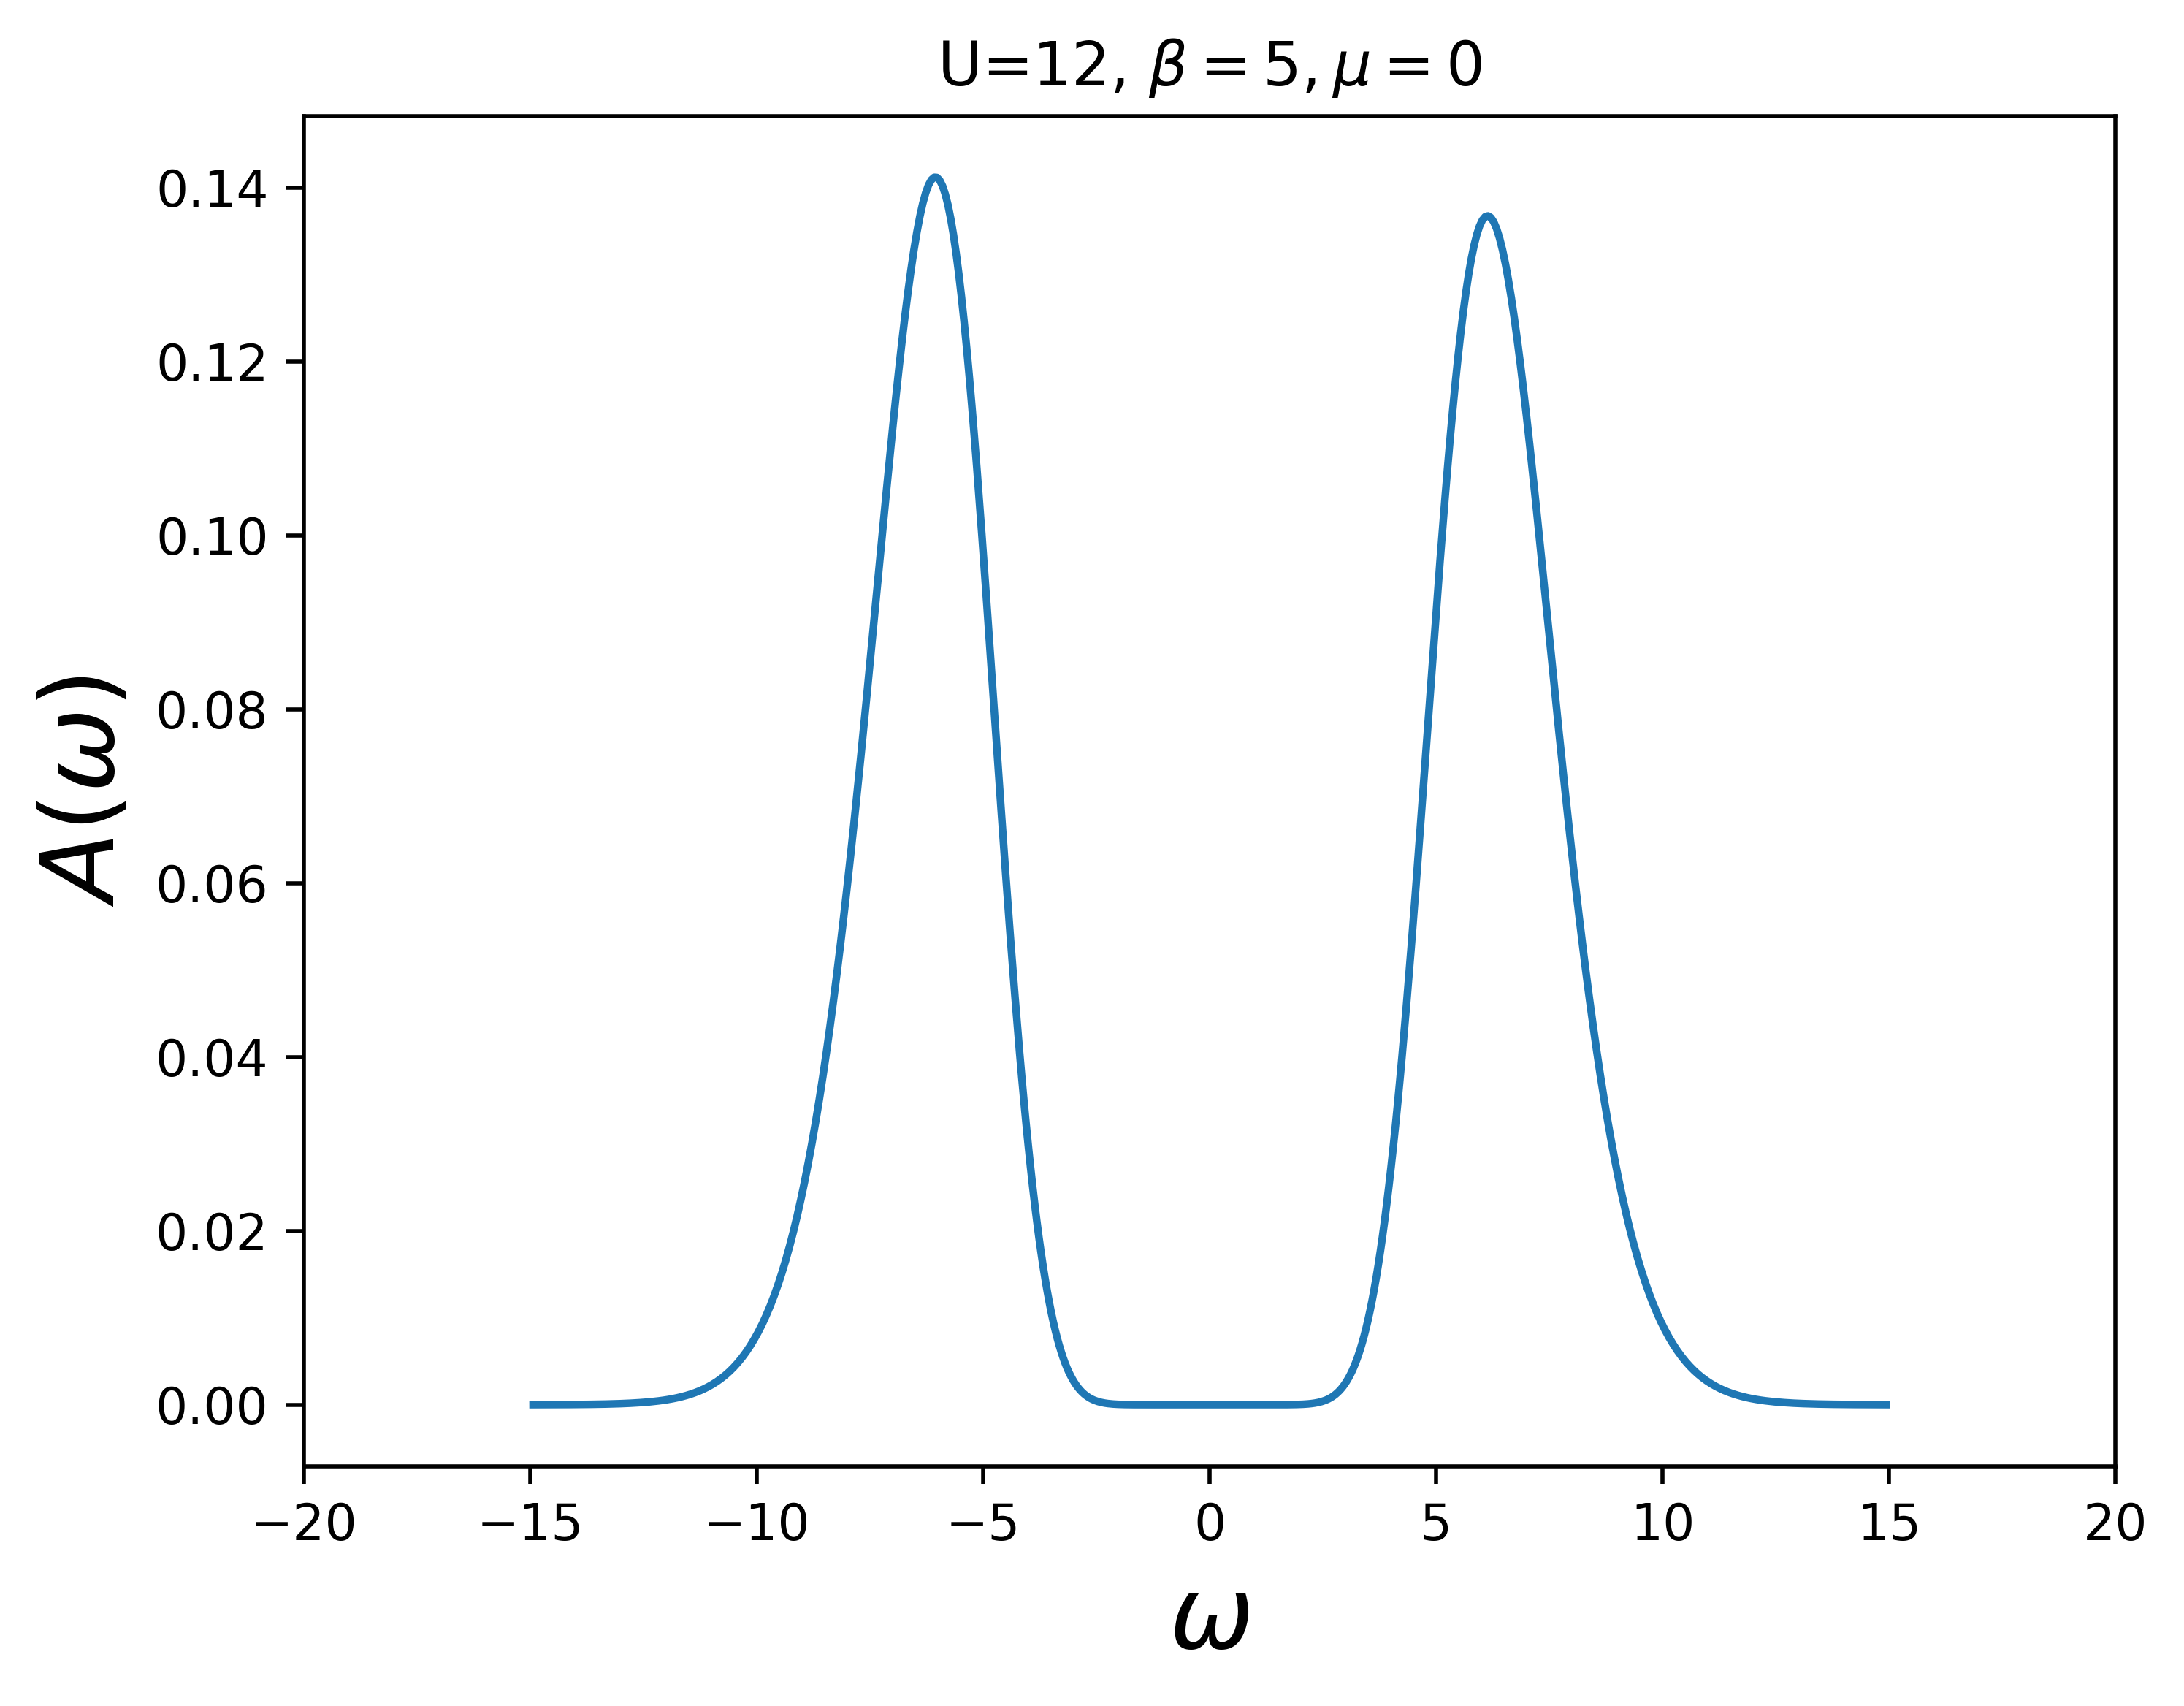
\includegraphics[width=0.45\linewidth]{fig2/dfspectral12.png}
    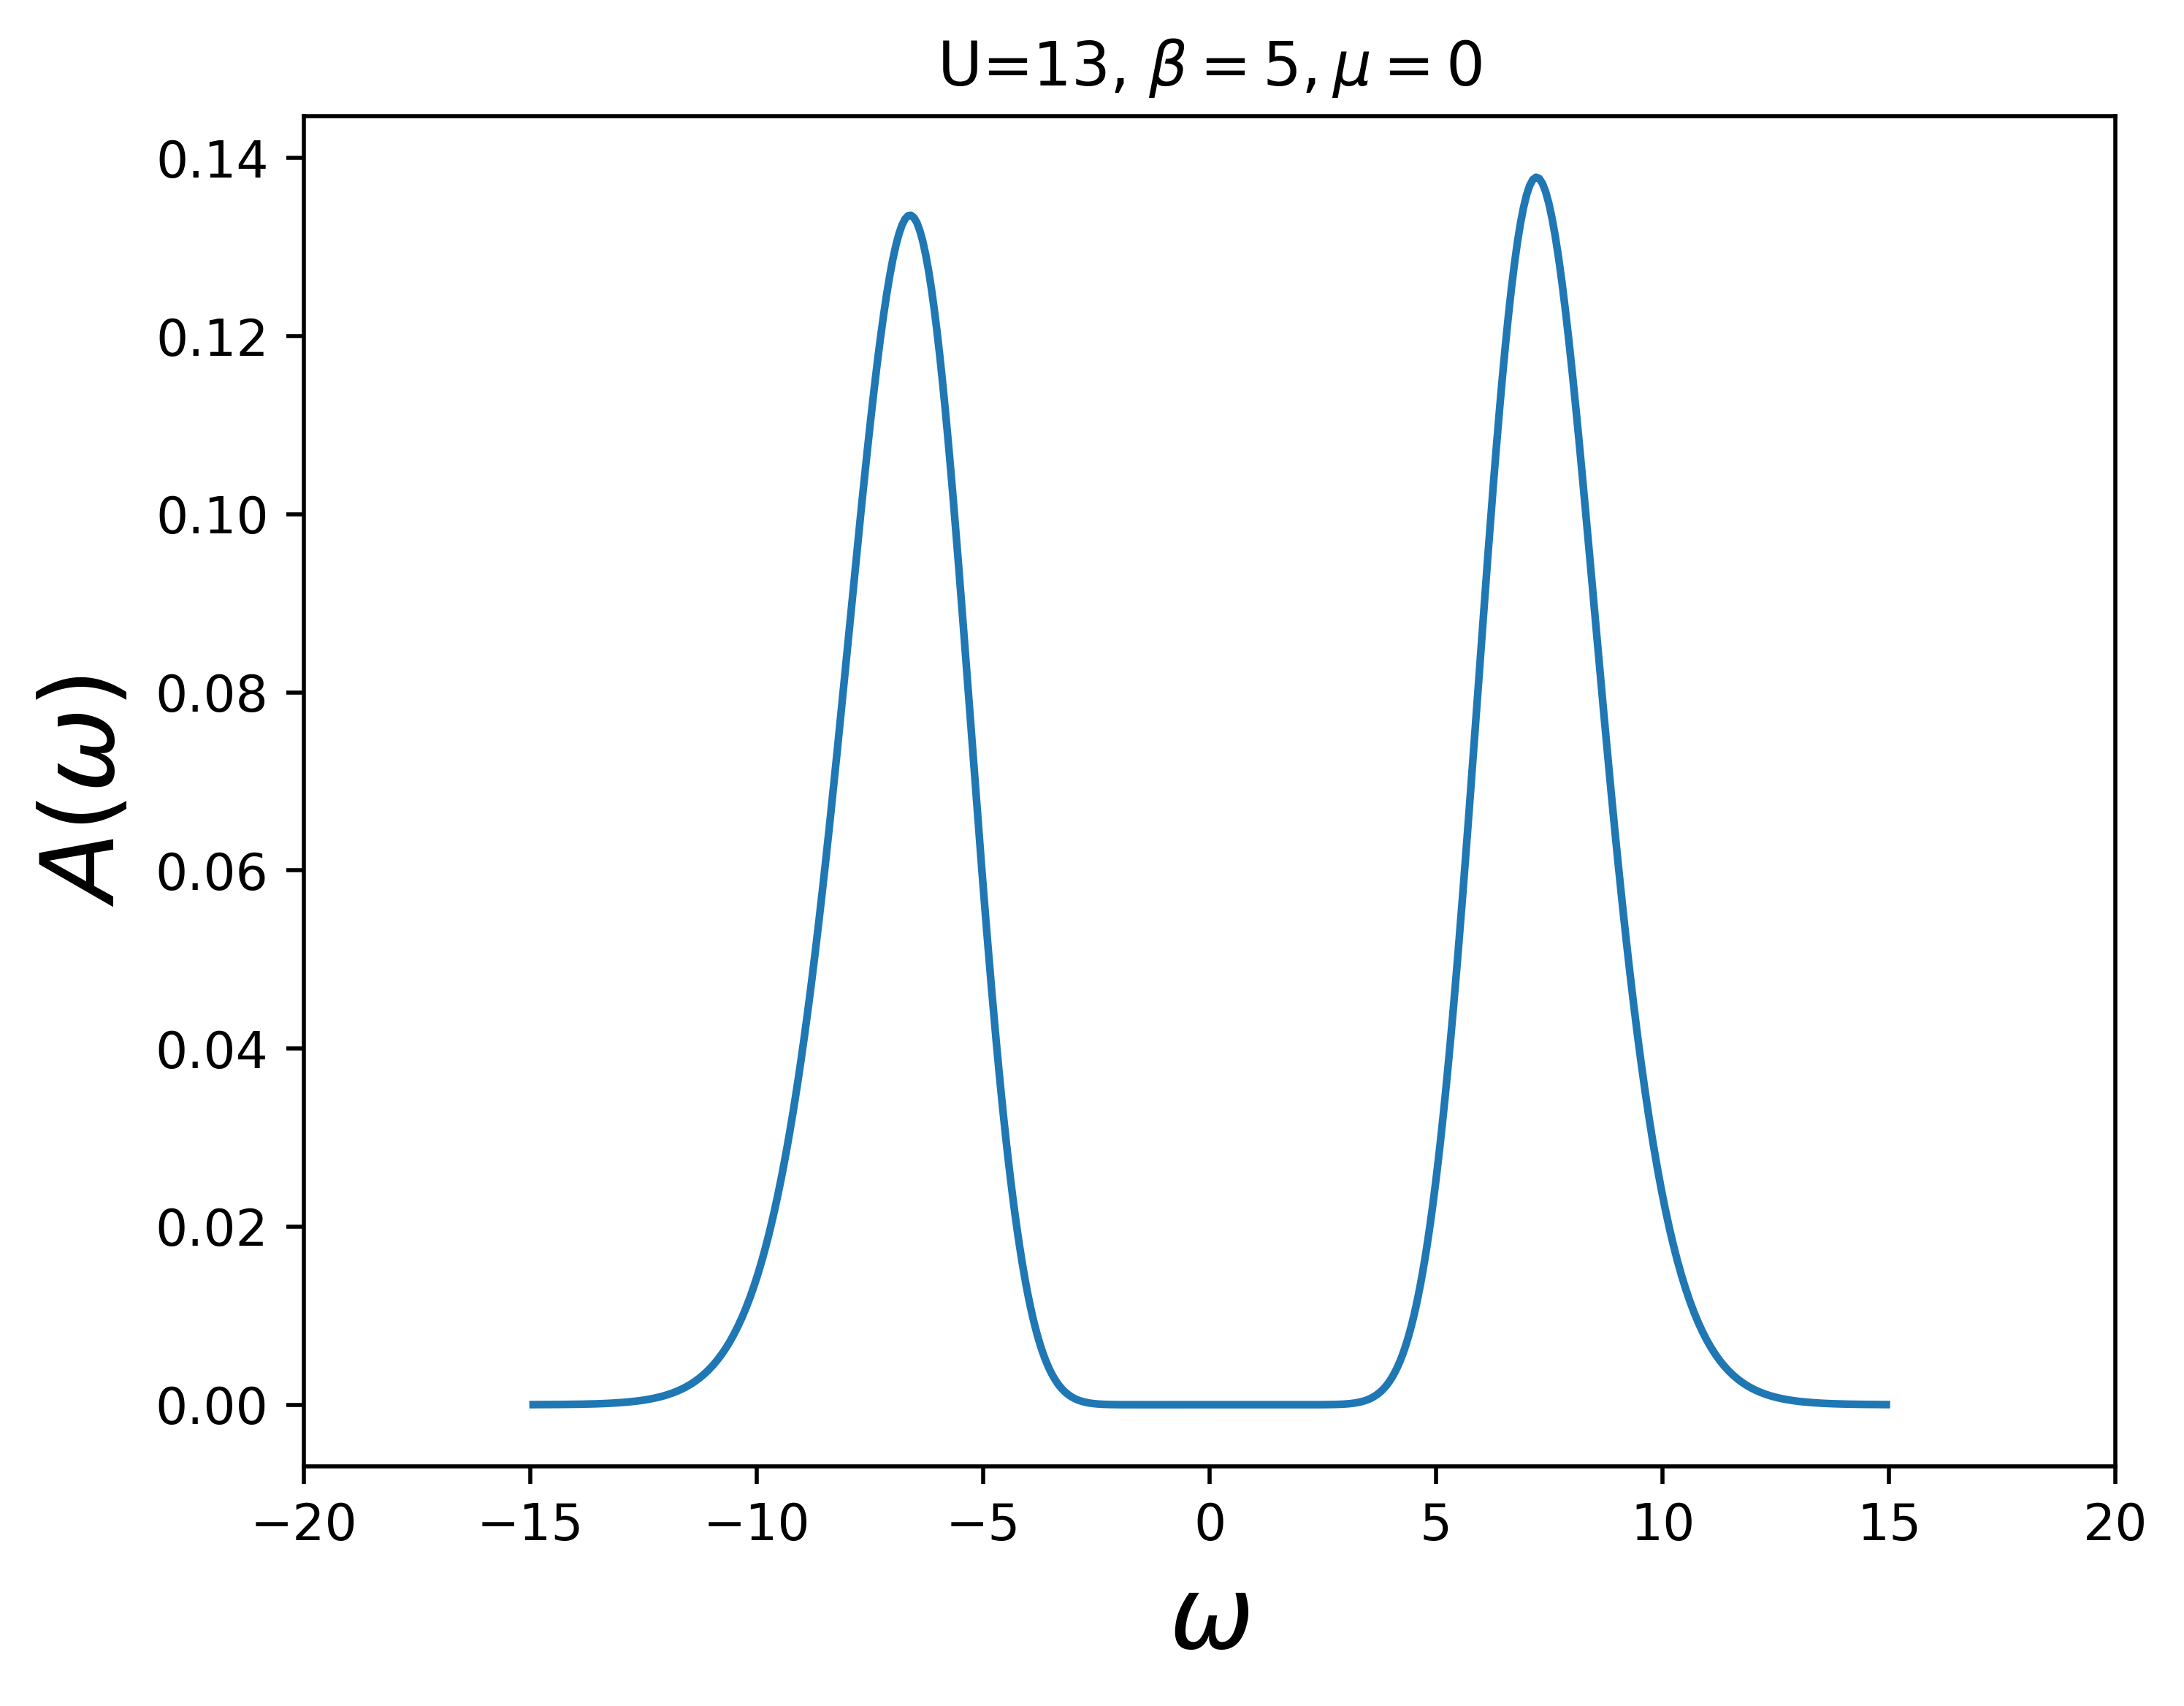
\includegraphics[width=0.45\linewidth]{fig2/dfspectral13.png}
    
\caption{ Spectral function, output of Maxent from Open- DF results for $U=3$ to $U=13$. Transition from Fermi liquis state to non-Fermi liquid state can be seen, gap appears between $U=5.6$ and $U=8$. \label{fig:DF_spectral}}
\vspace{-20pt}
\end{figure} 




\section{Dual Fermions (DF)}

\begin{figure}[ht]
\centering
    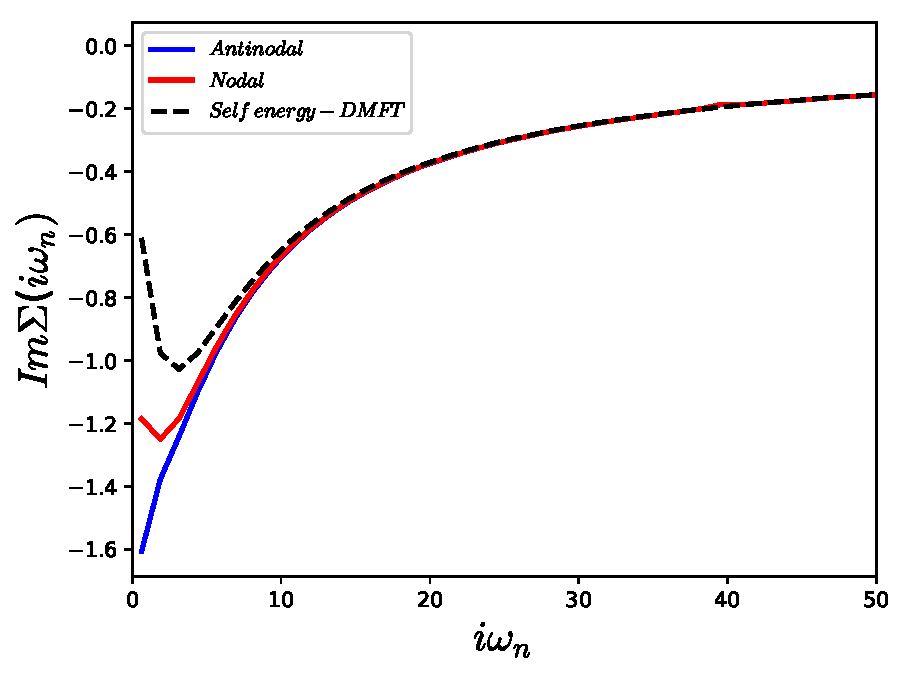
\includegraphics[width=0.9\linewidth]{fig3/selfenergy.pdf}
\caption {Imaginary part of the self energy as a function of Matsubara index for the DF Nodal (N) $(k= (\frac{\pi}{2},\: \frac{\pi}{2}))$ and Anti-nodal (AN) $(k= (0, \pi))$ results and the DMFT result. In this figure parameters for DF are  $U/t=5.6$, $\beta =5$, $t^\prime =-0.3$ and $\mu=0$.  Inset: Analytic continuation result for the spectral function, $A(\omega)$ for real frequency $\omega$.
\label{fig:Self_ Energy}}
\end{figure}

We access to DMFT self-energy $(\sum ^{DMFT} (i\omega _n))$ and Dual Fermion self-energy $(\sum ^ {DF} (i\omega _n, k))$. For DF self-energy since we inserted momentum in our results, we can study its result in more details. So we consider two specific points in the Brillouin zone, Nodal $(k= (\frac{\pi}{2},\: \frac{\pi}{2}))$ and Anti-Nodal points $(k= (0, \pi))$. By comparing the two first Matsubara frequencies $(\omega _n = \frac{(2n +1) \pi}{\beta})$, we can define the status of the system $(\Delta\Sigma=Im \sum (i\omega _0) - Im \sum (i\omega _1))$. If $Im \sum (i\omega _0) < Im \sum (i\omega _1)$ $(\Delta\Sigma<0)$ the system is an insulator, otherwise, if $Im \sum (i\omega _0) > Im \sum (i\omega _1)$ $(\Delta\Sigma>0)$ the system is in Fermi Liquid regime (metallic state) \cite{Geles, Wei}.

In Fig.~\ref{fig:Self_ Energy} we present DF results at $U/t=5.6$, $t^\prime=-0.3$, $\mu=0$, $\beta =5$ for the imaginary part of the self energy. The DMFT result (dashed-black) shows a tendency towards FL behaviour. It is clear that the first Matsubara frequency has a higher value than the second, so ($\Delta \Sigma > 0$).  Red and blue curves are results at the nodal and antinodal momenta respectively from the DF calculation which provides momentum dependence to the self-energy. 
We note for these parameters the shift from FL to partial nFL behaviour indicated by the negative value of $\Delta \Sigma$ at the antinodal point and this mean the system is an insulator, while the nodal point remains with $\Delta \Sigma >0$ and the system shows metal behaviour. This behavior is often referred to as the pseudogap phenomenon \cite{Valli, Rice}.
Our results are in a good agreement with  DiagMC and DCA calculations with similar parameters from  Ref. \cite{Wei}. 
 
\begin{figure}[ht]
\centering
    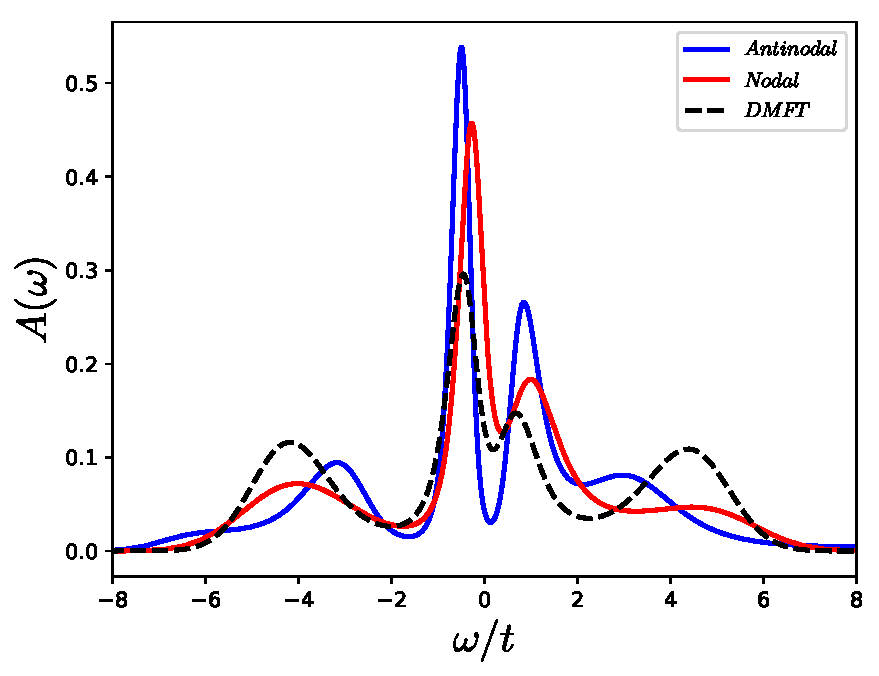
\includegraphics[width=0.9\linewidth]{fig3/spectral.pdf}
\caption {Analytic continuation result for the spectral function, $A(\omega)$ for real frequency $\omega$. In this figure parameters for DF are  $U/t=5.6$, $\beta =5$, $t^\prime =-0.3$ and $\mu=0$.
\label{fig:spectral_self}}
\end{figure}


Since these results for $\beta =5$ are at relatively high temperature, finding $\Delta \Sigma <0$ may not be a good index of a fully gapped state. Therefore, to show this, we found their spectral function by performing analytic continuation \cite{maxent} for the local-DMFT Green's function, and the Green's function for the DF nodal and antinodal results.  
The normalized spectral functions, $A_k(\omega)$, is shown in Fig. \ref{fig:spectral_self}. Indeed, what we have found is a non-zero density of states at the Fermi level ($\omega=0$) that is caused by thermal excitations. 
We do not observe a clear $\omega=0$ FL peak and the value of $A(\omega=0)$ for the antinodal point is $\approx 15\%$ of the nodal value an indication of the erosion of states at the Fermi level. 


\begin{figure}[ht]
\centering
    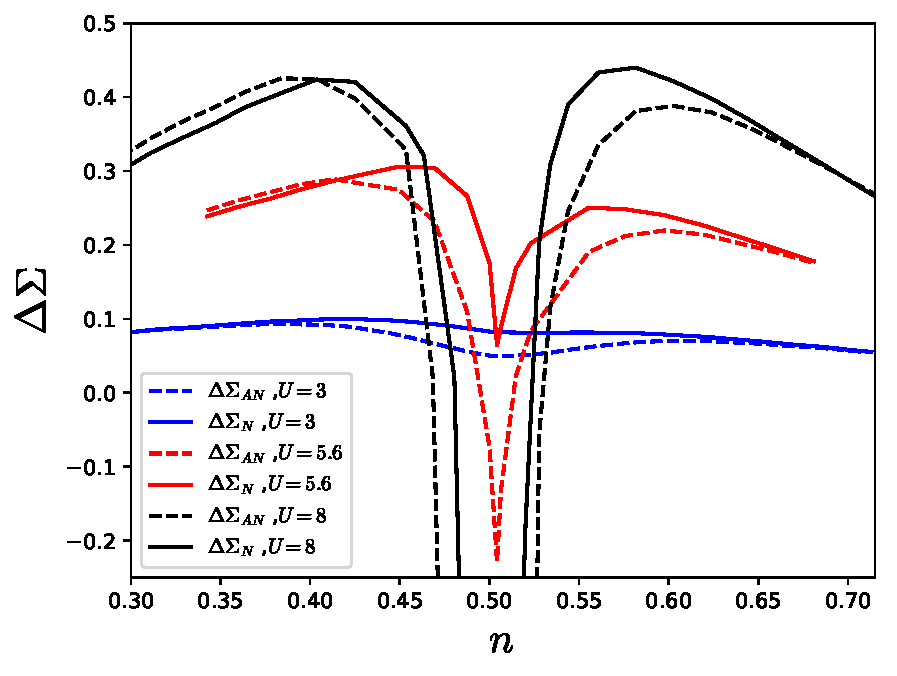
\includegraphics[width=0.8\linewidth]{fig3/deltasigma_all.pdf}
\caption{ $\Delta \Sigma$ at the nodal ($\Delta \Sigma_{N}$) and antinodal ($\Delta \Sigma_{AN}$)  momenta as a function of density for various $U/t$ at $\beta t=5$ and $t^\prime /t=-0.3$. 
\label{fig:deltasigma_all}}
\end{figure} 

Next, we investigate the variation of $U/t$ and density, $ n $, on $\Delta \Sigma$ at fixed temperature. By studying the $\Delta \Sigma$ we can reveal the behaviour of the material in different densities and show how a change in the density can change our system from FL to nFL (metallic to insulator) or vice verse. 

We depict our results in Fig.~\ref{fig:deltasigma_all} where we plot the value of $\Delta \Sigma$ at the nodal and antinodal points.  At this relatively high temperature we see that at $U/t=3$, $\Delta \Sigma$ is positive for all densities ,which represent FL states at all momenta. 
At $U/t=5.6$ we see a region of density near half-filling where $\Delta \Sigma_{AN}<0$ while $\Delta\Sigma_N$ is always positive that show a mixed FL/nFL momentum separation near half-filling.   For $U/t=8$, both the nodal and antinodal points show nFL behaviour (insulator) over a range of densities (wider for the AN point) becoming positive with either electron or hole doping away from half-filling $(\mu = 0)$ \cite{Gull10,gull:2009}.
Our results at high temperature of a crossover with interaction strength are in agreement with the cDMFT phase diagram and shows transition from FL to nFL region \cite{park}. What is unclear is the physical origin of the nFL behaviour, if it is a first order Mott transition or is caused by AF spin fluctuations.

\begin{figure}[ht]
\centering
    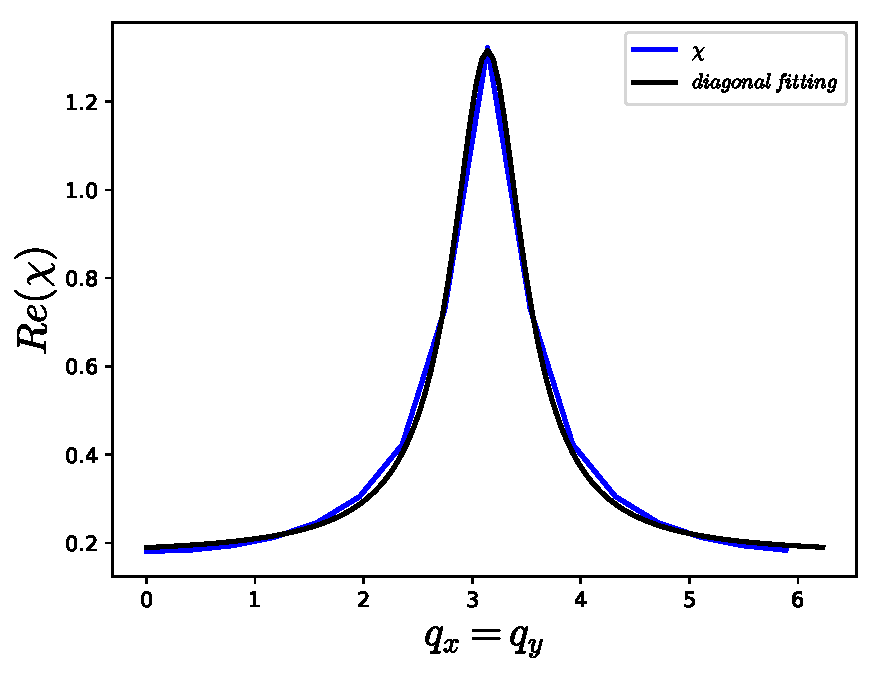
\includegraphics[width=0.6\linewidth]{fig3/fit.pdf}
    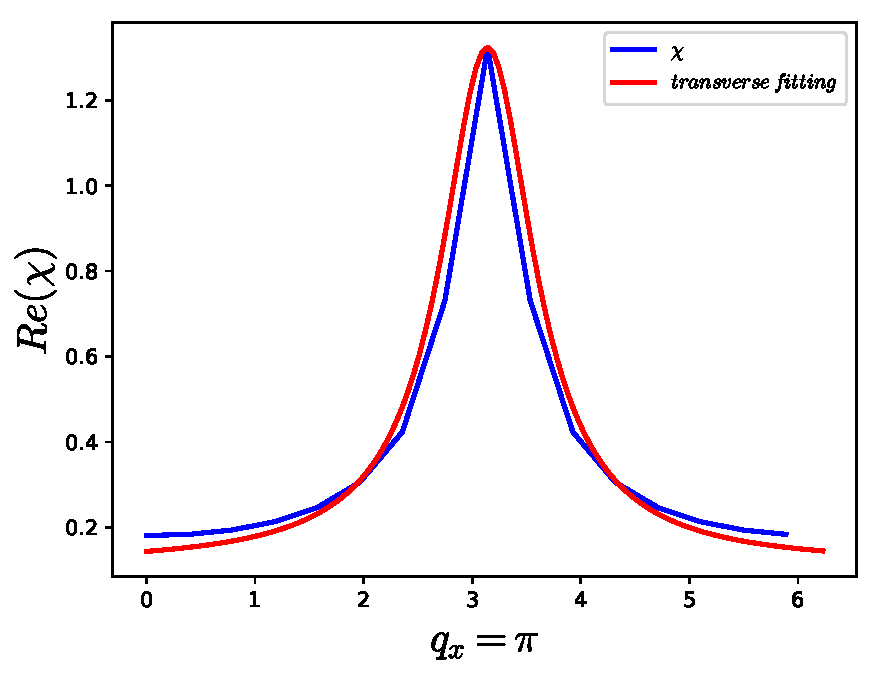
\includegraphics[width=0.6\linewidth]{fig3/fit1.pdf}
%    \includegraphics[width=0.3\linewidth]{cor_U}
        \caption{\label{fig:fit}Curve fitting obtained from a fit of $\chi_{sp}(q_x,q_y,\Omega=0)$ with the function $f(q_x,\xi)=A/((\mathbf{q}-(\pi,\pi))^2+\xi^{-2}) +c $, averaged over the $q_x=q_y$ and $(q_x,q_y)=(q_x,\pi)$ directions, parameters are $U=3$, $\beta=5$ and $\mu=0$.\cite{rohringer:2016, gukelberger:2017}}
\end{figure}


Another output of the Dual Fermion calculations is susceptibility, $\chi_{sp}(q_x,q_y)$. $\chi_{sp}$ can be used to extract the correlation length for the system. 
To do this we consider the two-particle spin susceptibility\cite{hafermann:2008,chen:2017} from which we extract the correlation length. To find the correlation length we perform a curve fitting and the correlation length would be the half-width at half-max of $\chi_{sp}(q_x,q_y,i\Omega=0)$ near $(q_x,q_y)=(\pi,\pi)$ which can be found by fitting data to the:

\begin{equation}
    f(q_x,\xi)=A/((\mathbf{q}-(\pi,\pi))^2+\xi^{-2}) +c .
\end{equation}

\noindent We find the half-width at half-max for two different directions $q_x=q_y$ and $(q_x,q_y)=(q_x,\pi)$ then the average of these two direction would be the correlation length Fig.~\ref{fig:fit} shows this process. 


\begin{figure}[ht]
\centering
    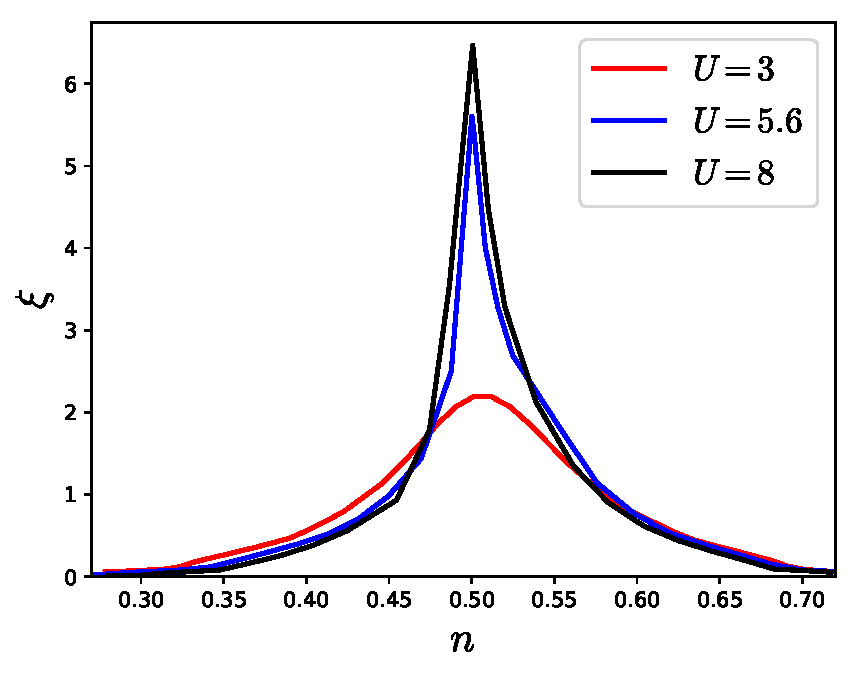
\includegraphics[width=0.8\linewidth]{fig3/density_cor.pdf}
%    \includegraphics[width=0.3\linewidth]{cor_U}
        \caption{\label{fig:corlengthdoping}Density dependence of the anti-ferromagnetic correlation length, $\xi$, for several interaction strengths $U$ at $T/t=0.2$. Obtained from curve fitting.\cite{rohringer:2016, gukelberger:2017}}
\end{figure}

 In Fig.~\ref{fig:corlengthdoping} we depict our results for correlation length $(\xi)$ as a function of density for different energies.  If we make a comparison between Fig.~\ref{fig:deltasigma_all} and Fig.~\ref{fig:corlengthdoping} we see that there is a connection between the nFL and FL behavior in the self energy as a function of density (doping) to the increase in spin-correlation length, $\xi$.  
At this high temperature for $U/t=3$ the value of $\xi \lesssim 2$ lattice sites is quite small and comparing with Fig.~\ref{fig:deltasigma_all} we see that $\Delta \Sigma$ is positive for all densities.  At $U/t=5.6$ and 8, $\xi$ has a much larger value for a range of dopings near $n=1$.  It seems that the increase of $\xi$ with doping coincides with a reduction of $\Delta \Sigma$ ultimately resulting in a change of sign.  Interestingly, at these high temperatures with modest $t^\prime$, the value of $\Delta \Sigma$ is not substantially distinct between hole or electron doping ($n<1$ and $n>1$ respectively).  The antinodal point shows a tendency towards nFL behaviour for both electron and hole doped cases. This might be because of the tendency towards antiferromagnetic behaviour that is driving the FL/nFL crossover.

\section{Fluctuation Diagnostics}

The self-energy explains all scattering effects while an electron propagates through the lattice. In correlated electronic systems, these scattering events come from the Coulomb interaction among the electrons themselves. The single particle self-energy can be determined from the full two-particle vertex function in the spin basis $F_{sp}$,\cite{Valli, Toschi} and also by  interacting lattice Green's function $g(k,\omega)$ ,which is a function of both momentum and frequency, via:

\begin{equation}
    \Sigma(k,\omega)= \frac{Un}{2}+ \frac{U}{\beta^2 N} \sum \limits_{\bar{\omega}^\prime ,\bar{\Omega}} F_{sp}^{\bar{\omega},\bar{\omega}^\prime,\bar{\Omega}} g(\bar{\omega}^\prime)g(\bar{\omega}^\prime +\bar{\Omega}) g(\bar{\omega}+\bar{\Omega})
    \label{eqn:fluct}
\end{equation}

\noindent Where $U$ is the Hubbard interaction, $n$ is the density, $\beta = \frac{1}{T}$ is the
inverse temperature, $N$ is the normalization of the
momentum summation, $g$ is the electron Green's function and $\bar{\omega}=(k,\omega)$, $\bar{\omega}^\prime=(k^\prime,\omega^\prime)$, $\bar{\Omega}=(q,\Omega)$, which $\omega$ and $\omega^\prime$ are fermionic frequencies and $\Omega$ represents a bosonic Matsubara frequency. Choosing the basis for the full vertex has no impact on the self-energy after summation over all internal indices of the vertex \cite{Toschi}.

In this thesis, we just study the spin channel, because former literature has suggested that for the single band model the charge and particle-particle channels are less structured, so we confined ourselves to the spin channel. Also we neglect the Hartree shift. We will study the complete set of Fermionic and Bosonic Matsubara frequencies and momentum space. To perform this we propose a partial summations given by:

\begin{equation}
    \Sigma_k^{(x)}= \sum\limits_{x, \bar{\omega}^\prime} \Sigma(\bar{\omega},\bar{\omega}^\prime, \bar{\Omega}).
\end{equation}

This summation is over: positive and negative scattering momenta, $x=q$, or all bosonic frequencies, $x= +\Omega, -\Omega$  or $\Omega$ respectively; or it can be over combinations of variables such as $x=(+\Omega, q)$ which means it is a summation over positive bosonic frequencies and all q-vectors. Also, we always sum over all the internal primed fermionic elements $\bar{\omega}^\prime$. We do this to reduce the dimensionality of our system which is convenient since $\bar{\omega}^\prime$ does not appear in our notation, neither in either single particle self energies nor two particle susceptibilities.

In Dual Fermion method to solve two particle Green's function and vertex of the impurity problem we choose a period of fermionic and bosonic frequencies, $\Omega= -32 \to 32= \Omega_c$ and $\omega,\omega^\prime = -64 \to 63=\omega_c$ inclusive. The self-energy is:

    \begin{equation}
     \Sigma(k,\omega)= \sum\limits_{ \bar{\omega}^\prime =-\omega _c}^{ \bar{\omega}^\prime =\omega _c}\sum\limits_{ \bar{\Omega} =-\Omega _c}^{\bar{\Omega} =\Omega _c} \Sigma(\bar{\omega},\bar{\omega}^\prime, \bar{\Omega}).
\end{equation}


\begin{figure}[ht]
\centering
    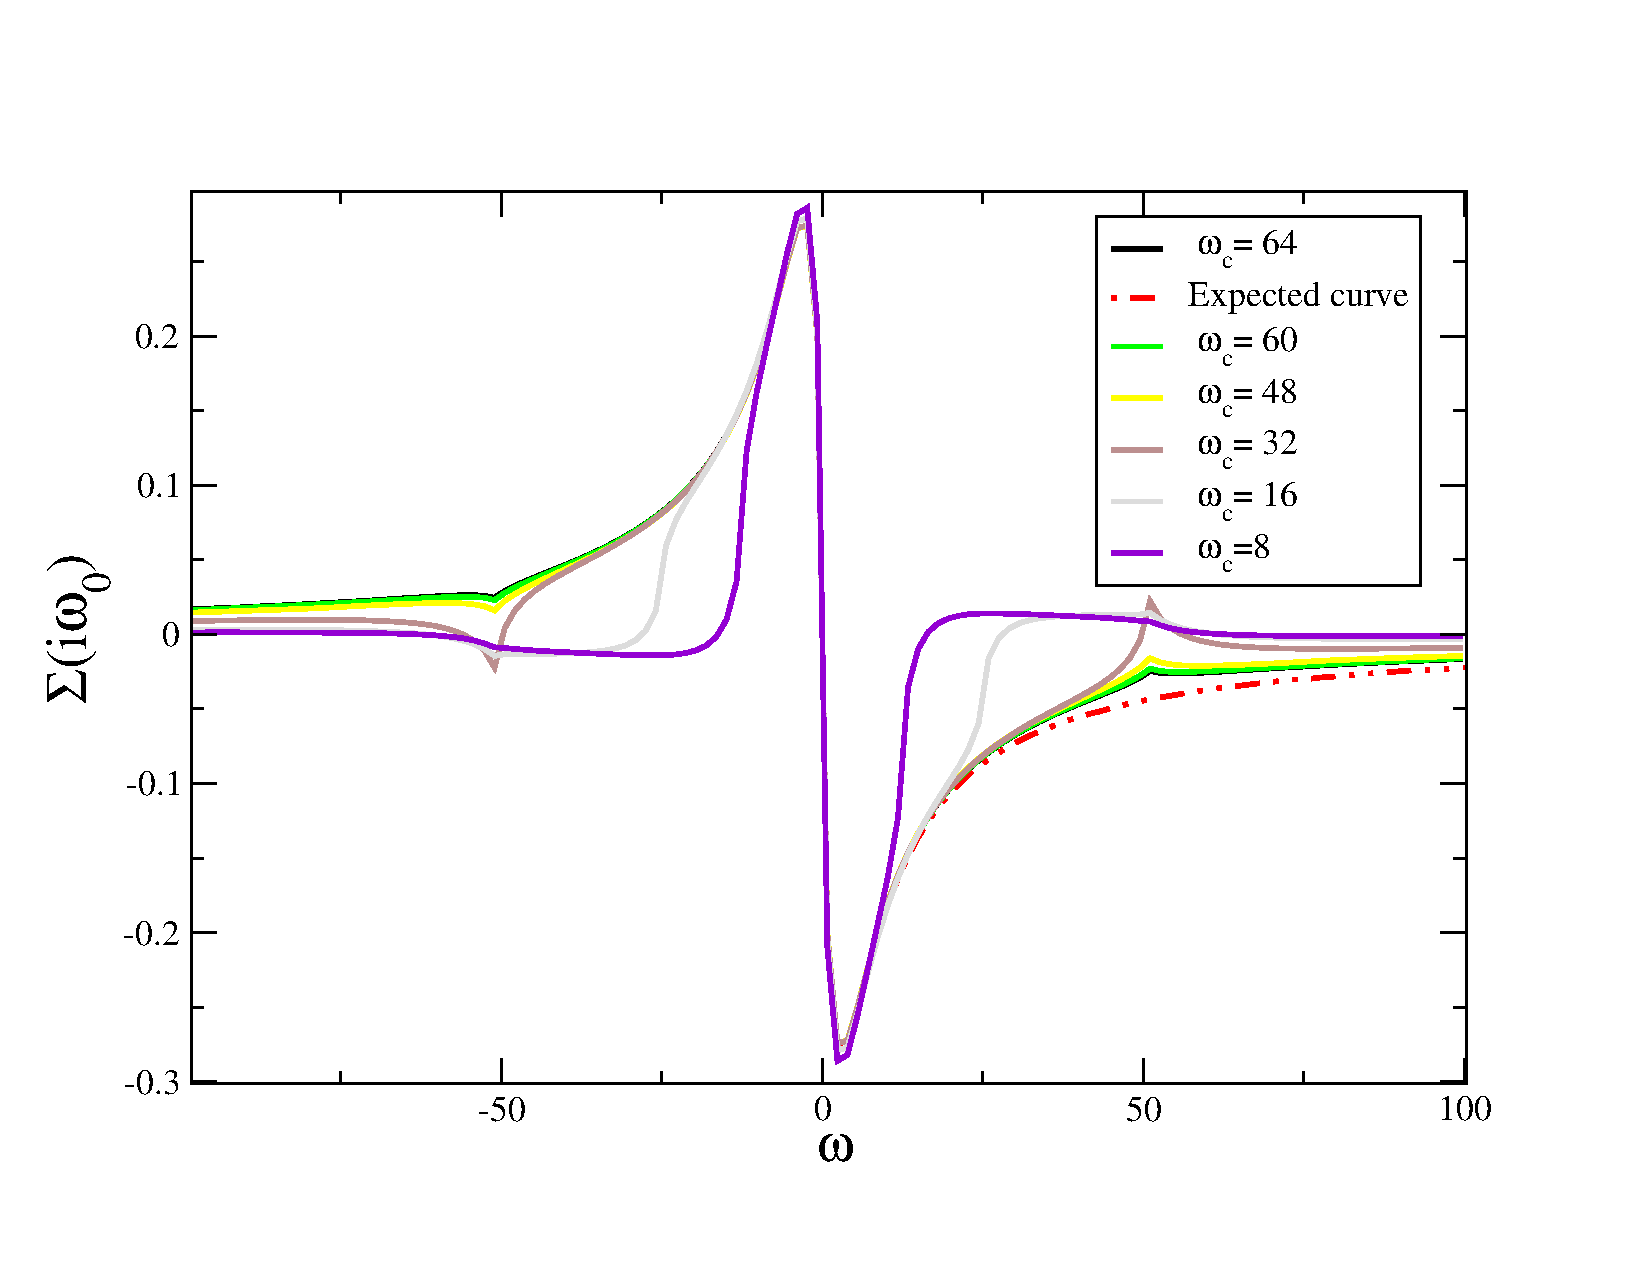
\includegraphics[width=0.50\linewidth]{fig2/self_energy_vs_nu.pdf}
    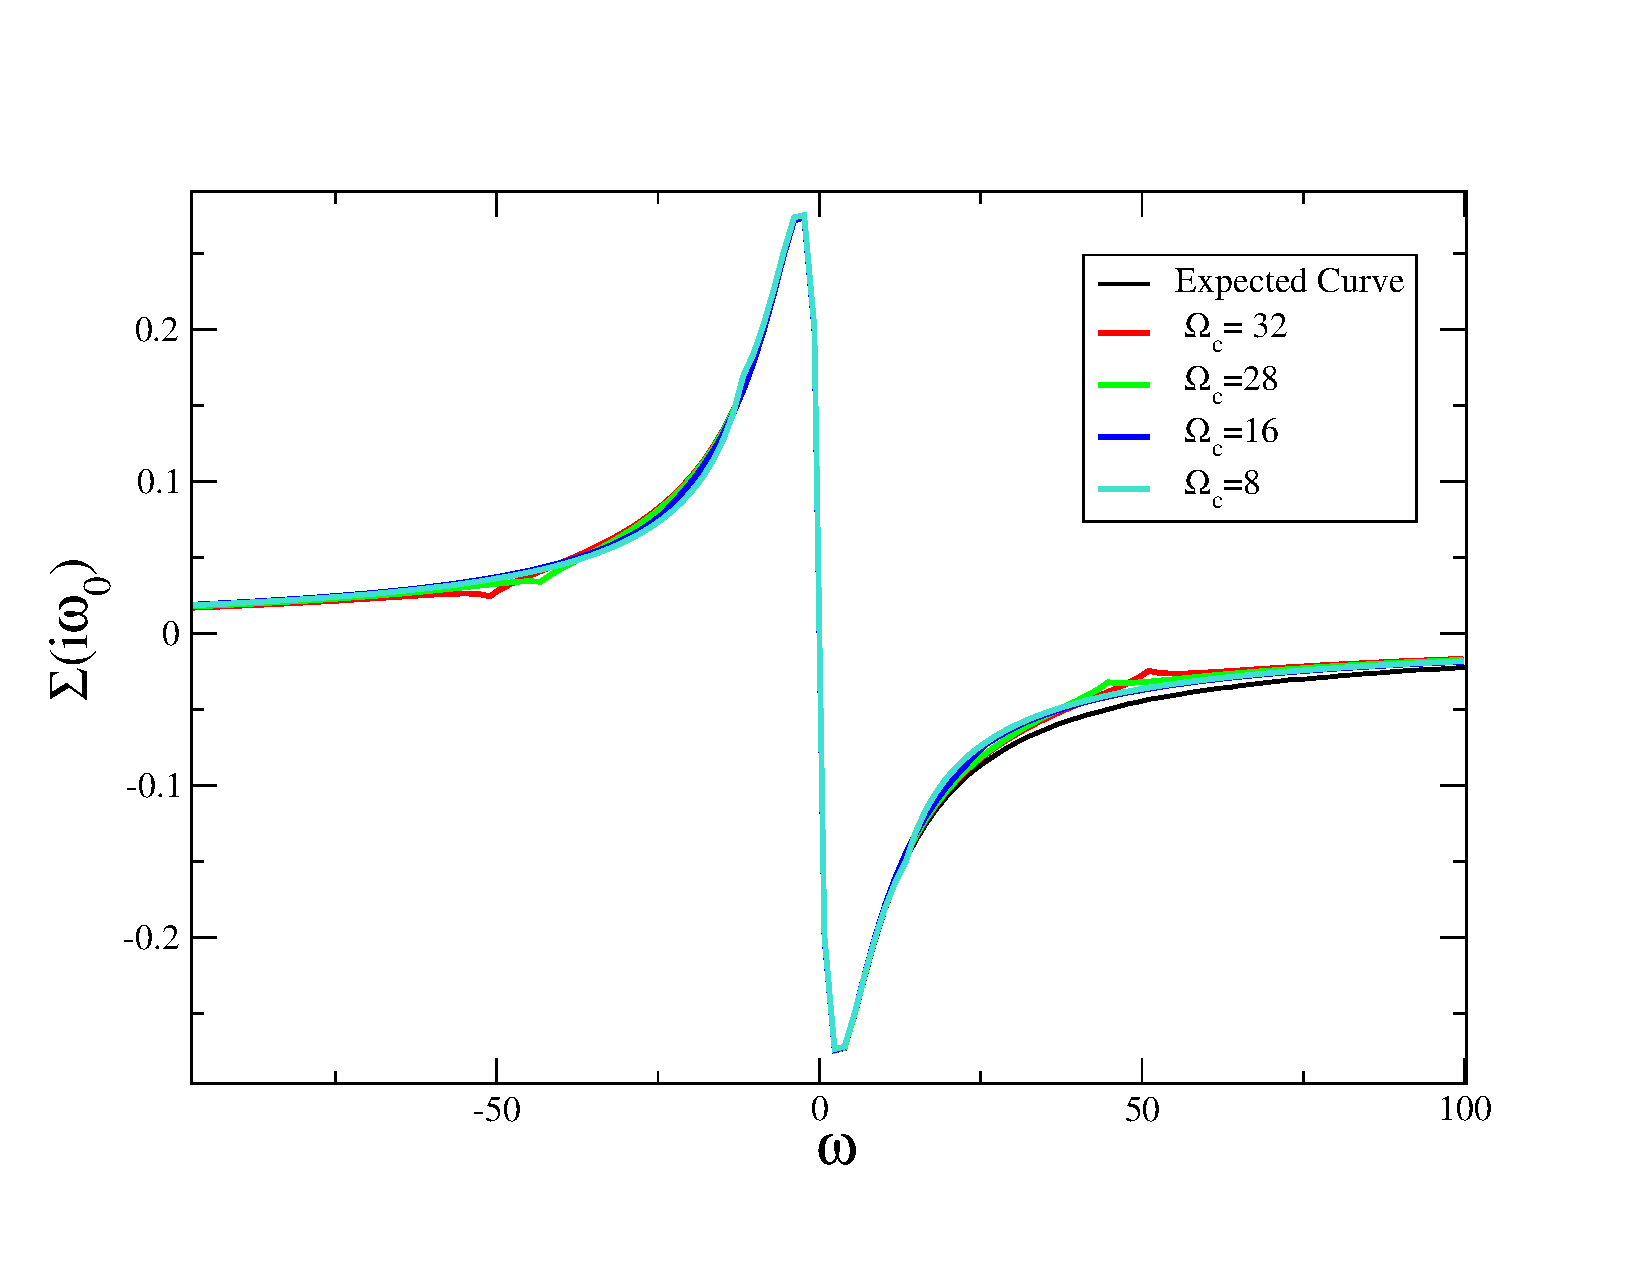
\includegraphics[width=0.50\linewidth]{fig2/self_energy_omega.pdf}
\caption{We show the effect of different cut off frequency on the self-energy. The left column represents the effect of Fermionic frequencies, and the right column depicts the effect of Bosonic frequencies on the self-energy. These plots prove that we have chosen the right period of Fermionic and Bosonic frequencies.
\label{fig:cutoff}}
\end{figure}

Fig.\ref{fig:cutoff}  displays the effect of different cut off frequency on the self-energy, it proves that we have chosen the right period of Fermionic and Bosonic frequencies to remake the self-energy. The left column represents the effect of Fermionic frequencies, and the right column depicts the effect of Bosonic frequencies on the self-energy. By increasing the value of frequencies, we increase the accuracy of our solution. 
These plots verify that our frequency set is large enough to accurately reconstruct the DMFT and DF self energies via Eq.~\eqref{eqn:fluct}.

Since we can decompose the single particle $\Delta\Sigma$ into the scattering momenta $(q_x , q_y)$ and frequency channels, we have access to different information that we are going to discuss in the following. 

\subsection{Self-energy}

\begin{figure}[ht]
\centering
    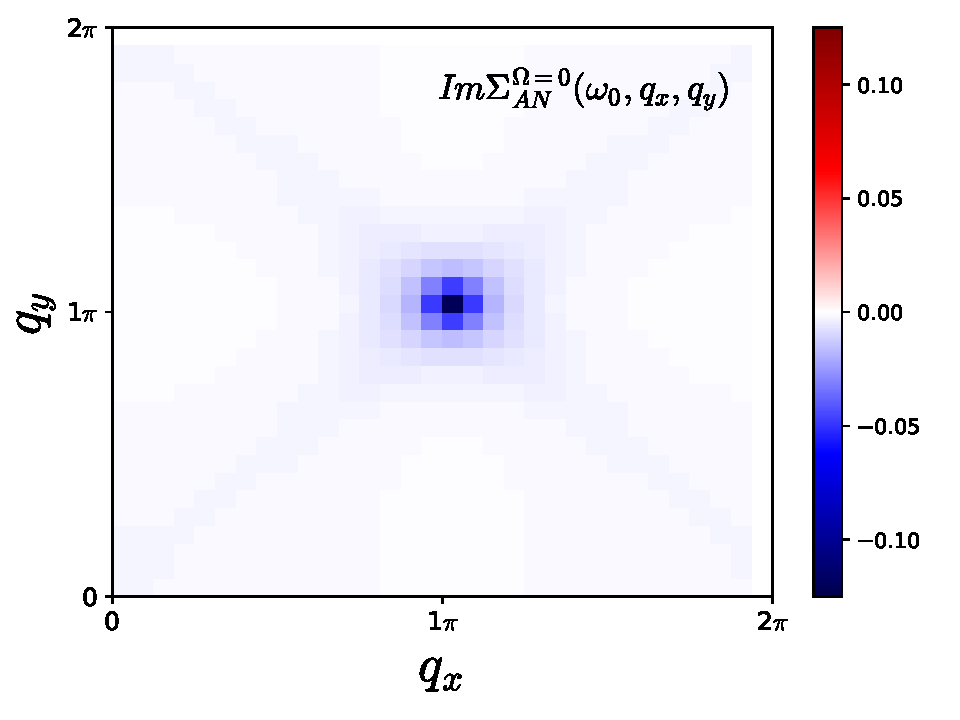
\includegraphics[width=0.48\linewidth]{fig3/c_mu_0_sigma_AN_nu1.pdf}
    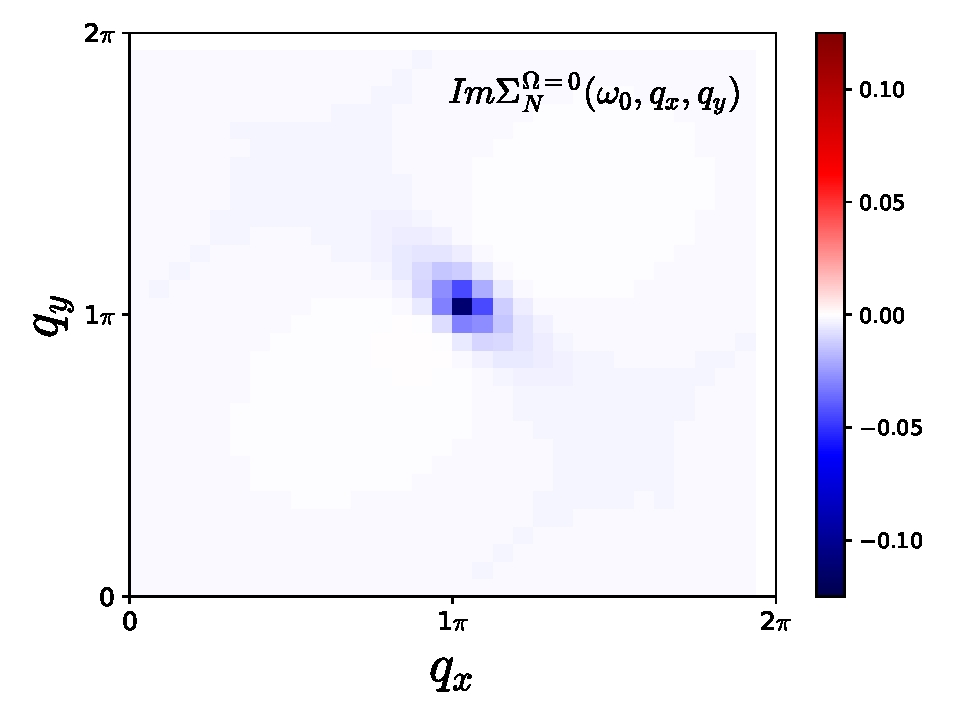
\includegraphics[width=0.48\linewidth]{fig3/c_mu_0_sigma_node_nu1.pdf}\\
    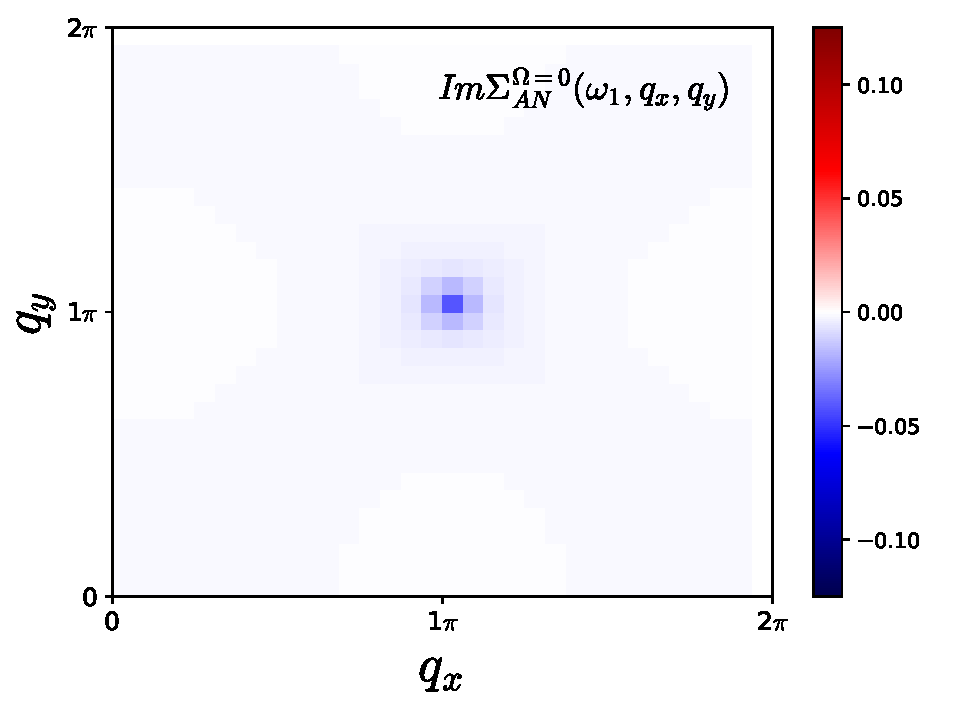
\includegraphics[width=0.48\linewidth]{fig3/c_mu_0_sigma_AN_nu2.pdf}
    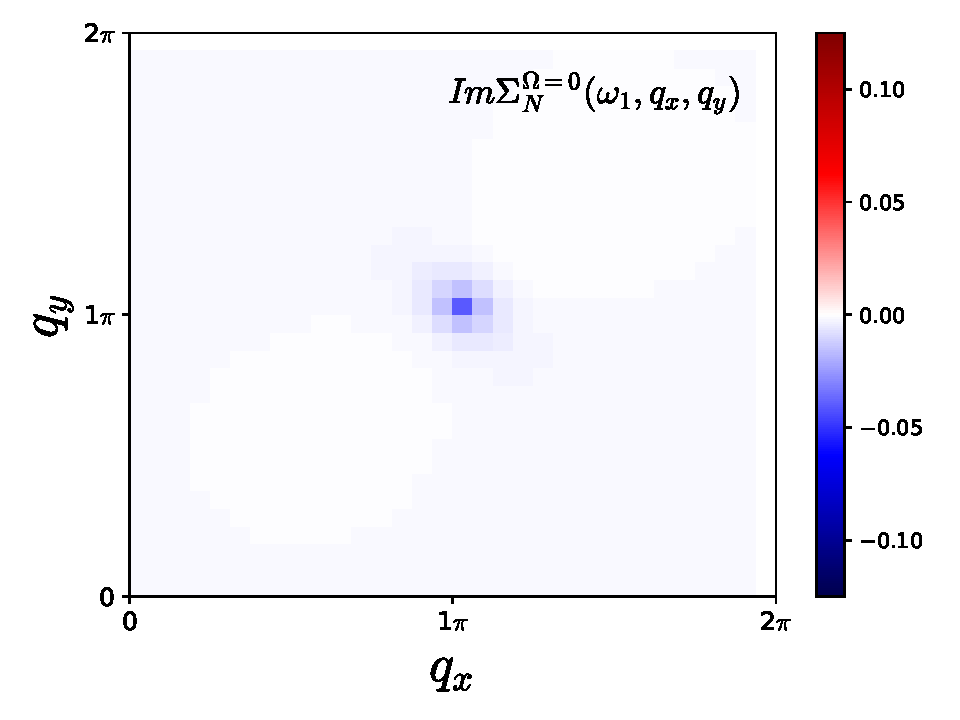
\includegraphics[width=0.48\linewidth]{fig3/c_mu_0_sigma_node_nu2.pdf}
    
\caption{  Imaginary part of the self energy for the antinodal (Left) and nodal (Right) momenta decomposed into the scattering $q=(q_x,q_y)$ contributions for the zeroth bosonic Matsubara frequency and first two Fermionic freq for $U/t=5.6$, $\beta t =5$, $t^\prime /t=-0.3$, and $\mu=0$.
\label{fig:sigma}}
\end{figure}

We start with self-energy, since we access to all frequencies and momentum. We represent the $q-$vector deconstruction of self-energy in Fig.~\ref{fig:sigma}. In this figure we show the fully deconstructed self-energy contributions to the zeroeth and first fermionic Matsubara frequency $i\omega_0 , i\omega_1$  at $\Omega=0$ as a function of the $q-$vector components. We use these two frequencies since we need to find $\Delta \Sigma$ by these two frequencies. Results of Refs \cite{Toschi, Wei} confirm what we have found. In Fig. \ref{fig:sigma} we see a strong peak at $q=(\pi,\pi)$ for both the N and AN $k-$vectors, and weaker contributions at other $q-$vectors. It's clear that basically all $q$-vector contributions to the self-energy are negative, consistent with other literature \cite{Toschi, chen:2017}.




In the next step, we study the effect of Bosonic frequency $\Omega$ on the self-energy. In the original fluctuation diagnostics description \cite{Toschi} they just studied the positive Bosonic frequencies. But to change the sign of $\Delta \Sigma$  there must also be negative contributions of Bosonic frequencies $(-\Omega)$.

\begin{figure}[ht]
\centering
    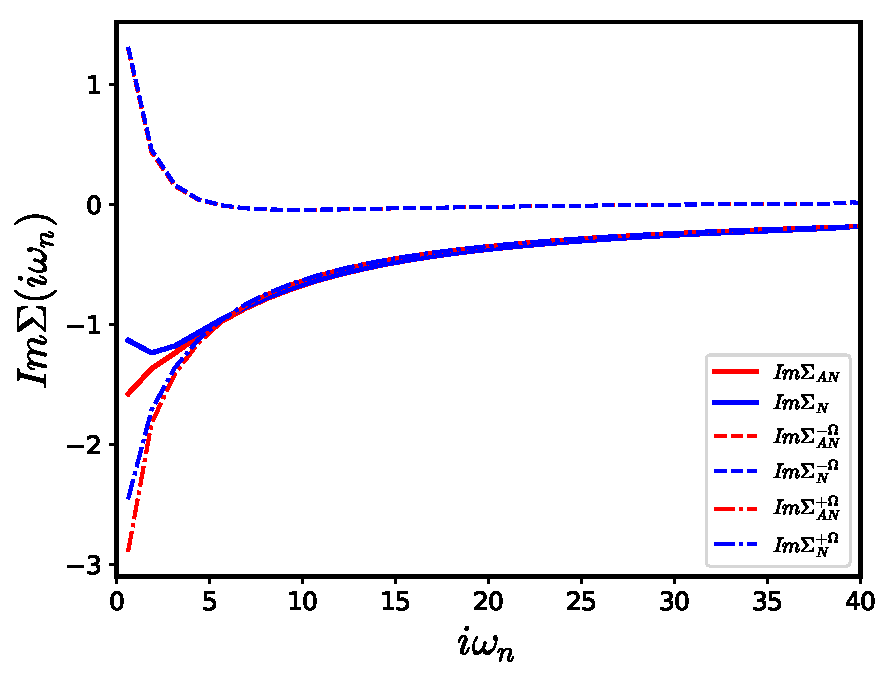
\includegraphics[width=0.9\linewidth]{fig3/self_energy.pdf}
    
\caption{ The imaginary part of the single particle self energy from Fig.~\ref{fig:Self_ Energy} deconstructed into its  $+\Omega$ and $-\Omega$ contributions at $U/t=5.6$, $\beta t =5$, $t^\prime /t=-0.3$, and $\mu=0$. \label{fig:sum_frequency}}
\end{figure}

Therefore, we first examine the behaviour of the self energy by decomposing it into positive and negative bosonic frequency contributions. The result is depicted in Fig. \ref{fig:sum_frequency}. The self-energy for this case is:

\begin{equation}
    Im\Sigma_k^{(\Omega,q)}= Im\Sigma_k^{(+ \Omega,q)}+Im\Sigma_k^{(- \Omega,q)}
\end{equation}

It can be seen that to have the accurate curve of self-energy for nodal and antinodal point we have to sum over positive and negative Bosonic frequencies. 


\noindent Then to see the contribution of zeroth Bosonic frequensy $(\Omega=0)$ we separate this frequency. The total self energy now is this summation:
\begin{equation}
    Im\Sigma_k(\omega)=Im\Sigma_k^{(\Omega,q)}= Im\Sigma_k^{(+ \Omega,q)}+Im\Sigma_k^{(- \Omega,q)} + Im\Sigma_k^{(\Omega=0,q)}
\end{equation}

 Results for each component are shown in Fig. \ref{fig:sum_frequency0}. We find that the largest contributions to the self energy come from $\Omega=0$ which are negative for all $i\omega_n>0$ and also show a negative contribution to $\Delta \Sigma$. The summations over positive and negative bosonic frequencies decay rapidly with fermionic frequency while the $\Omega=0$ contribution dominates the high frequency behavior.  We also observe that the positive bosonic contributions are primarily negative while the negative bosonic frequency contributions are primarily positive.  Interestingly, the summations over $\Omega>0$ and $\Omega<0$ show almost no momentum dependence.  All of the momentum dependence comes from $\Omega=0$ excitations which provide a slightly more negative contribution to $\Delta \Sigma_{AN}$ than for $\Delta \Sigma_N$. Further, the only positive contributions to $\Delta \Sigma$ come from the summation over $\Omega<0$.  Thus, deciding if $\Delta \Sigma$ is positive or negative rests on a subtle interplay between these three components. This is an element not mentioned in the original fluctuation diagnostics description  .\cite{Toschi}. These figures show that $\Delta \Sigma$ changes sign due to interplay of the $+\omega$ and $-\Omega$. 

\begin{figure}[ht]
\centering
    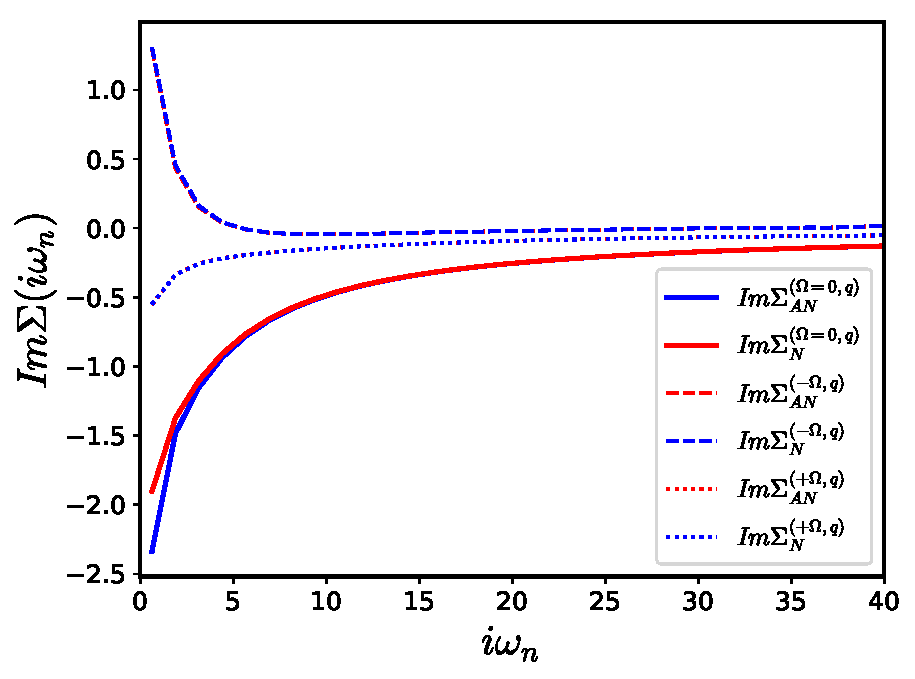
\includegraphics[width=0.9\linewidth]{fig3/self_energy_W0.pdf}
    
\caption{ The imaginary part of the single particle self energy from Fig.~\ref{fig:Self_ Energy} deconstructed into its  $+\Omega$ and $-\Omega$ contributions and the $\Omega=0$ contribution at $U/t=5.6$, $\beta t =5$, $t^\prime /t=-0.3$, and $\mu=0$. \label{fig:sum_frequency0}}
\end{figure}

Moreover, in Fig. \ref{fig:sum_n1} we show the contribution Bosonic frequencies in the self-energy of two first Fermionic frequencies. This figure reveals that the zeroth Bosonic frequency has the most contribution in the self-energy, so it's appropriate that we focus on these frequencies.

\begin{figure}[ht]
\centering
    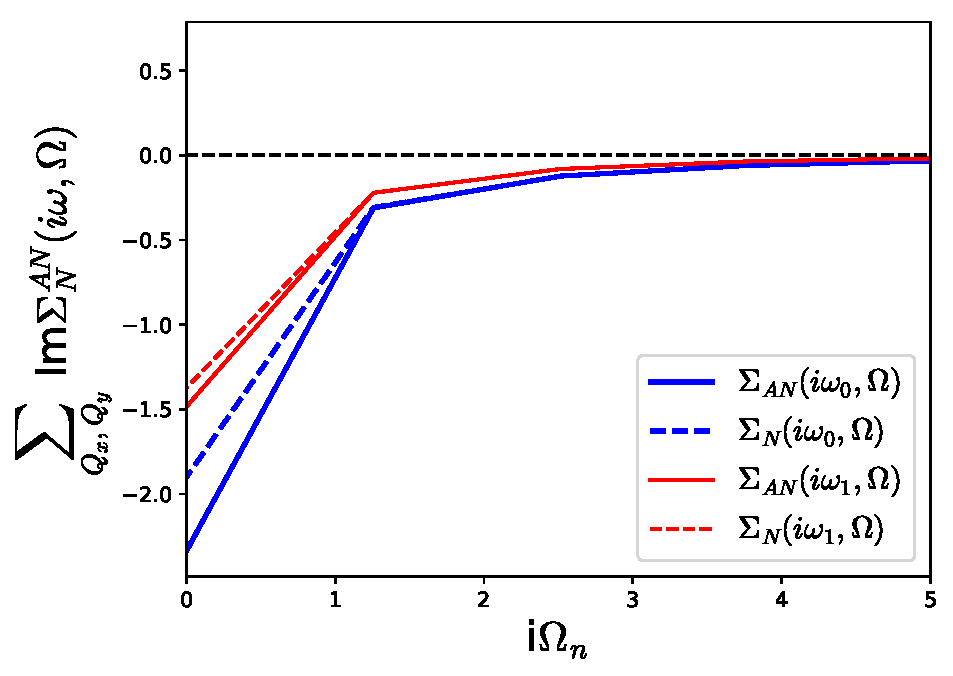
\includegraphics[width=0.9\linewidth]{fig3/summation_sigma_n1_n2.pdf}
    
\caption{ The imaginary part of the self energy deconstructed into its  $\omega_0$ and $\omega_1$ contributions at $U/t=5.6$, $\beta t =5$, $t^\prime /t=-0.3$, and $\mu=0$. The contribution of Bosonic frequencies has been shown. It can be seen that zeroth Bosonic frequency has the most contribution in the self energy. \label{fig:sum_n1}}
\end{figure}

\subsection{$\Delta\Sigma$}

In Fig. \ref{fig:deltasigma_all} we investigated the relation between density and $\Delta \Sigma$. Now we can study doping dependency in more details. We select a range of densities for which expect $\Delta \Sigma$ to switch sign. Results for $n=0.94, 1.0,$ and 1.1 are represented in Fig.~\ref{fig:delta_sigma} for $\Delta \Sigma^{(\Omega)}(q_x,q_y)$ which includes the total bosonic contributions at each $q_x$ and $q_y$ value.  
This allows us to notice particularly which $q$-vectors give FL ($\Delta \Sigma^{(\Omega)}>0$) contributions or nFL  ($\Delta \Sigma^{(\Omega)}<0$) contributions.  We concentrate on $U/t=5.6$ where nodal and antinodal differences happen. 

\begin{figure}[ht]
\centering
    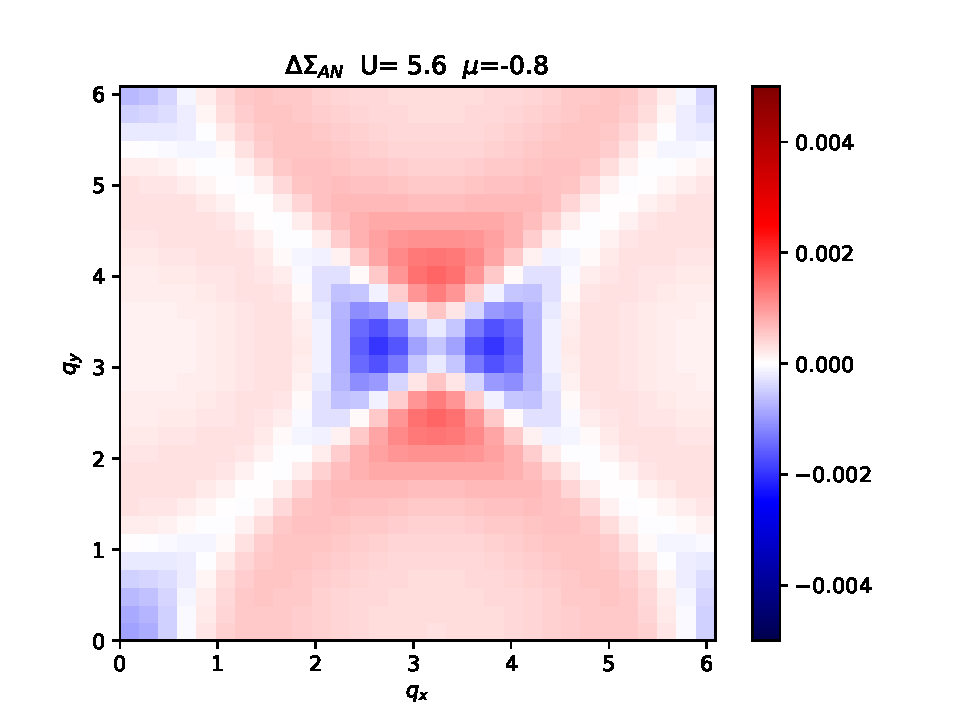
\includegraphics[width=0.45\linewidth]{fig3/c_5_-8_AN.pdf}
    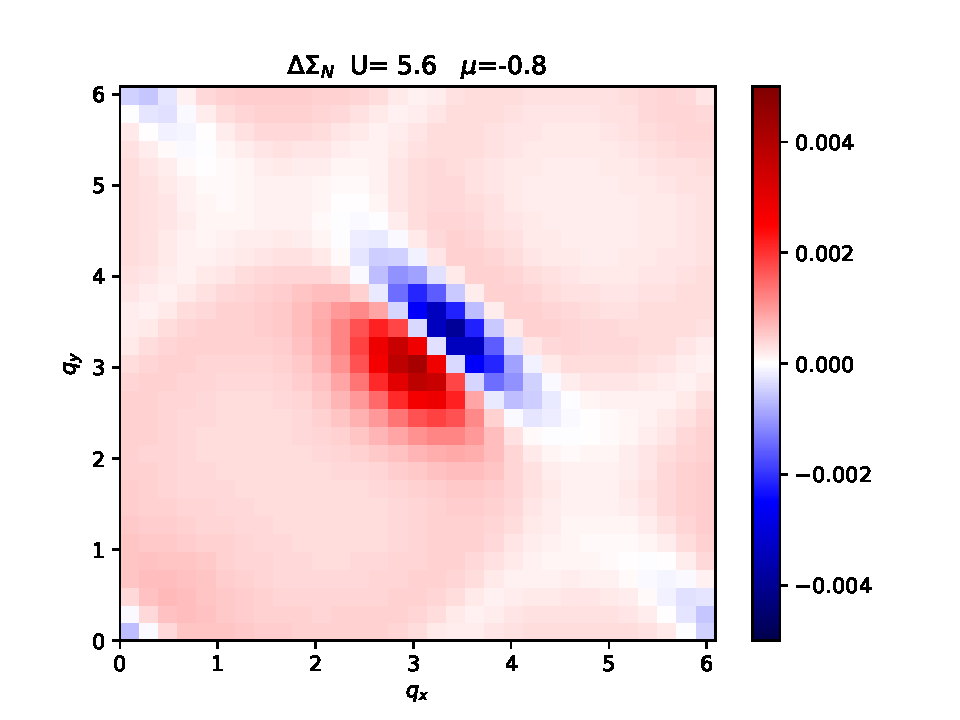
\includegraphics[width=0.45\linewidth]{fig3/c_5_-8_node.pdf}
    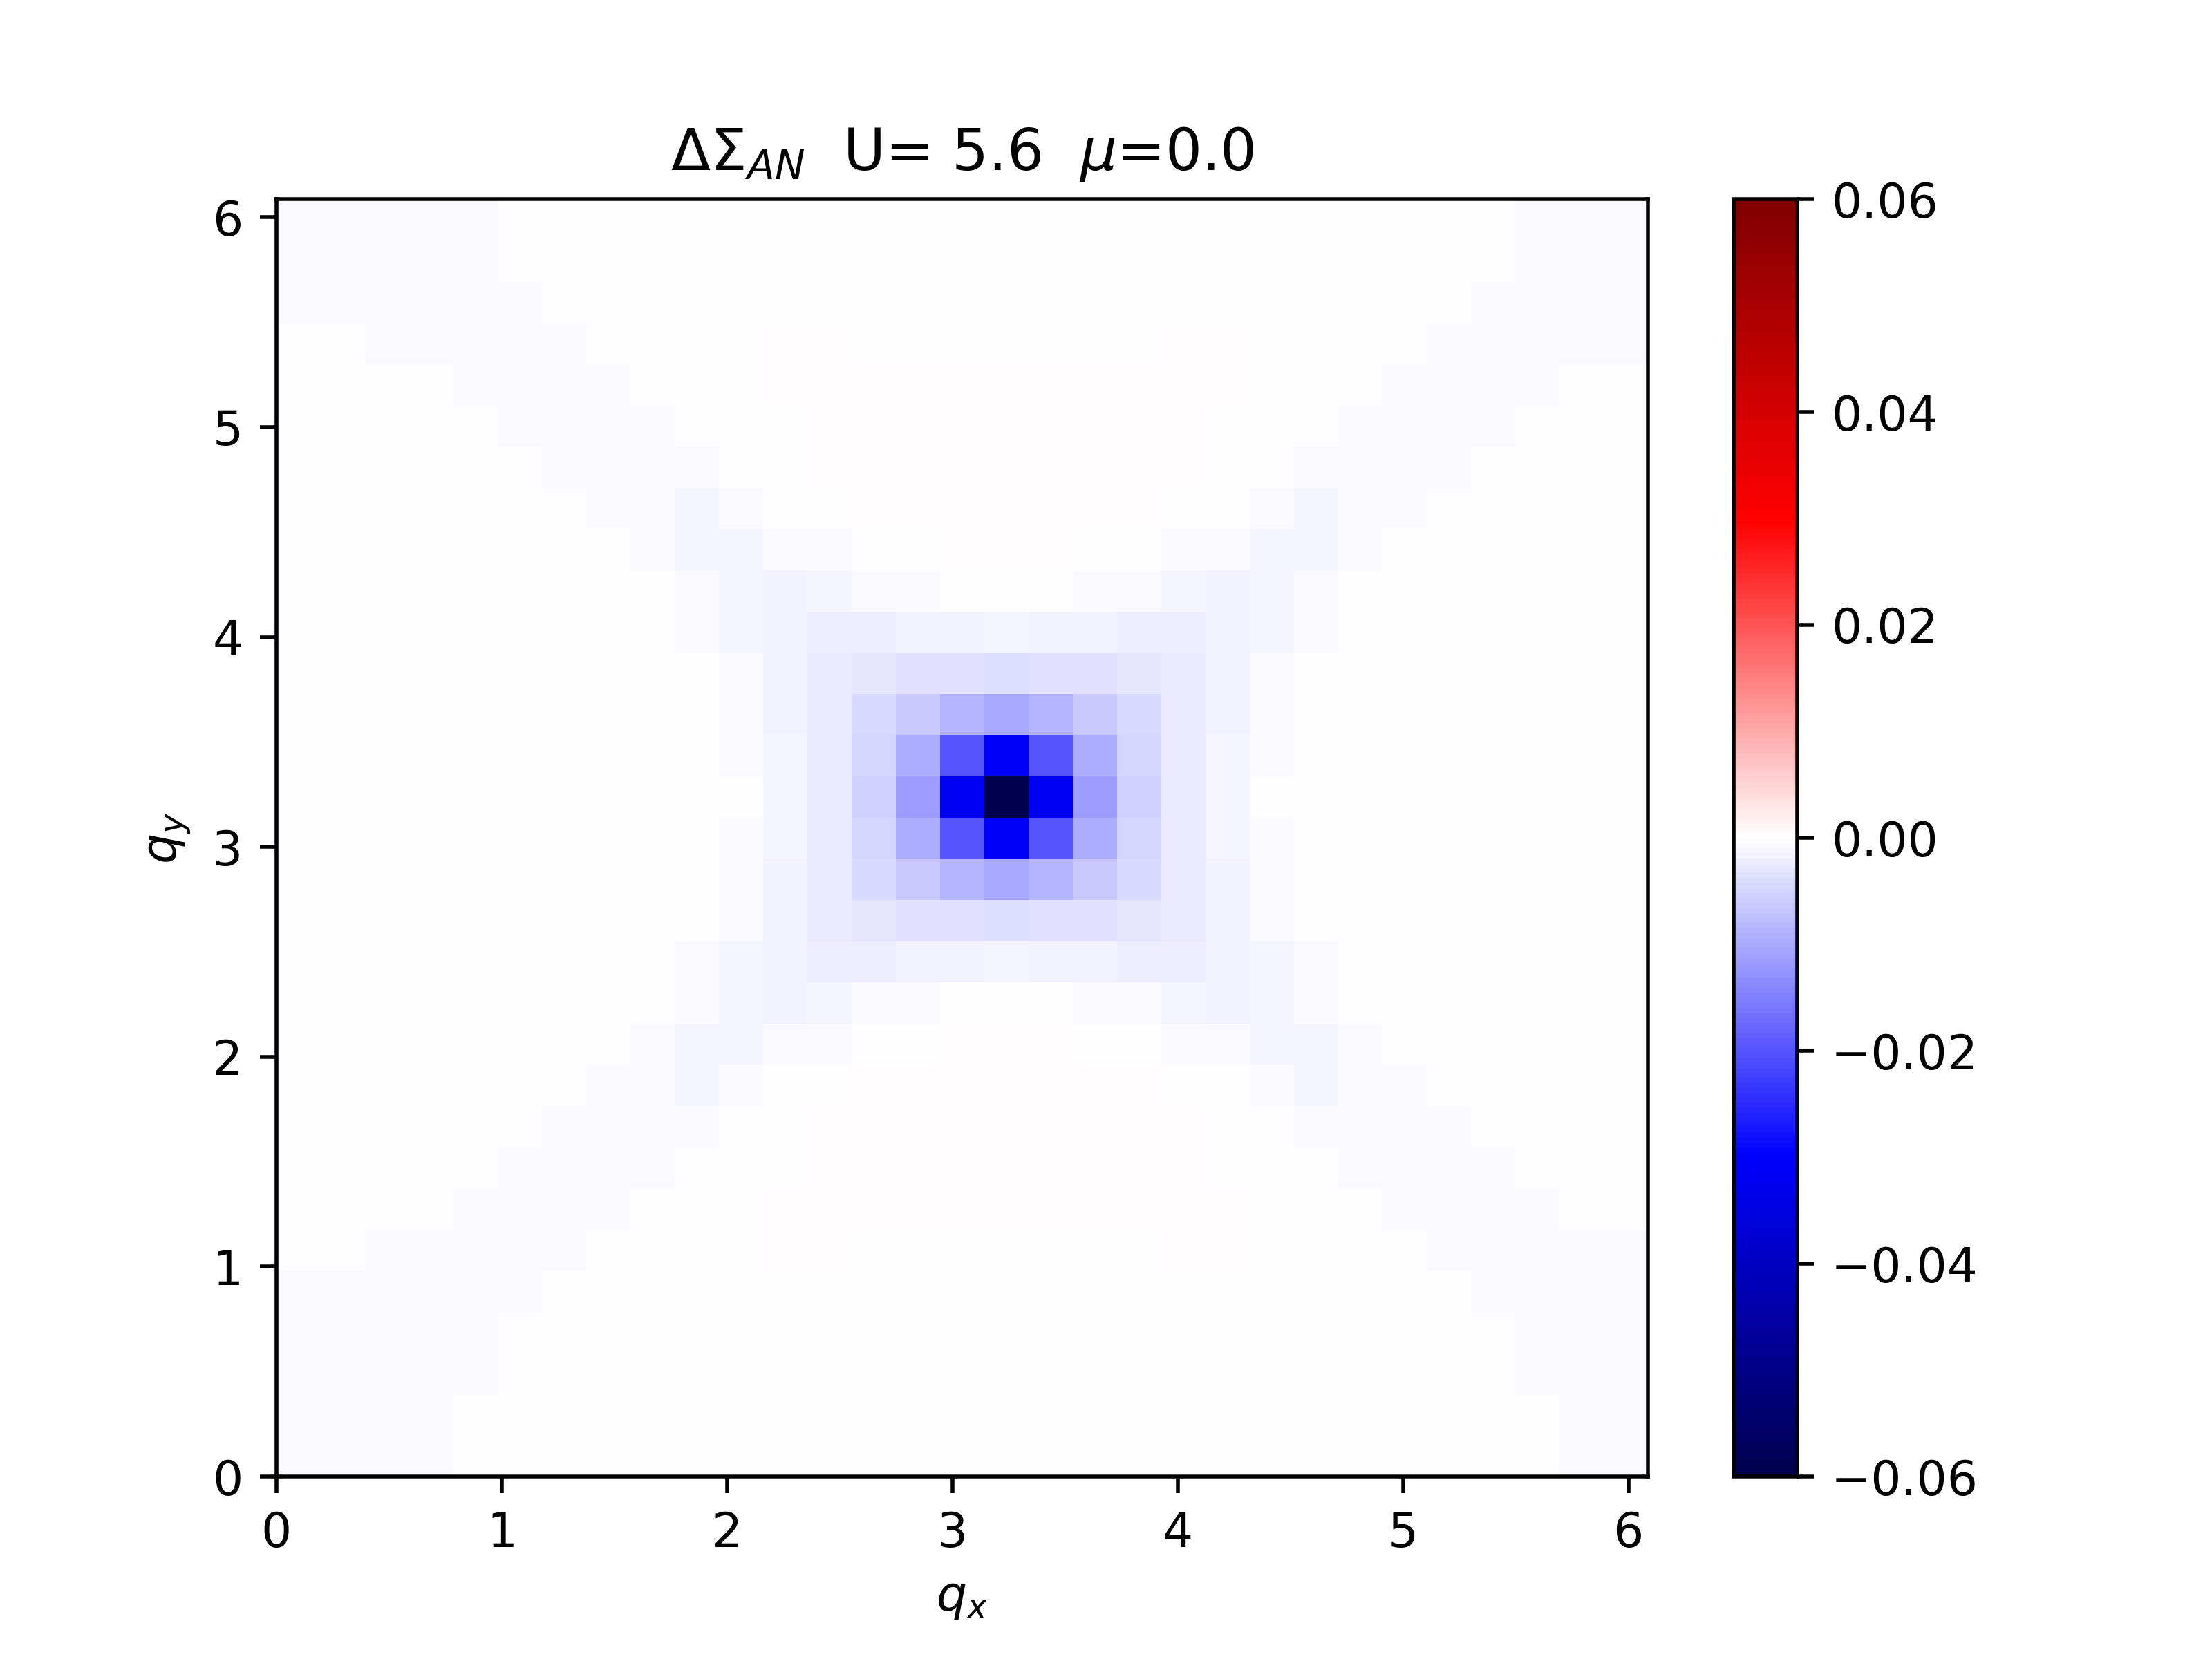
\includegraphics[width=0.45\linewidth]{fig3/c_5_0_AN.png}
    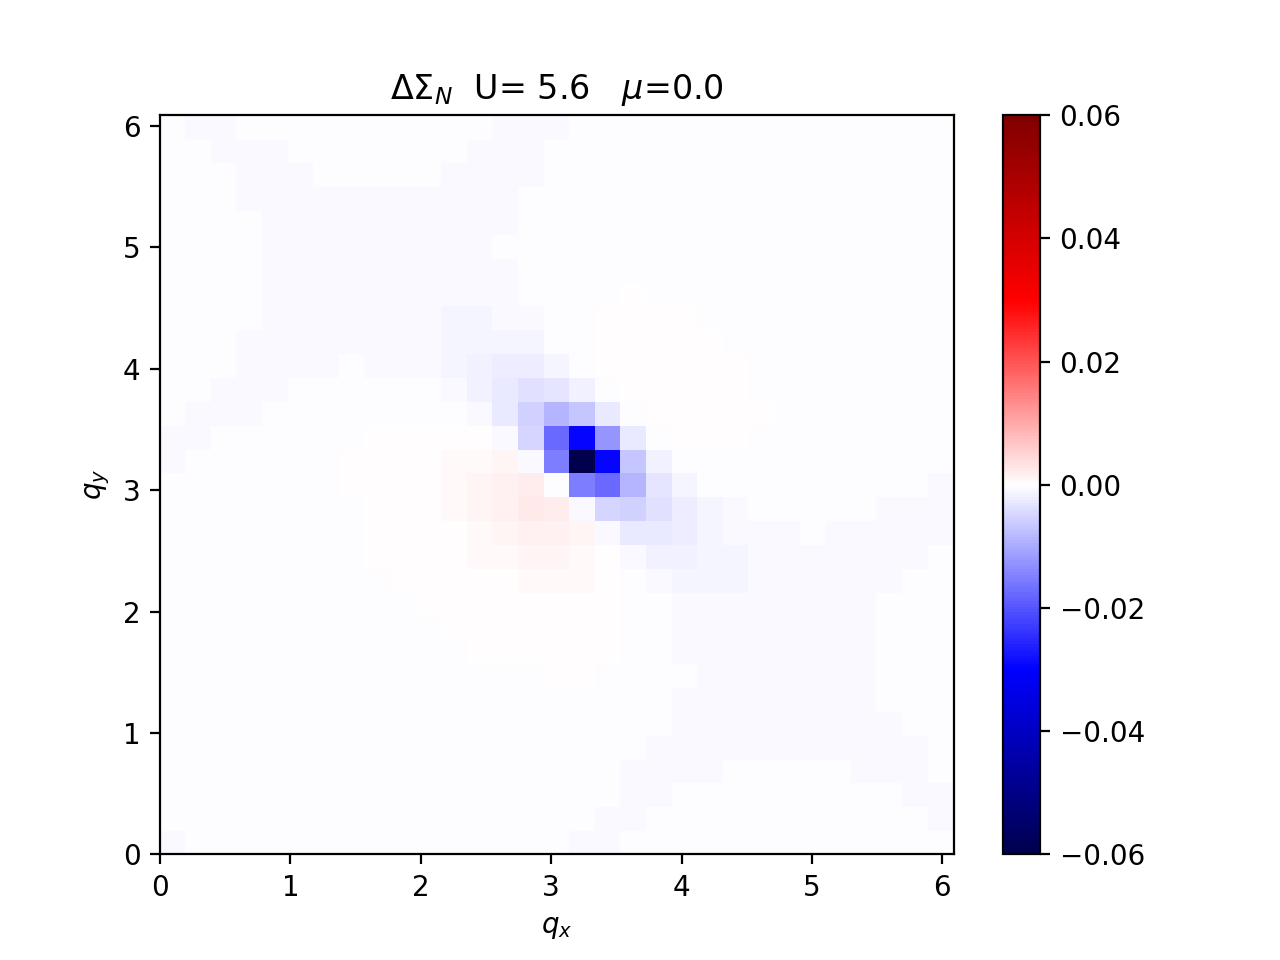
\includegraphics[width=0.45\linewidth]{fig3/c_5_0_node.png}
    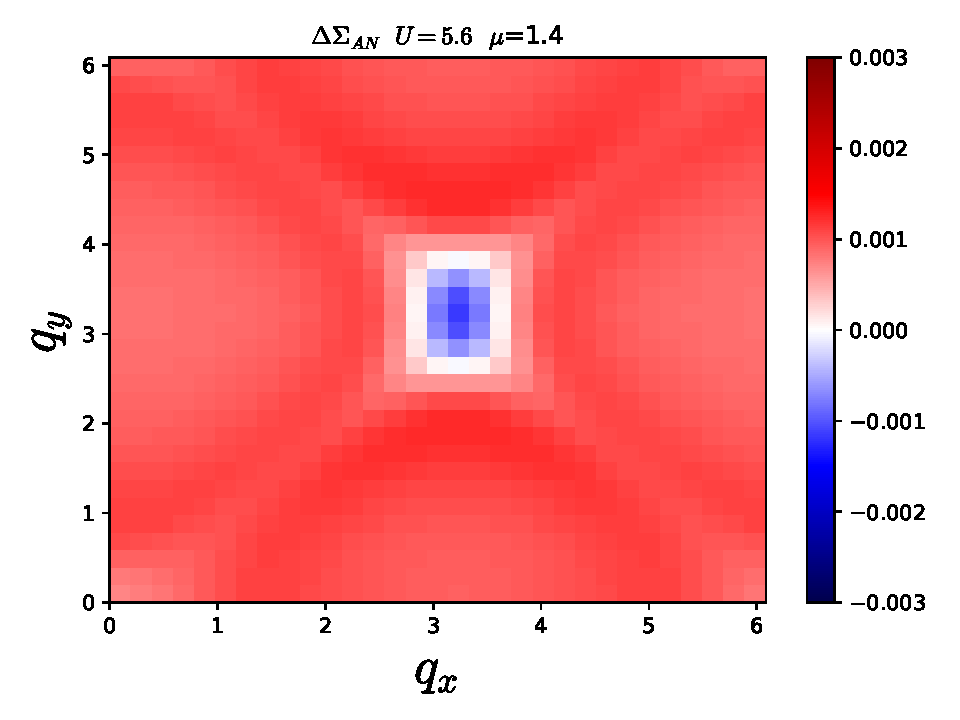
\includegraphics[width=0.45\linewidth]{fig3/c_5_14_AN.pdf}
    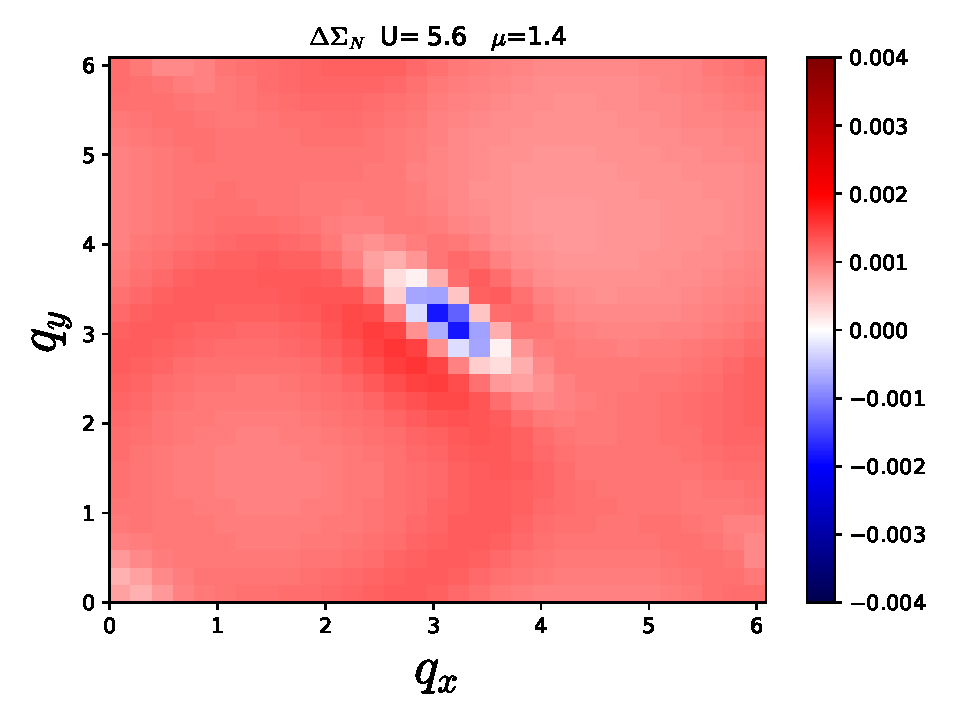
\includegraphics[width=0.45\linewidth]{fig3/c_5_14_node.pdf}
    
\caption{ Color Plots: $\Delta \Sigma^{(\Omega)}(q_x,q_y)$ for nodal and anti- nodal momenta at $U/t= 5.6$ for $n=0.94$ (top row), 1 (middle) and 1.1 (bottom row) corresponding to chemical potentials of $\mu/t = -0.8, 0, 1.4 $ respectively.  
\label{fig:delta_sigma}}
\end{figure}


 We see that both the antinodal and nodal frames in the top row of Fig.~\ref{fig:delta_sigma} (left and right columns respectively). These figures show complicated structure which include both positive and negative contributions.
From Fig.~\ref{fig:deltasigma_all} we know that the total antinodal $\Delta \Sigma_{AN}<0$ while the total nodal $\Delta \Sigma_{N} >0$ when these results are summed over $q_x$ and $q_y$. 
For the anti-nodal frame most $q$-vectors provide positive contributions, which are very weak, with strong positive contributions above and below $(\pi,\pi)$. Also we can see there are strong negative contributions to the left and right of $(\pi,\pi)$.
In the nodal case again most of the $q$-vectors give weak positive contribution and we can see both strong negative and positive peaks. In this case the strong positive feature near $(\pi,\pi)$ overcomes the strong negative feature which finally gives an overall $\Delta \Sigma_N >0$.

 At half filling case all $q$-vectors give negative contributions, with the strongest feature near $q=(\pi,\pi)$. 
While, at $n=1.1$ most of the $q$-vectors provide strong positive contributions, but the $(\pi,\pi)$ feature remains strong and negative resulting in both the nodal and antinodal columns having a total $\Delta\Sigma>0$ as we know is the case from Fig.~\ref{fig:deltasigma_all}.

Finally, from the original fluctuation diagnostics work\cite{Toschi} we understand that the observation of the broad background for $n=1.1$ might suggest that the spin channel is not the best (most compact) basis for describing the electron doped system.


\begin{figure}[ht]
\centering
    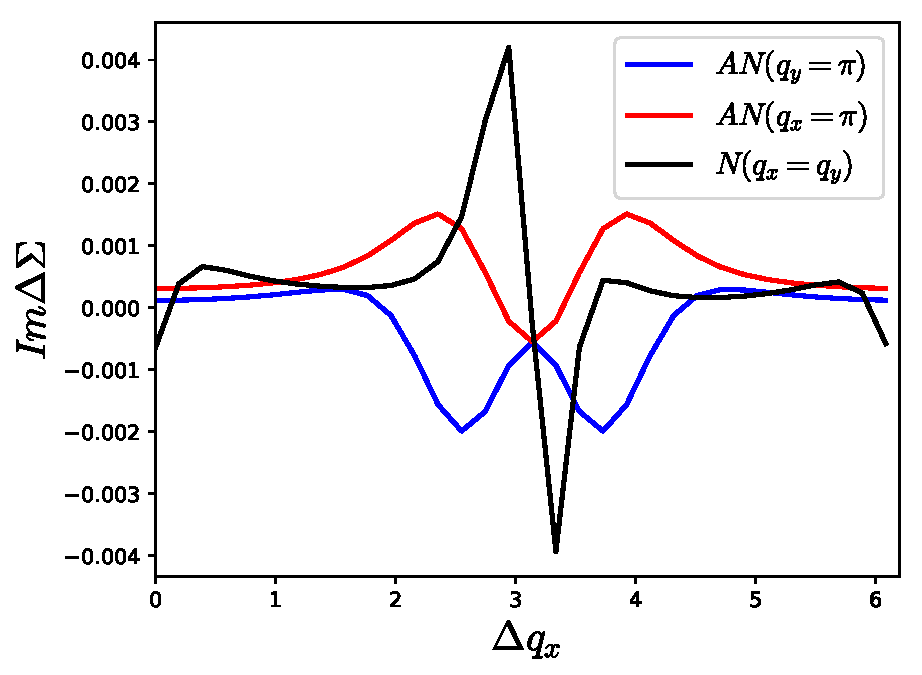
\includegraphics[width=0.45\linewidth]{fig3/3cuts_mu-8.pdf}
    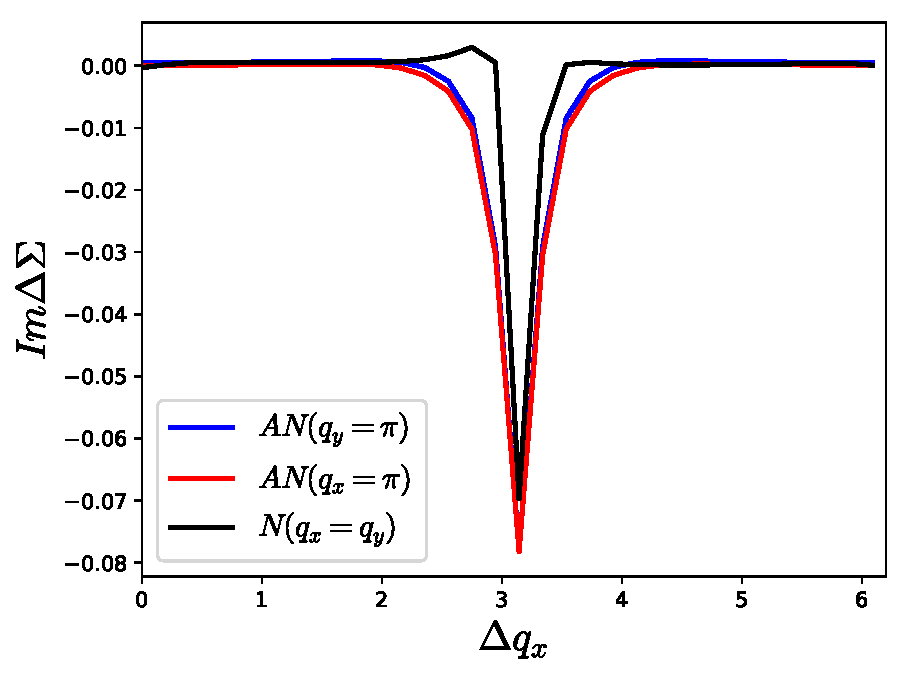
\includegraphics[width=0.45\linewidth]{fig3/3cuts_mu0.pdf}
    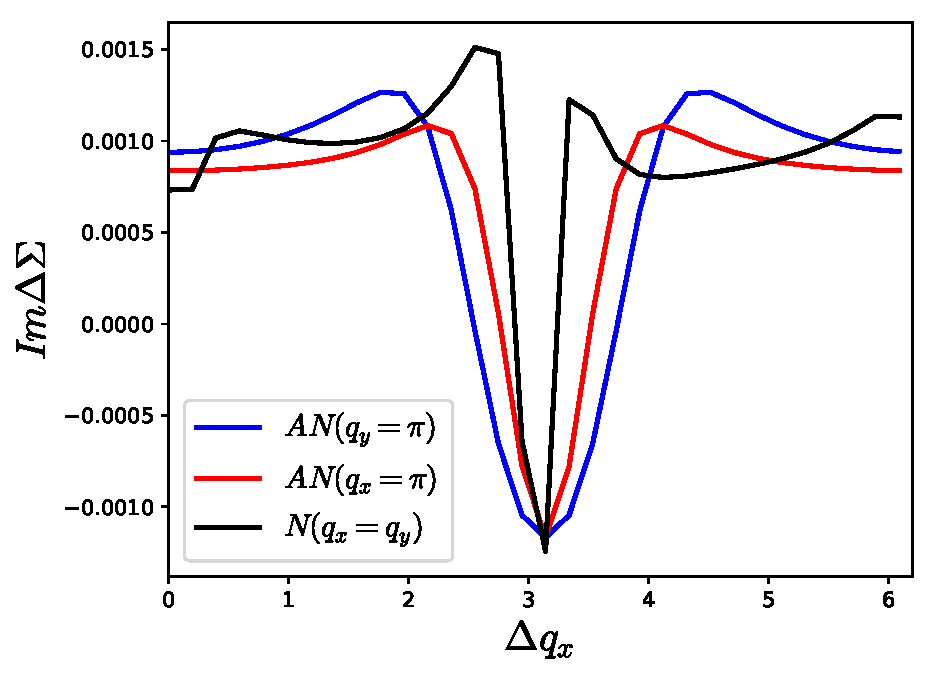
\includegraphics[width=0.45\linewidth]{fig3/3cuts_mu14.pdf}
    
\caption{This figure shows cuts of $\Delta \Sigma^{(\Omega)}(q_x,q_y)$ for: (blue) a cut in the antinodal result along the path from $(0,\pi) \to (2\pi,\pi)$, (red) a cut in the antinodal result along the path from $(\pi,0) \to (\pi,2\pi)$, and (black) a cut in the nodal result along the path from $(0,0)\to(2\pi,2\pi)$. Each path is plotted by its length in the x-axis, normalized by the total length of the cut. The top left plot is provided for $U=5.6$ and $\mu=-0.8$, top right plot $U=5.6$ and $\mu=0.0$, and the bottom plot $U=5.6$ and $\mu=1.4$.
\label{fig:3cuts}}
\end{figure}

To  analyze the color plots of Fig. \ref{fig:deltasigma_all}, plots of Fig.~\ref{fig:3cuts} includes high symmetry cuts through the Brillouin zone, which provide horizontal, vertical, and diagonal cuts through the datasets in Fig.~\ref{fig:deltasigma_all}. This plots shows cuts of $\Delta \Sigma^{(\Omega)}(q_x,q_y)$ for: (blue) for the antinodal result along the path from $(0,\pi) \to (2\pi,\pi)$, (red) is a cut for the antinodal result along the path from $(\pi,0) \to (\pi,2\pi)$, and (black) for the nodal result along the path from $(0,0)\to(2\pi,2\pi)$. The top left plot is provided for $U=5.6$ and $\mu=-0.8$, top right plot $U=5.6$ and $\mu=0.0$, and the bottom plot $U=5.6$ and $\mu=1.4$.

In Fig.\ref{fig:delta_sigma} for $\mu=0.8$ we see a complicated structure with two negative pikes left and right side of $(\pi,\pi)$ point and two positive points below and above $(\pi,\pi)$ point. In top-left plot of Fig.\ref{fig:3cuts} we showed exactly that for Anti-Nodal points there are two negative pikes by using a horizontal cut through the BZ $(q_y=\pi)$, and vertical cut $(q_x=\pi)$ reveal that there are two positive pikes above and below of $(\pi,\pi)$. For Nodal case, a diagonal cut $(q_x=q_y)$ shows a positive pike before $(\pi,\pi)$ and a negative pike after $(\pi,\pi)$.

For the half-filling case In Fig.\ref{fig:delta_sigma}  in both Nodal and Anti-Nodal, $\Delta \Sigma=0$ and there is a strong negative pike at the $(\pi,\pi)$, which we can see the same result in top right plot of Fig.\ref{fig:3cuts}. Finally, for $\mu=1.4$ in Fig. \ref{fig:delta_sigma} we saw that almost $\Delta \Sigma$ for both Nodal and Anti-Nodal is positive except at $(\pi,\pi)$ , which the bottom plot of Fig. \ref{fig:3cuts} depicts the same result.



